% %%%%%%%%%%%%%%%%%%%%%%%%%%%%%%%%%%%%%%%%%%%%%%%%%%%%%%%%%%%%%%%%%%%%%%%%%%%%%%%%%
%
%	MODELO LaTeX PARA ELABORACAO DE TESES E DISSERTACOES DO PPGEC/UFRGS 
%  --------------------------------------------------------------------
%	Versão:	v2.2 (03/03/2021) - informações em README.md
%
%
%	Creditos
%   --------
%
%		Autores:	Augusto Bopsin Borges (augusto.borges@ufrgs.br)
%					Rodrigo Escolante Pereira (rodrigoescolante@gmail.com)
%					Felipe Pinto da Motta Quevedo (00152604@ufrgs.br)
%
%
% %%%%%%%%%%%%%%%%%%%%%%%%%%%%%%%%%%%%%%%%%%%%%%%%%%%%%%%%%%%%%%%%%%%%%%%%%%%%%%%%%
%
%	Instruções para incluir a ficha catalográfica
%  ----------------------------------------------
%
%	Após defendido o trabalho se insere a ficha catalográfica. Para inserção
%	siga os seguintes passos:
%
%	1) acesse: https://sabi.ufrgs.br/servicos/publicoBC/ficha.php
%	2) preencha seus dados no site
%	3) gere o arquivo pdf
%	4) nomeioe-o como "ficha"
%	5) e copie-o para a pasta /pre/
%	6) deixe descomentado o comando \imprimirficha nos elementos pré-textuais
%
%
% %%%%%%%%%%%%%%%%%%%%%%%%%%%%%%%%%%%%%%%%%%%%%%%%%%%%%%%%%%%%%%%%%%%%%%%%%%%%%%%%%
%
%	Opções da classe ppgec.cls
%  ----------------------------
%
%		Essa classe utiliza como base a classe abnTex2.cls v-1.9.7 laurocesar
% 		Copyright 2012-2018 by abnTeX2 group at https://www.abntex.net.br/ 
%		
%		Por padrao a classe ppgec.cls esta configurada para tese, dissertações e
% 		qualificações com folha A4, tamanho de fonte 12pt e configuracao de impressao
%		em apenas um lado da folha. Ao usuário, porém, estao disponiveis algumas 
%		opções de configuração:
%
%		TIPO DE DOCUMENTO
%			doutorado 	: opção para tese de doutorado
%			mestrado 	: opção para dissertação de mestrado
%			qdoutorado 	: opção para qualificação de doutorado
%			qmestrado 	: opção para qualificação de mestrado
%
%		AREA DE CONCENTRAÇÃO
%			estrutura 	: opção para área de concentração em estrutura
%			geotecnia 	: opção para área de concentração em geotecnia
%
%		LINGUA
%			pt			: português
%			en			: inglês
%			sp			: espanhol
%
%
\documentclass[doutorado,estrutura,pt]{ppgec}
%	
% %%%%%%%%%%%%%%%%%%%%%%%%%%%%%%%%%%%%%%%%%%%%%%%%%%%%%%%%%%%%%%%%%%%%%%%%%%%%%%%%%
%
\usepackage{multirow}


% Preencha o arquivo dados.tex com os teus dados
% %%%%%%%%%%%%%%%%%%%%%%%%%%%%%%%%%%%%%%%%%%%%%%%%%%%%%%%%%%%%%%%%%%%%%%%%%%%%%%%%%
%
%	DADOS.tex 
%  -----------
%
%	Neste arquivo você escreve os dados necessários do seu trabalho.
%
% %%%%%%%%%%%%%%%%%%%%%%%%%%%%%%%%%%%%%%%%%%%%%%%%%%%%%%%%%%%%%%%%%%%%%%%%%%%%%%%%%
%
%
% Titulo, local, data e data completa
\titulo{Análise Computacional das Deformações em Túneis Profundos considerando o Acoplamento Plasticidade-Viscoplasticidade}
\local{Porto Alegre}
\data{2021}
\qualdatacompleta{10 de dezembro de 2021} % ou [Mounth] [day^{th}] 202X}
%
% Palavras-chave
\quaispalavraschave{túneis profundos, elastoplasticidade, viscoplasticidade, método dos elementos finitos, leis constitutivas}
\quaiskeywords{deep tunnels. elastoplasticity. viscoplasticity. finite element method. constitutive laws}
\quaispalabrasclave{túneles profundos, elastoplasticidad, viscoplasticidad, método de elementos finitos, leyes consitutivas}
%
% Dados do autor
\autor{Felipe Pinto da Motta Quevedo}
\qualcitarautor{Quevedo, F. P. M.}
\qualemailautor{motta.quevedo@ufrgs.br}
%
% Dados do orientador
\orientador{Prof. Samir Maghous}
\qualtitorientador{Dr. pela École Nationale des Ponts et Chaussées}
\qualgeneroorientador{M}
%
% Dados coorientador
\temcoorientador{Sim}
\coorientador{Profa. Denise Bernaud Maghous}
\qualtitcoorientador{Dra. pela École Nationale des Ponts et Chaussées}
\qualgenerocoorientador{F}
%
% Dados do coordenador do curso
\qualcoordenador{Nilo Consoli}
\qualtitcoordenador{Ph.D. pela Concordia University, Canadá}
\qualgenerocoordenador{M}
%
% Dados sobre a banca (no máximo 6)
\quantosmembrosbanca{3}
%
% Adicionando membros da banca e dados deles
\addtext{Prof. Américo Campos Filho}								% Nome da banca
\addtext{UFRGS}														% Instituição da banca
\addtext{Dr. pela Escola Politécnica da Universidade de São Paulo}	% Titulação da banca
%
\addtext{Prof. Mauro de Vasconcellos Real}
\addtext{FURG}
\addtext{Dr. pela Universidade Federal do Rio Grande do Sul}
%
\addtext{Prof. Liércio André Isoldi}
\addtext{FURG}
\addtext{Dr. pela Universidade Federal do Rio Grande do Sul}
%
%
% Carregando pacotes e macros adicionais definidas pelo usuário
% %%%%%%%%%%%%%%%%%%%%%%%%%%%%%%%%%%%%%%%%%%%%%%%%%%%%%%%%%%%%%%%%%%%%%%%%%%%%%%%%%
%
%	PACOTES_MACROS.tex 
%  --------------------
%
%	Este arquivo é lido no preâmbulo do main.tex e portanto, você pode inserir nele:
%
%		- pacotes que não estão na classe ppgec.cls (veja se a classe já não possui)
%		- suas próprias macros
%		- qualquer outro comando de preâmbulo
%
% %%%%%%%%%%%%%%%%%%%%%%%%%%%%%%%%%%%%%%%%%%%%%%%%%%%%%%%%%%%%%%%%%%%%%%%%%%%%%%%%%
%
%	Pacotes
%	-------
%
\usepackage{float}	% permite posicionar a figura entre parágrafos usando H
%
%
% %%%%%%%%%%%%%%%%%%%%%%%%%%%%%%%%%%%%%%%%%%%%%%%%%%%%%%%%%%%%%%%%%%%%%%%%%%%%%%%%%
%
%	Macros e configurações de pacotes
%	---------------------------------
%
% Imprimir anexo pdf: \imprimiranexopdf{nome do arquivo}{título do anexo}{primeirapagina}{proximaspaginas}
\newcommand{\imprimiranexopdf}[4]{
	\includepdf[pages=#3,pagecommand=\chapter{#2},scale=0.92,offset=0 -95]{#1}
	\includepdf[pages=#4,pagecommand={}]{#1}
}
%
%
% %%%%%%%%%%%%%%%%%%%%%%%%%%%%%%%%%%%%%%%%%%%%%%%%%%%%%%%%%%%%%%%%%%%%%%%%%%%%%%%%%
%
%	Outros comandos de preâmbulo
%	----------------------------
\newcommand{\gammal}{\underline \gamma}
\newcommand{\fl}{\underline f}
\newcommand{\Tl}{\underline T}
\newcommand{\euml}{\underline{e}_1}
\newcommand{\edoisl}{\underline{e}_2}
\newcommand{\etresl}{\underline{e}_3}
\newcommand{\xl}{\underline x}
\newcommand{\sigmall}{\underline{\underline \sigma}}
\newcommand{\nl}{\underline n}
\newcommand{\divl}{\underline \nabla \cdot}
\newcommand{\ul}{\underline u}
\newcommand{\Fll}{\underline{\underline F}}
\newcommand{\Umll}{\underline{\underline 1}}
\newcommand{\greenll}{\underline{\underline e}}
\newcommand{\varepsilonll}{\underline{\underline \varepsilon}}
\newcommand{\Dllll}{\underline{\underline{\underline{\underline D}}}}
\newcommand{\Umllll}{\underline{\underline{\underline{\underline 1}}}}
\newcommand{\alphal}{\underline \alpha}
\newcommand{\ql}{\underline q}
\newcommand{\sll}{\underline{\underline s}}
\newcommand{\dgdsll}{\underline{\underline {g_{_\sigma}}}}
\newcommand{\gllum}{\underline{\underline {g_{_1}}}}
\newcommand{\glldois}{\underline{\underline {g_{_2}}}}
\newcommand{\glltres}{\underline{\underline {g_{_3}}}}
\newcommand{\hl}{\underline h}
\newcommand{\dfdsll}{\underline{\underline {f_{_\sigma}}}}
\newcommand{\dfdql}{\underline{f_{_q}}}
\newcommand{\dul}{\underline {\delta u}}
\newcommand{\dvarepsilonll}{\underline{\underline {\delta \varepsilon}}}

\newcommand{\varepsilonl}{\underline{\varepsilon}}
\newcommand{\Dll}{\underline{\underline D}}
\newcommand{\sigmal}{\underline \sigma}
\newcommand{\dgdsl}{\underline{g_{_\sigma}}}
\newcommand{\Uml}{\underline{1}}
\newcommand{\dvarepsilonl}{\underline{\delta \varepsilon}}
\newcommand{\Nll}{\underline{\underline N}}
\newcommand{\Bll}{\underline{\underline B}}
\newcommand{\Fl}{\underline{F}}
\newcommand{\Kll}{\underline{\underline K}}
%
%
%	
% %%%%%%%%%%%%%%%%%%%%%%%%%%%%%%%%%%%%%%%%%%%%%%%%%%%%%%%%%%%%%%%%%%%%%%%%%%%%%%%%%
%
%
% Iniciando o ambiente do documento
\begin{document}
%
% Elementos pré-textuais
\imprimircapa				% obrigatório
\imprimirfolhaderosto		% obrigatório
%\imprimirficha				% obrigatório
%\imprimirerrata			% opcional
\imprimirfolhadeaprovacao	% obrigatório
\imprimirdedicatoria		% opcional
\imprimiragradecimentos		% opcional
\imprimirepigrafe			% opcional
\imprimirresumo				% obrigatório
\imprimirabstract			% obrigatório
\imprimirlistafiguras		% opcional
\imprimirlistaquadros		% opcional
\imprimirlistatabelas		% opcional
\imprimirlistasiglas		% opcional
\imprimirlistasimbolos		% opcional
\imprimirsumario			% obrigatório
%
% Carrega configuração dos elementos textuais
\textualconfig
%
% Elementos textuais: capitulos
\chapter{Introdução}\label{introducao}

Os túneis são grandes obras de engenharia que, além de causar grande admiração, atendem a diversas finalidades, sendo a mais conhecida aquela de transpor barreiras geológicas como, por exemplo, montanhas e canais marítimos, trazendo maior eficiência no transporte de recursos e pessoas. Também devido à crescente preocupação com o meio ambiente e com a preservação da superfície, essas estruturas têm sido cada vez mais empregadas em grandes cidades, melhorando assim a mobilidade urbana como, por exemplo, em metrôs e servindo de suporte para serviços públicos, tais como redes de água, esgoto, gás e eletricidade. São também empregados em hidroelétricas, laboratórios subterrâneos, instalações profundas para armazenamento de material radioativo e mineração.

Há, no entanto, um risco intrínseco associado a essas grandes obras, uma vez que o subsolo é em grande parte desconhecido e possui um comportamento complexo. Apesar de muitas dessas construções serem finalizadas com sucesso, ocorrem incidentes que levam a atrasos, custos excessivos e, em alguns casos, consequências mais significativas, tais como, danos em patrimônios de terceiros e perdas de vidas. Esses imprevistos estão relacionados a uma série de fatores que vão desde incertezas geológicas, cálculos inadequados, processo construtivo inapropriado e insuficiente monitoramento das deformações \textit{in loco}. Não obstante, uma parte destes acidentes está relacionada com a dificuldade em prever e modelar o comportamento mecânico dessas grandes obras.

Um dos comportamentos de difícil modelagem e ainda estudado é justamente a interação entre o comportamento instantâneo e o diferido dessas estruturas. Este comportamento pode ter um impacto significativo nas deformações e estabilidade da cavidade. A plastificação no entorno do maciço, o fechamento gradual da seção do túnel, a extrusão da face de escavação e a sobrecarga sobre o revestimento, podem se desenvolver durante o tempo construtivo, no curto prazo, ou ainda, meses e anos após a construção do túnel no médio e longo prazo. Esse comportamento pode causar deformações excessivas (\autoref{redução_base_turin}), danos ao revestimento (\autoref{ruptura_china}) e, em alguns casos, pela magnitude dos efeitos, acarretar o colapso da região no entorno do túnel.

\begin{figure}[H]
	\begin{center}
		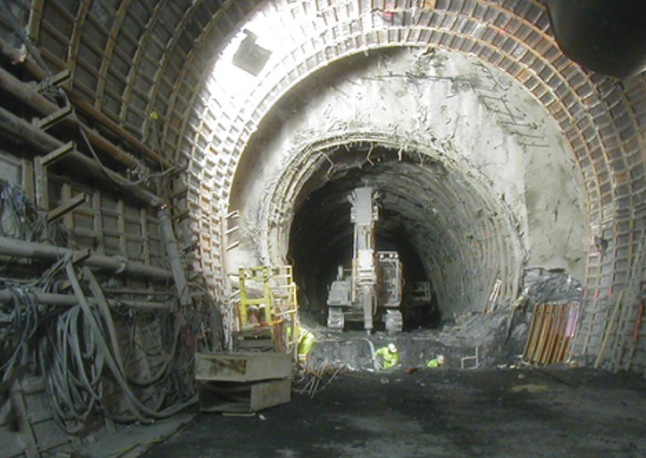
\includegraphics[width=12cm, height=8.33cm]{0101-redução da seção transversal do túnel de Base Lyon-Turin.png}
	\end{center}
	\caption{\label{redução_base_turin}Redução da seção transversal do Túnel de Base Lyon Turin na fronteira entre frança e Itália (fonte: \citeonline[p. 41]{Barla2010})}
\end{figure}

\begin{figure}[H]
	\begin{center}
		\includegraphics[width=12cm, height=8.33cm]{0102-ruptura do suporte em uma mina de carvão na china.png}
	\end{center}
	\caption{\label{ruptura_china}Ruptura do suporte (perfil de aço) em uma mina de carvão na China (fonte: \citeonline[p. 192]{Manchao2015})}
\end{figure}
 
Além da estabilidade da cavidade, a escolha da tecnologia para a escavação é altamente influenciada pela magnitude dessa condição diferida no tempo. Por exemplo, em escavações com tuneladoras (TBM - \textit{Tunnel Boring Machines}), as pressões que se desenvolvem sobre a blindagem podem causar uma série de dificuldades como o aprisionamento da máquina (tal como visto em Ramoni e Anagnostou (\citeyear{Ramoni2010a,Ramoni2010b}). É sabido também que suportes flexíveis ou que apresentam um comportamento diferido no tempo (perfis metálicos deslizantes ou concreto projetado) são mais adequados do que suportes rígidos, uma vez que permitem um certo grau de acomodação dessas deformações diferidas.

Muitos estudos consideram leis constitutivas empírico-experimentais, viscoelásticas ou ainda viscoplásticas em suas análises diferidas no tempo, contudo, todos esses modelos partem de um comportamento instantâneo elástico o que pode não corresponder com a realidade, uma vez que o maciço pode possuir um comportamento instantâneo elastoplástico.

Em vista da importância do tema para a comunidade geotécnica de túneis, a presente tese faz o desenvolvimento de uma relação constitutiva para lidar com o comportamento diferido no tempo, considerando um modelo viscoplástico, conjuntamente com o comportamento instantâneo dado por um modelo elastoplástico. 

Além dessa introdução, esse trabalho está dividido em mais 7 capítulos.

O \textbf{capítulo 2} tem a finalidade de esclarecer o mais objetivamente possível o que se pretende desenvolver nessa tese, explicitando o tema, os objetivos a alcançar, as delimitações  adotadas e o delineamento de como se deu o trabalho.

O \textbf{capítulo 3} foi introduzido com o intuito de apresentar brevemente alguns aspectos do estado da arte de túneis. Portanto, esse capítulo resume brevemente os métodos de escavação, os elementos e técnicas de pré-suporte, os revestimentos e principais aspectos considerados em estudos numéricos recentes. Portanto, esse capítulo é opcional aos leitores mais experientes e pode ser ignorado sem prejuízo ao entendimento do trabalho restante.

O \textbf{capítulo 4} tem por finalidade instruir o leitor no comportamento mecânico de túneis e seus conceitos fundamentais. Esse capítulo está dividido de acordo com os principais fatores que influenciam o campo de tensões e deformações no entorno dessas estruturas, tais como, o processo de escavação, o comportamento reológico do maciço, a forma da seção, a profundidade do túnel, a proximidade da superfície e a interação com o revestimento. Nesse capítulo é dada uma maior ênfase na reologia do maciço, caracterizando o comportamento instantâneo e diferido, que são justamente os comportamentos almejados no modelo proposto dessa tese. Ao final, também são apresentados alguns estudos que consideraram leis elastoplástica-viscoplástica no comportamento do maciço.

O \textbf{capítulo 5} descreve o modelo teórico implementado esclarecendo as principais hipóteses e explicando cada uma das leis constitutivas adotadas (elástica, elastoplástica e viscoplástica) de forma genérica. No final desse capítulo é descrito então o modelo constitutivo acoplado elastoplástico-viscoplástico desenvolvido nessa tese.

O \textbf{capítulo 6} se refere à solução numérica do modelo teórico implementado. Portanto, descreve a discretização espacial em elementos finitos, incluindo os tipos de elementos que são utilizados, o método de solução do sistema não linear e o algoritmo de integração das leis constitutivas. Esse último é um dos principais focos do trabalho, uma vez que nele é feita a junção entre o modelo elastoplástico (instantâneo) e o viscoplástico (diferido). Também nesse capítulo são apresentadas as malhas propostas para as análises de túneis profundos (estado plano de deformação, tridimensional e axissimétrico) bem como as condições de contorno utilizadas e a descrição do processo de escavação e colocação do revestimento pelo método da ativação e desativação de elementos. No final é apresentado os principais parâmetros do modelo constitutivo implementado.

O \textbf{capítulo 7} mostra algumas validações e verificações do algoritmo implementado com soluções analíticas para túneis profundos e soluções numéricas obtidas pelo \textit{software} de elementos finitos GEOMEC91 desenvolvido por \citeonline{Bernaud1991}. A verificação do modelo acoplado é feita através de uma solução analítica e numérica desenvolvida por \citeonline{Piepi1995}. Essa validação é apenas parcial, uma vez que essa solução é menos geral que o modelo consitutivo implementado, pois considera o comportamento elastoplástico-viscoplástico perfeito associado obedecendo apenas ao critério de Tresca. Contudo, é importante para demonstrar que o algoritmo acoplado está funcionando. Também nesse capítulo é feita algumas análises paramétricas, incluindo, túneis com seção transversal elíptica.

Por fim, o \textbf{capítulo 8} faz o fechamento da tese apresentando algumas conclusões e sugestões de trabalhos futuros.


 

% ----------------------------------------------------------
\chapter{Diretrizes da Pesquisa}
% ----------------------------------------------------------

\section{Tema}

O tema dessa tese é o estudo das deformações induzidas pelo processo construtivo de túneis profundos em maciços que apresentam comportamento instantâneo e diferido no tempo.

\section{Metodologia}

A metodologia consiste em uma \textbf{abordagem teórica} derivada da mecânica do contínuo cuja solução é obtida de forma \textbf{numérica} através do \textbf{método dos elementos finitos}.

\section{Objetivos}

O \textbf{objetivo principal} desta tese consiste em formular e programar um modelo constitutivo elastoplástico-viscoplástico para analisar as deformações instantâneas e diferidas induzidas pelo processo de escavação em túneis profundos, incorporando a interação tridimensional entre o maciço e o revestimento.

Como \textbf{objetivos secundários} têm-se:

\begin{alineas}
	 

	\item formular e desenvolver um modelo constitutivo capaz de lidar conjuntamente com o comportamento diferido e instantâneo do maciço;
	
	\item generalizar esse modelo constitutivo para análises em estado plano de deformações, axissimetria (uma vez que essas análises são rápidas do ponto de vista computacional e comuns em diversos estudos na literatura) e tridimensional;
	
	\item implementar o modelo constitutivo acoplado através da customização do \textit{software} ANSYS (versão 2021R1) utilizando a subrotina \textit{Usermat};
	
	\item generalizar o modelo constitutivo para reproduzir tanto o comportamento elástico, elastoplástico, viscoplástico e elastoplástico-viscoplástico, com a possibilidade de implementação de diversas leis de comportamento.
	
	\item verificar o modelo constitutivo com soluções analíticas e numéricas (através do programa GEOMEC91) na problemática de túneis profundos.
	
\end{alineas}

% ---
\section{Delimitações}
% ---
Os túneis podem sofrer influência da superfície como, por exemplo, deformações adicionais devido às cargas superficiais, e, inclusive, intervirem nelas e em suas estruturas através de recalques superficiais ocasionados pela execução do túnel. Contudo, apesar da generalidade dos modelos desenvolvidos no presente trabalho, é dado enfoque nos túneis profundos, portanto, \textbf{não é considerada a influência de estruturas superficiais ou recalques na superfície induzidos pela escavação}.

Embora o maciço em que um túnel está imerso possa apresentar descontinuidades, em muitos casos, seu comportamento global pode ser simulado efetivamente como um \textbf{meio contínuo}. Apesar do comportamento complexo do maciço, que é função também de diversas propriedades que variam espacialmente, nesse trabalho é considerado um \textbf{maciço homogêneo e isotrópico}. Em vista disso, o \textbf{maciço é considerado monofásico} com seu comportamento instantâneo e diferido \textbf{modelado fenomenologicamente através de uma lei reológica} elástica, elastoplástica, viscoplástica e elastoplástica-viscoplástica, \textbf{não considerando, portanto, outras abordagens como, por exemplo, as da poro mecânica, as que tratam da influência do fluxo de água ou da temperatura}.

É também sabido que, em geral, o estado de tensões internas em um maciço é extremamente complexo, devido aos movimentos tectônicos, descontinuidades e heterogeneidades. Contudo, as análises e verificações que são feitas nessa tese considera um \textbf{estado geostático-hidrostático de tensões}. De qualquer forma isso não limita a aplicação do modelo constitutivo desenvolvido para os casos em que o estado de tensões é anisotrópico.

A velocidade de escavação e colocação do revestimento é uma variável importante quando se tem fenômenos diferidos no tempo. Essa velocidade depende de diversos fatores relacionados à dificuldade de escavação do maciço e ao cronograma de execução da obra. Contudo, nesse trabalho, apesar da generalidade do modelo, diferentemente da prática usual de execução de túneis, \textbf{a velocidade de avanço da face de escavação é considerada constante}.

Apesar de um túnel poder atravessar um perfil litológico heterogêneo, o que pode exigir um revestimento e técnicas de pré-suporte especializados para cada região, no presente estudo, o \textbf{revestimento consiste em um modelo único de espessura constante} (sem distinção entre revestimento primário e secundário) ao longo de todo o eixo longitudinal do túnel.

Principalmente em escavações não mecanizadas, é comum a frente de escavação apresentar parcializações de modo a estabilizar ou diminuir as deformações dessa zona. Apesar disso, nesse trabalho a \textbf{escavação é feita à seção plena, plana e vertical sem considerar nenhuma técnica ou elemento de pré-suporte}.

Os modelos incorporados no programa são: \textbf{elástico, elastoplástico, viscoplástico e elastoplástico-viscoplástico}. Para o maciço é considerado o modelo clássico elastoplástico de Drucker-Prager e o modelo viscoplástico de Perzyna (1966) com a mesma superfície de escoamento do modelo elastoplástico, contudo, não necessariamente com os mesmos valores dos parâmetros. De qualquer forma o modelo permite a implementação de outras superfícies de escoamento. \textbf{Para o revestimento é utilizado o modelo elástico linear}.

A evolução das deformações se dá de forma \textbf{quase-estática}, portanto, não são considerados os termos inerciais (densidade e aceleração) ou excitações dinâmicas (como seria, por exemplo, em uma análise considerando terremotos e explosões). Além disso, é considerada a \textbf{hipótese das pequenas perturbações}.

% ---
\section{Delineamento}
% ---

O trabalho foi realizado através das seguintes etapas:

\begin{alineas}

	\item pesquisa bibliográfica sobre túneis e o tema da tese;
	
	\item pesquisa bibliográfica sobre os modelos constitutivos elastoplásticos e viscoplásticos que são comumente utilizados para modelagem de túneis profundos;
	
	\item pesquisa bibliográfica sobre a formulação e solução do problema no contexto de elementos finitos;
	
	\item desenvolvimento do modelo constitutivo e sua solução numérica considerando o comportamento instantâneo elastoplástico acoplado com o comportamento diferido viscoplástico;
	
	\item generalização do modelo constitutivo para abordar problemas em estado plano de deformações, axissimetria e tridimensional;	
	
	\item implementação do modelo desenvolvido na subrotina responsável pelo modelo constitutivo do \textit{software} ANSYS;	
	
	\item desenvolvimento dos domínios de túneis profundos no \textit{software} ANSYS através da linguagem APDL (\textit{ANSYS Parametric Desing Lenguage});
	
	\item verificação da solução numérica com soluções analíticas e numéricas (através do GEOMEC91);
	
	\item estudo da diferença entre considerar o modelo elastoplástico-viscoplástico em relação a outros modelos mais simples.

\end{alineas}

O organograma da \autoref{organograma} ilustra a relação entre as etapas durante o trabalho.

\begin{figure}[H]
	\begin{center}
		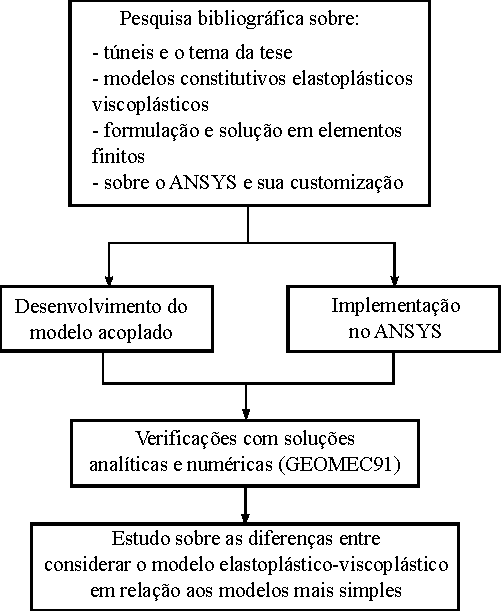
\includegraphics[scale = 1.2]{0201_2-organograma das etapas da pesquisa.pdf}
	\end{center}
	\caption{\label{organograma}Organograma das etapas da pesquisa}
\end{figure}
% ----------------------------------------------------------
\chapter{Estado da Arte}
% ----------------------------------------------------------

\section{Métodos de Escavação}

Há diversas formas de se executar túneis, tanto profundos quanto superficiais. Durante a escolha do método de escavação, o engenheiro deve levar em conta diversos fatores, tais como: geometria da seção, comprimento do túnel, condições geológicas, nível da água, restrições quanto às vibrações, estabilidade da cavidade, riscos de assentamentos superficiais, hipóteses de projeto, segurança dos operários, viabilidade ambiental e econômica. Em vista dessa complexidade é possível utilizar mais de um método de escavação ao longo do eixo do túnel. A \autoref{metodos_escavacao} resume os principais métodos de escavação.

\begin{figure}[H]
	\begin{center}
		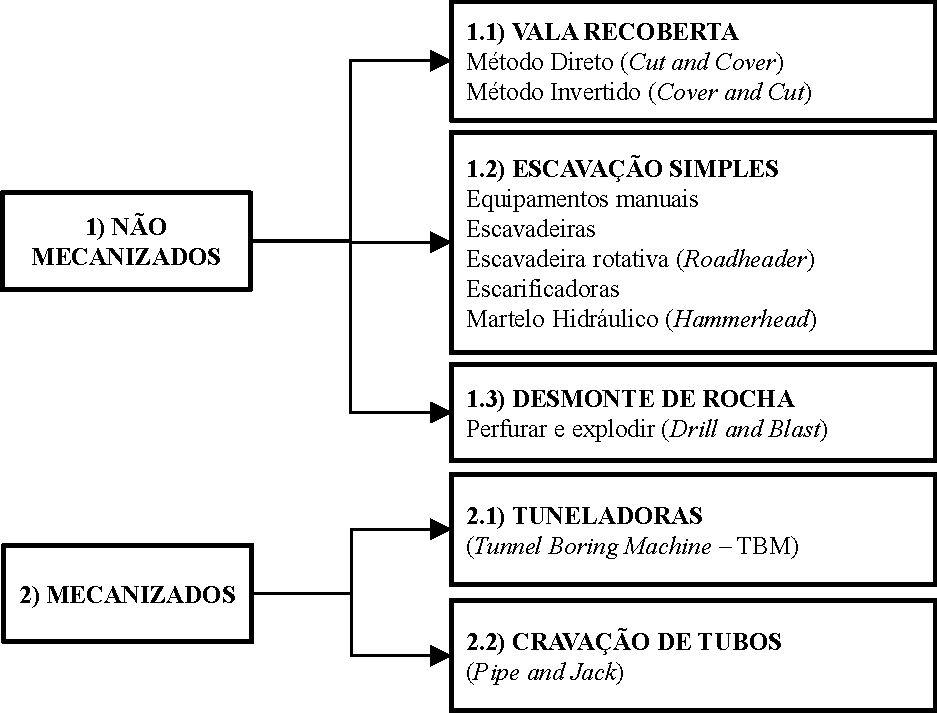
\includegraphics[scale = 1]{0301-métodos de escavação de túneis.pdf}
	\end{center}
	\caption{\label{metodos_escavacao} Métodos de escavação de túneis}
\end{figure}

Os métodos se dividem em dois grandes grupos: 1) não mecanizados (convencionais) e 2) mecanizados. A diferença é que este último é caracterizado pela presença de tuneladoras, que são máquinas especializadas em adentrar a frente de escavação. Os métodos ditos “não mecanizados”, não possuem essas máquinas especializadas, e podem ser agrupados em: vala recoberta, escavação simples e desmonte de rocha.

\subsection{Vala recoberta}

O método da vala recoberta é utilizado preferencialmente para túneis superficiais (conhecido também, nas cidades, como método a céu aberto). Pode ser executado de duas formas: direta (\textit{Cut and Cover}) ou invertida (\textit{Cover and Cut}). A \autoref{vala_recoberta} e \autoref{etapa_execucao_vala_recoberta} ilustram esse método.

\begin{figure}[H]
	\begin{center}
		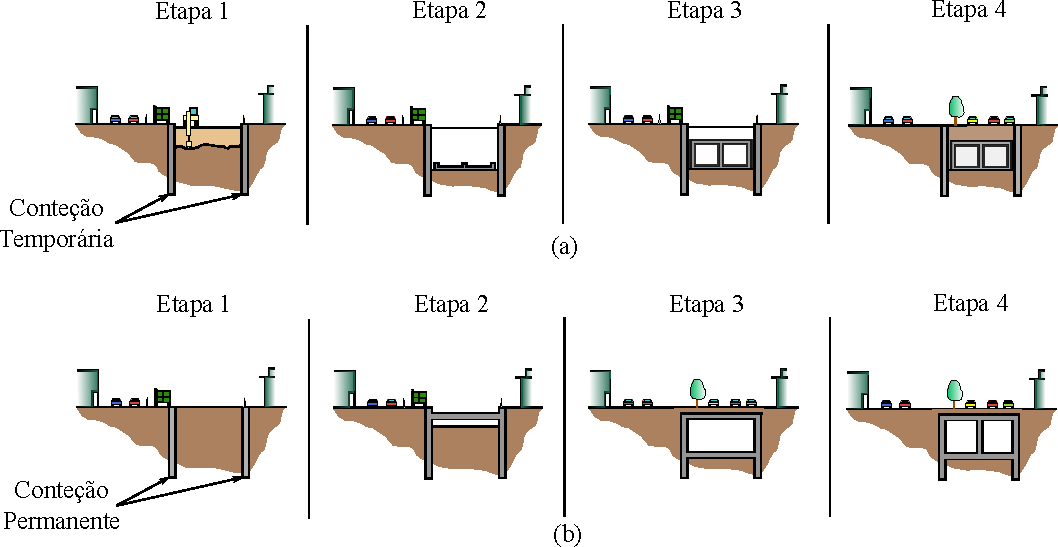
\includegraphics[scale = 0.8]{0302-vala recoberta.pdf}
	\end{center}
	\caption{\label{vala_recoberta} (a) \textit{Cut and Cover} e (b) \textit{Cover and Cut} (adaptado de: \citeonline[p. 5-2]{FederalHighwayAdministration2009})}
\end{figure}

\begin{figure}[H]
	\begin{center}
		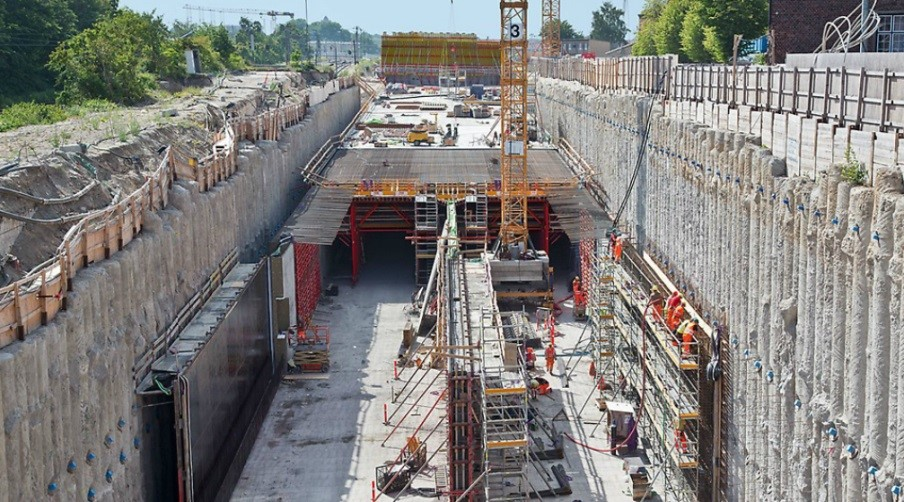
\includegraphics[scale = 1]{0303-etapa de execução pelo método de vala recoberta direta.jpg}
	\end{center}
	\caption{\label{etapa_execucao_vala_recoberta} Etapa de execução pelo método de vala recoberta direta no projeto \textit{Nordhavnsvej}, em Compenhague, Dinamarca (fonte: \citeonline[p. 1]{ROADTRAFFIC-TECHNOLOGY2019})}
\end{figure}

Como o presente trabalho está delimitado aos túneis profundos esse método de escavação estará fora do escopo desta tese. Além disso, o comportamento mecânico desse tipo de túnel é diverso dos profundos que, tal como será visto no Capítulo 4, mobilizam a resistência do maciço na estabilidade da cavidade.


\subsection{Escavação simples}


\subsection{Desmonte de rocha}

\subsection{Tuneladora}


\subsection{Cravação de tubos}



\section{Pré-suportes}



\section{Revestimento de túneis}



\section{Principais aspectos considerados em estudos numéricos recentes de túneis}





% ----------------------------------------------------------
\chapter{Comportamento Mecânico de Túneis}
% ----------------------------------------------------------

\section{Influência da escavação e o conceito de convergência da seção}

De uma forma geral, do ponto de vista do maciço, a escavação de um túnel nada mais é do que uma perturbação no seu estado natural de equilíbrio devido à remoção de parte do maciço. Essa perturbação induzirá o maciço a uma nova configuração de equilíbrio que mobilizará tensões tangenciais desviando, dessa forma, a direção das tensões principais no entorno da escavação. Através desse \textbf{arqueamento das tensões}, o próprio maciço participa da sustentação da cavidade. Esse arqueamento pode ser decomposto em dois arcos longitudinais (contidos nos planos horizontal e vertical) e um arco transversal (no plano perpendicular ao eixo do túnel), tal como mostrado na \autoref{arqueamento}.

\begin{figure}[H]
	\begin{center}
		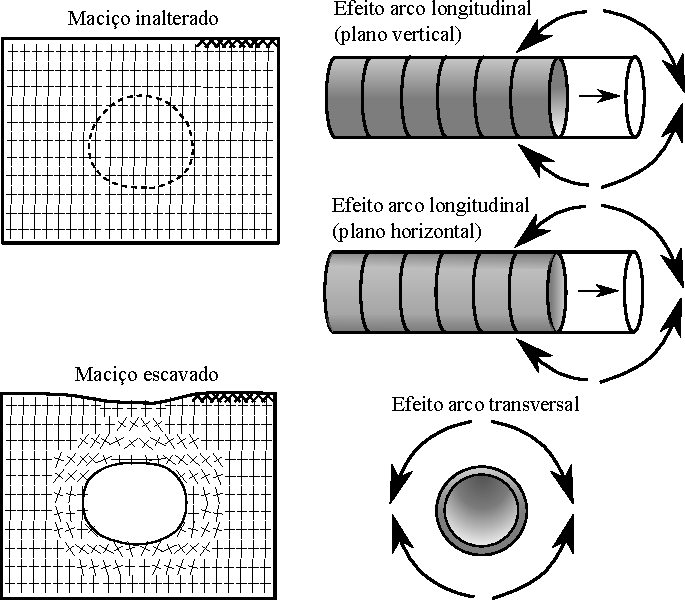
\includegraphics[scale = 1]{0401-efeito_arco.pdf}
	\end{center}
	\caption{\label{arqueamento}Ilustração do arqueamento das tensões principais (adaptado de: \citeonline[p. 10-11]{Franca2006})}
\end{figure}

A presença dos três arcos na zona que acompanha a frente de escavação faz com que essa região tenha um campo de deslocamentos tridimensional convergente em direção à face de escavação. No entanto, conforme essa frente avança e se afasta, apenas o arqueamento transversal se mantém, fazendo com que o campo de deslocamentos seja bidimensional contido no plano transversal ao eixo do túnel. Em vista disso, é conveniente caracterizar três zonas no interior do maciço: uma zona não perturbada pela escavação, uma zona de influência da frente de escavação e uma zona livre dessa influência (\autoref{campo_frente_escavacao}).

\begin{figure}[H]
	\begin{center}
		\includegraphics[scale = 1]{0402-campo vetorial de deslocamentos no maciço.pdf}
	\end{center}
	\caption{\label{campo_frente_escavacao}Campo vetorial de deslocamentos no maciço durante a escavação de um túnel (adaptado de: \citeonline[p. 12]{Franca2006})}
\end{figure}

O parâmetro geométrico mais simples e representativo do comportamento de um túnel é o fechamento de sua cavidade, também conhecido como \textbf{convergência}. Se um túnel circular estiver em um maciço homogêneo, isotrópico, submetido a um estado de tensões inicial geostático hidrostático, o campo de deslocamentos no entorno de uma seção fora da zona de influência da frente de escavação estará contido no plano transversal e será puramente radial, podendo ser expresso por uma função  $u(r)$. Nesse caso, a convergência $U$ é definida pela razão entre o deslocamento da cavidade e seu raio inicial $U=-u(r=R)/R$. A presença do sinal negativo é opcional e serve para que a convergência fique positiva se a seção diminuir, ou seja, $u(R) < 0$  (\autoref{definicao_convergencia}).

\begin{figure}[H]
	\begin{center}
		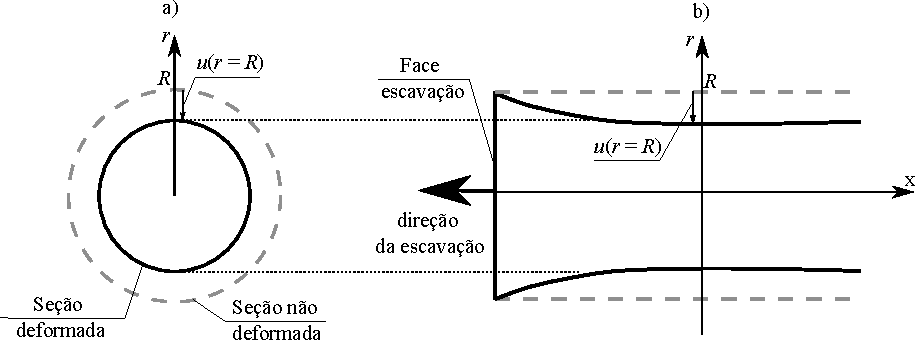
\includegraphics[scale = 1]{0403-convergencia de uma seção circular.pdf}
	\end{center}
	\caption{\label{definicao_convergencia}Ilustração das medidas geométricas que compõe a convergência de uma seção circular: a) corte transversal, b) corte longitudinal}
\end{figure}

Dependendo da anisotropia das tensões \textit{in situ} ou do formato da seção, sua deformada pode não ser radial e, na prática, podem-se usar varias medidas para compor o cálculo da convergência da seção, como exemplificado na \autoref{convergenca_secao_qualquer}.

\begin{figure}[H]
	\begin{center}
		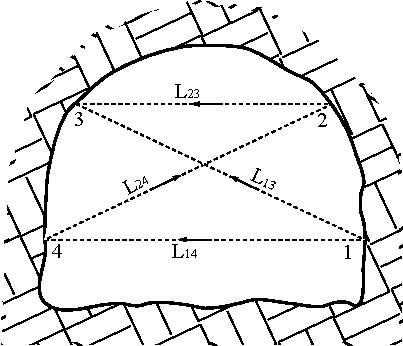
\includegraphics[scale = 1]{0404-convergencia de uma seção qualquer.pdf}
	\end{center}
	\caption{\label{convergenca_secao_qualquer}Medidas da convergência em quatro direções de uma seção não circular (adaptado de: \citeonline[p. 8]{Panet1995})}
\end{figure}

Outro aspecto importante para determinar a influência da escavação e caracterizar o comportamento global do túnel é a representação gráfica das convergências ao longo do seu eixo longitudinal, conhecida como \textbf{perfil de convergências}. Por exemplo, com o objetivo de quantificar a extensão da zona de influência da frente da escavação, Hanafy \& Emery (1980) graficaram o perfil de convergências do seu modelo de um túnel circular em um maciço homogêneo, isotrópico e elástico linear (\autoref{perfil_exemplo}).

\begin{figure}[H]
	\begin{center}
		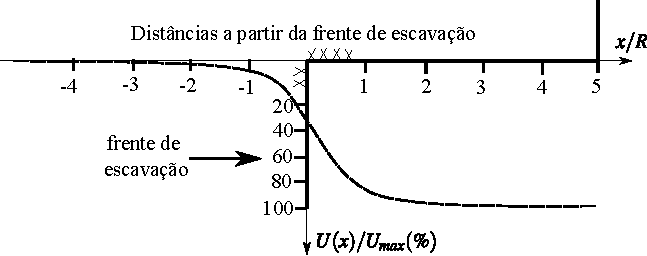
\includegraphics[scale = 1]{0405-perfil de convergencias próximo a frente de escavação.pdf}
	\end{center}
	\caption{\label{perfil_exemplo}Perfil de convergências próximo à frente de escavação (adaptado de: \citeonline{Hanafy1980} \textit{apud} \citeonline[p. 42]{Couto2011})}
\end{figure}

Como se pode ver na \autoref{perfil_exemplo}, dentro das hipóteses dos autores, a partir de cinco raios da face de escavação a convergência atinge seu valor máximo  $U_{max}$. Já na face, em $x/R=0$ , a convergência é superior à 35\% do valor máximo, sendo que a um raio de distância a convergência é de aproximadamente 80\% da total e quase 100\% se tiver ultrapassado dois raios (\citeonline{Hanafy1980} \textit{apud} \citeonline[p. 42]{Couto2011}).

\section{Mecanismos de ruptura em túneis profundos}

A execução de túneis se tornou bastante segura após os preceitos filosóficos e teóricos do método empírico NATM (\textit{New Austrian Tunneling Method}) desenvolvido por Rabcewicz (\citeyear{Rabcewicz1964a}, \citeyear{Rabcewicz1964b} e \citeyear{Rabcewicz1964c}) e \citeonline{Rabcewicz1973}. E cada vez mais os estudos numéricos vêm ajudando os projetistas na tomada de decisões seguras durante a fase de projeto e execução. Contudo, apesar dessa abordagem empírica e numérica ter diminuído significativamente o número de incidentes estes ainda existem. Compilados de acidentes podem ser encontrados em estudos da \citeonline{HealthandSafetyExecutiveHSE1996} e de pesquisadores como \citeonline{Stallmann2005}, \citeonline{Seidenfus2006} e \citeonline{Sousa2010}, tal como reunido por \citeonline{Spackova2012} na \autoref{incidentes}.

\begin{figure}[H]
	\begin{center}
		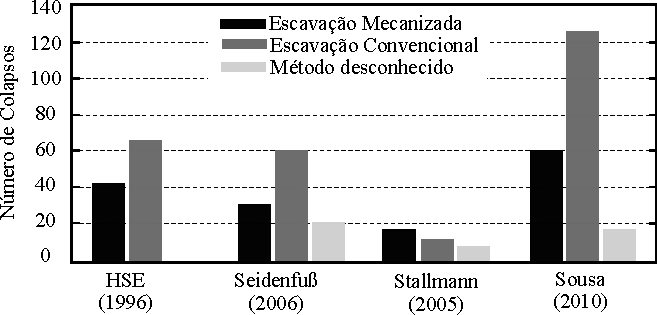
\includegraphics[scale = 1]{0406-número de incidentes em quatro banco de dados descriminado por autor e tecnologia de escavação.pdf}
	\end{center}
	\caption{\label{incidentes}Número de incidentes em quatro banco de dados descriminados por autor e método de escavação (adaptado de: \citeonline[p. 19]{Spackova2012})}
\end{figure}

\citeonline{Sousa2010}, por exemplo, agrupou os incidentes, tanto de túneis profundos como superficiais, em nove tipos, tal como apresentado na \autoref{distribuicao_incidentes}.

\begin{figure}[H]
	\begin{center}
		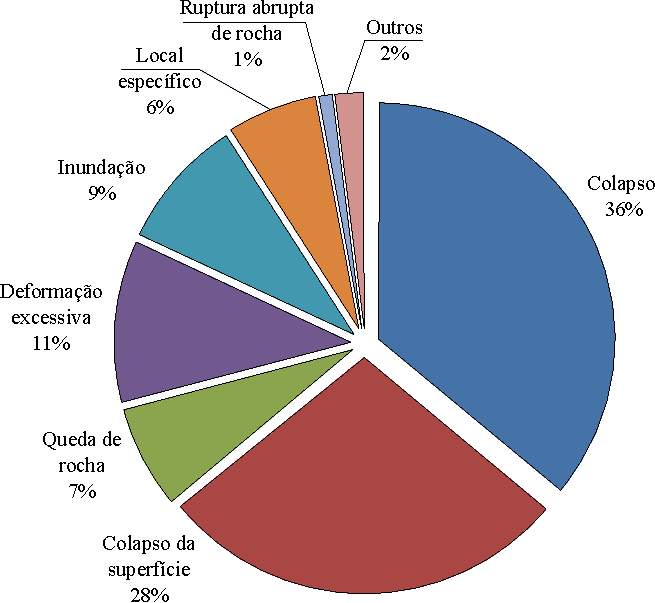
\includegraphics[scale = 1]{0407-distribuição de incidentes de acordo com nove tipologias.pdf}
	\end{center}
	\caption{\label{distribuicao_incidentes}Distribuição de incidentes de acordo com nove tipologias (adaptado de: \citeonline[p. 82]{Sousa2010})}
\end{figure}

Contudo, de forma geral, no comportamento de túneis profundos executados em maciços aparentemente contínuos, ou seja, ausência de grandes descontinuidades ou acidentes geológicos, identifica-se dois mecanismos principais de colapso (ou ruptura): \textit{Spalling} (descamação ou fragmentação) e \textit{Squeezing} (deformações excessivas diferidas no tempo).

O \textit{Spalling} é preponderante em maciço muito resistente, inicialmente pouco fraturado, no qual o nível de energia para iniciar a fissuração e consequente propagação costuma ser alto. Durante a redistribuição das tensões, causada pela escavação, as fissuras vão se desenvolvendo e destacando regiões da rocha no contorno da seção. Essas sofrem então uma descamação, ou ainda, ruptura por flambagem e tem-se, nesse último caso, uma repentina liberação de energia. Uma ruptura abrupta da rocha (\textit{rockburst}). Esse comportamento é refletido na curva tensão-deformação de uma amostra do maciço, por um significativo amolecimento após o pico de resistência, caracterizando, dessa forma, a rocha como frágil \cite[p. 83]{Kleine2007}. A \autoref{mecanismo_spalling} exemplifica esse mecanismo e a \autoref{foto_spalling} mostra a seção após tal colapso.

\begin{figure}[H]
	\begin{center}
		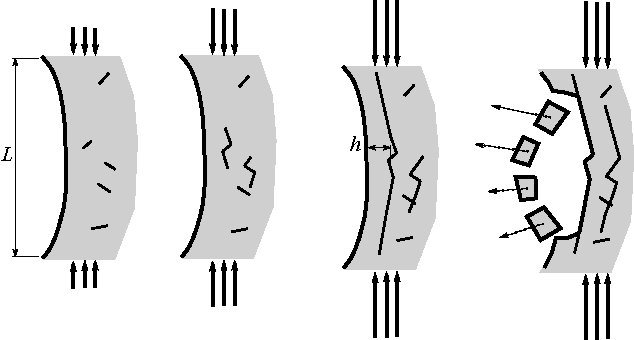
\includegraphics[scale = 1]{0408-mecanismo de ruptura do maciço próximo a seção.pdf}
	\end{center}
	\caption{\label{mecanismo_spalling}Mecanismo de ruptura por \textit{Spalling} de um comprimento $L$ junto à seção do túnel: detalhamento do crescimento das fissuras e flambagem de uma profundidade $h$ da rocha no contorno da seção (adaptado de: \citeonline[p. 267]{Germanovich2000})}
\end{figure}

\begin{figure}[H]
	\begin{center}
		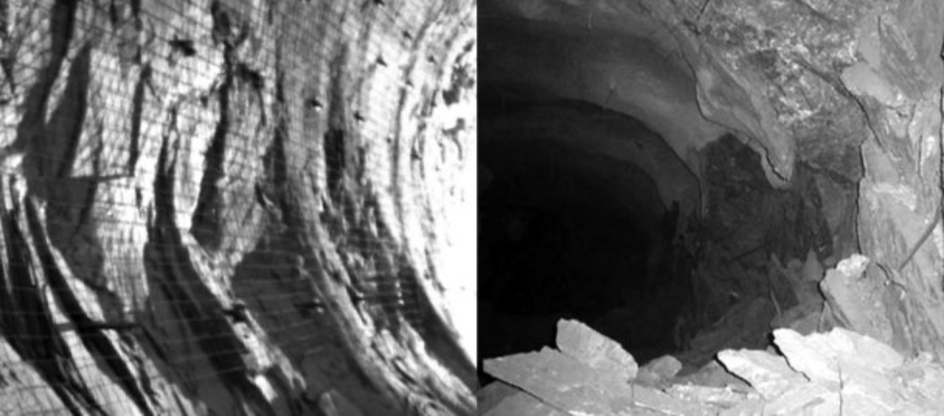
\includegraphics[scale = 1]{0409-foto ruptura por spalling.pdf}
	\end{center}
	\caption{\label{foto_spalling}À esquerda uma seção remanescente após moderada fragmentação e quebra em um túnel escavado com TBM e à direita uma seção em que parte do contorno apresentou instabilidade (flambagem) em um túnel escavado de forma não mecanizada (fonte: \citeonline[p. 1084]{Diederichs2007})}
\end{figure}

Já o \textit{Squeezing} é um modo de falha relacionado ao cisalhamento e encontrado principalmente em túneis profundos em condições de grandes tensões \textit{in situ}. Inicia-se quando a fissuração está suficientemente avançada, causando uma diminuição nas propriedades mecânicas do maciço, sem gerar instabilidade no contorno da seção. Essa diminuição das características mecânicas associada ao desenvolvimento da fissuração é progressiva e controlada, em especial, devido ao confinamento que reina no maciço. Ao contrário do primeiro mecanismo, a energia armazenada pela redistribuição das tensões é dissipada de forma gradual por deformações. Esse comportamento está intimamente relacionado com o fenômeno de fluência descrito na próxima seção a qual compreende um dos comportamentos que se pretende modelar e estudar nessa tese.

A \autoref{evolucao_convergencia} ilustra a evolução da convergência por esse fenômeno. Tal comportamento também é visto em galerias para estocagem de rejeitos radioativos em maciços argilosos profundos. Essas argilas possuem baixa condutividade hidráulica, portanto, pouca difusão molecular, sendo ideais para estocar esse material. Porém, apresentam esse comportamento diferido e que pode comprometer o projeto no longo tempo requerido para estabilização desse material radioativo. Estudos como os de \citeonline{Rousset1988} e \citeonline{Armand2013} são alguns exemplos de investigações nesse sentido. Laboratórios como o HADES na Bélgica e \textit{Meuse/Haute-Marne} (\autoref{evolucao_GED}) em Paris, são exemplos de túneis para estocagem radioativa que apresentam esse fenômeno.

\begin{figure}[H]
	\begin{center}
		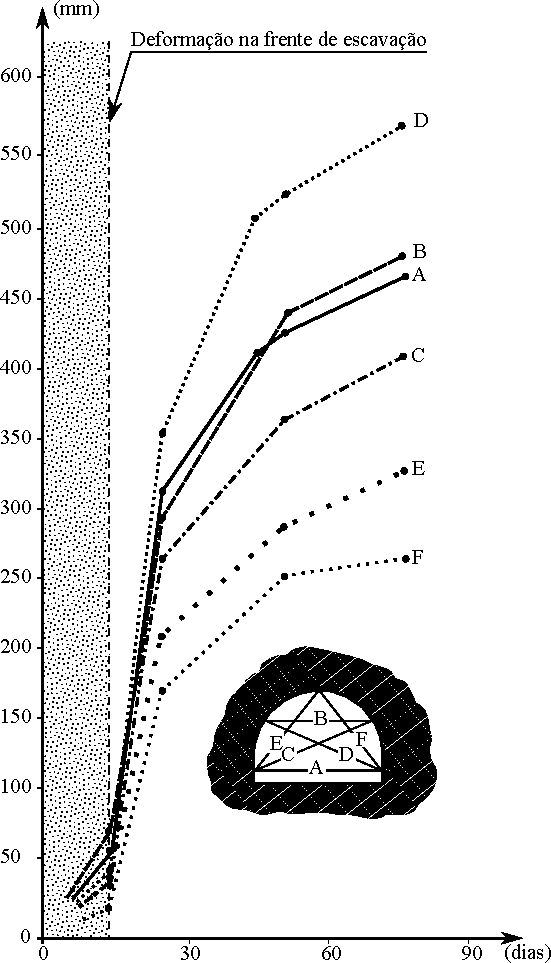
\includegraphics[scale = 1]{0410-evolução da convergencia do túnel fréjus.pdf}
	\end{center}
	\caption{\label{evolucao_convergencia}Evolução da convergência do túnel Fréjus (adaptado de: \citeonline[p. 17]{Lunardi1980})}
\end{figure}

\begin{figure}[H]
	\begin{center}
		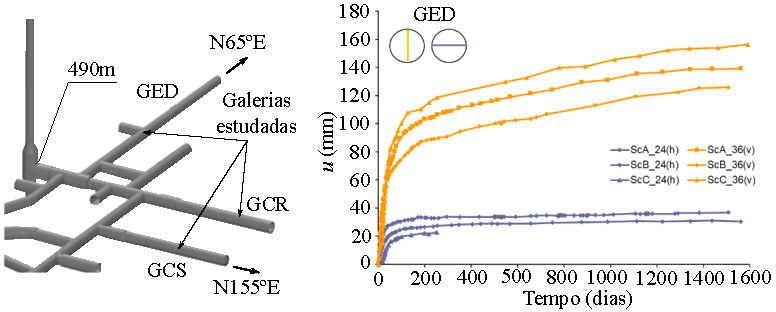
\includegraphics[scale = 1]{0411-evolucação do fechamento da seção C.pdf}
	\end{center}
	\caption{\label{evolucao_GED}Evolução do fechamento da seção GED (convergência) na galeria do laboratório \textit{Meuse/Haute-Marne}  (adaptado de: \citeonline[p. 103]{Guayacan-Carrillo2016})}
\end{figure}



\section{Influência da reologia do maciço}

\subsection{Comportamento instantâneo}

Para caracterizar o comportamento de curto prazo do maciço, o ensaio triaxial associado à medição da variação do volume é comumente utilizado. Esse ensaio clássico na mecânica das rochas permite estudar as diferentes fases do comportamento: elástica, plástica, ruptura e pós ruptura. As medidas da variação do volume permitem fazer estudos de outros aspectos do comportamento, como o coeficiente de Poisson e a dilatância. Esse ensaio, de forma resumida, consiste em submeter uma amostra cilíndrica do maciço a um estado de tensões triaxial hidrostático e, após atingido esse estado, leva-lá à ruptura através do aumento da carga axial (o desviador). \citeonline{Rousset1988}, por exemplo, caracterizou o comportamento de curto prazo de maciços argilosos profundos em frágil (argila rígida) e dúctil (argila plástica). Um maciço rígido pode ser visto na \autoref{ensaio_triaxial_rigido}.

\begin{figure}[H]
	\begin{center}
		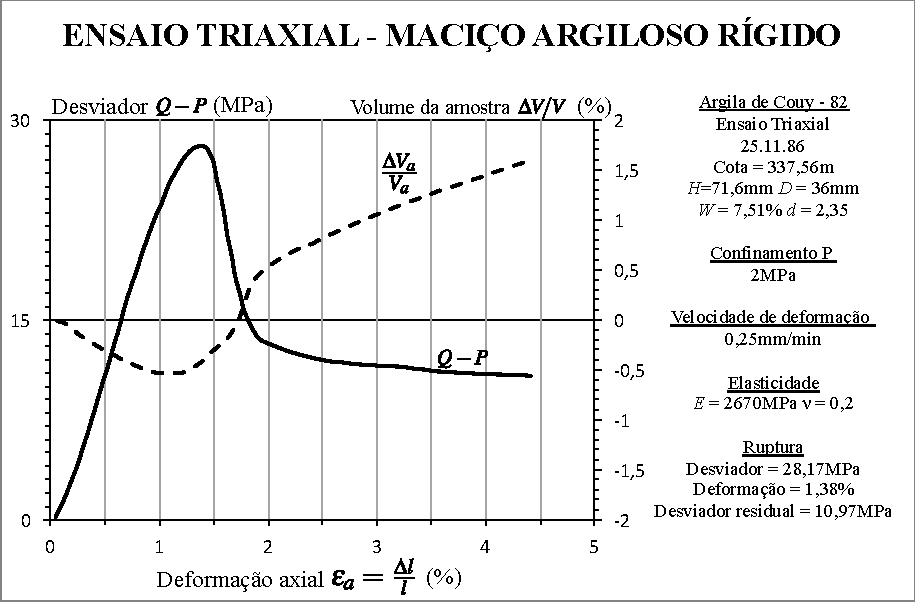
\includegraphics[scale = 0.95]{0412-ensaio triaxial argila rigida.pdf}
	\end{center}
	\caption{\label{ensaio_triaxial_rigido}Ensaio triaxial com medição da variação do volume para o caso de uma argila rígida  (adaptado de: \citeonline[p. 35]{Rousset1988})}
\end{figure}

No comportamento da \autoref{ensaio_triaxial_rigido} pode-se destacar as seguintes fases \cite[p. 34]{Rousset1988}:

\begin{alineas}
	
	\item \textbf{fase elástica} ($0\le \varepsilon \le 0,8\%$): o comportamento do maciço é linear elástico e, ao mesmo tempo, o volume da amostra diminui linearmente, os dois parâmetros elásticos, módulo de Young e Poisson, são facilmente obtidos;
	
	\item \textbf{fase pré-ruptua} ($0,8\%\le \varepsilon \le 1,3\%$): o desviador continua aumentando, mas a curva $Q-P$ não é mais linear, indicando que fenômenos irreversíveis passam a ocorrer. Ao mesmo tempo, a taxa de redução do volume diminui. Nessa fase também pode-se notar que os fenômenos irreversíveis ocorrem primeiro na curva ${\Delta V}/{V}\;$, em torno de 0,8\% da deformação enquanto o desviador é de 65\% do seu valor máximo e sua dependência ainda é linear;
	
	\item \textbf{fase de ruptura} ($1,3\%\le \varepsilon \le 1,6\%$): o desviador cai acentuadamente, o que reflete a fragilidade do comportamento dessa argila. Enquanto isso, o volume da amostra aumenta drasticamente;
	
	\item \textbf{fase pós-ruptura} ($1,6\%\le \varepsilon \le 5\%$): o desviador evoluiu pouco e mantém um valor residual de 40\% do desvio máximo. Esta resistência residual ocorre pelo atrito ao deslizamento na superfície de ruptura que apareceu durante o carregamento. Nessa fase, o volume da abertura aumenta muito, o que reflete o comportamento altamente dilatante do material (2\% superior ao volume original na deformação de 5\%).
	
\end{alineas}

Já para um maciço argiloso dúctil, o comportamento é diferente, tal como mostrado na \autoref{ensaio_triaxial_ductil}.

\begin{figure}[H]
	\begin{center}
		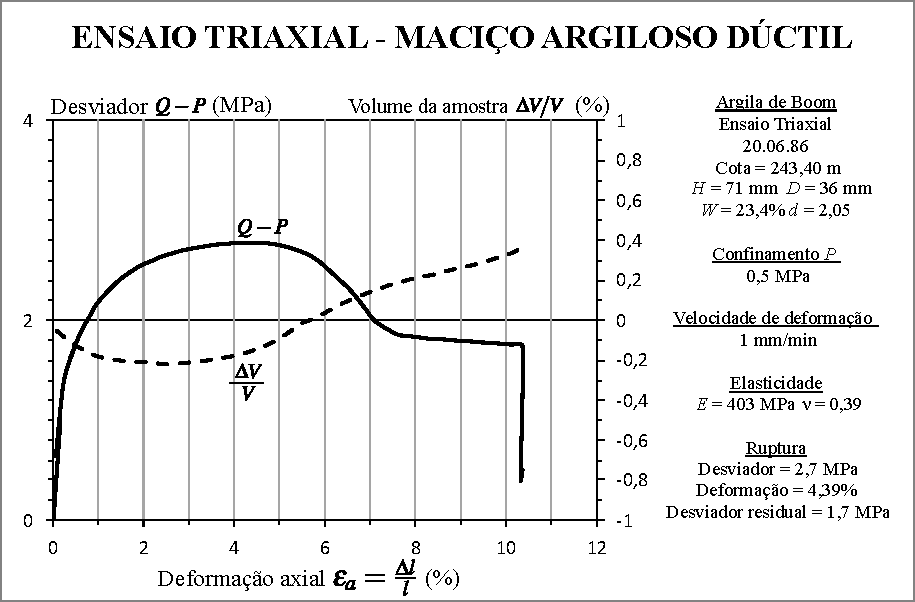
\includegraphics[scale = 0.95]{0413-ensaio triaxial argila ductil.pdf}
	\end{center}
	\caption{\label{ensaio_triaxial_ductil}Ensaio triaxial com medição da variação do volume para o caso de uma argila dúctil (adaptado de: \citeonline[p. 35]{Rousset1988})}
\end{figure}

No comportamento da \autoref{ensaio_triaxial_ductil} pode-se destacar as seguintes fases \cite[p. 35]{Rousset1988}:

\begin{alineas}
	
	\item \textbf{fase elástica} ($0\le \varepsilon \le 0,3\%$): pode-se ver que para esse caso, onde ambas as curvas são lineares, é uma fase muito pequena;
	
	\item \textbf{fase plástica com endurecimento} ($0,3\%\le \varepsilon \le 2\%$): durante essa fase o desviador continua a aumentar, mas a uma taxa decrescente. Da mesma forma, a redução do volume também teve sua taxa diminuída, mas o comportamento segue ainda de contração;
	
	\item \textbf{fase plástica perfeita} ($2\%\le \varepsilon \le 5\%$): o desviador agora segue quase constante e o volume da amostra acompanha o comportamento. Essa fase conduz a uma deformação significativa, superior a 5\%;
	
	\item \textbf{fase plástica com amolecimento} ($5\%\le \varepsilon \le 8\%$): a resistência da amostra diminui gradualmente até um platô residual e o volume começa a aumentar;
	
	\item \textbf{fase plástica residual} ($8\%\le \varepsilon \le 10\%$): o desviador é agora novamente constante, cerca de 60\% do valor máximo. O volume da amostra aumenta sensivelmente tendo uma dilatância moderada.
	
\end{alineas}

Para um maciço homogêneo, isotrópico e elástico linear a solução analítica para o campo de deslocamentos e tensões no entorno de uma seção circular afastada da zona de influência da face de escavação é conhecida desde \citeonline{Lame1852} e \citeonline{Kirsch1898}, sendo que este último generalizou a solução para um estado de tensões \textit{in situ} anisotrópico. 

Contudo, como visto nas figuras acima, a massa rochosa não é um material perfeitamente elástico e dependendo da magnitude das tensões \textit{in situ} e do desvio das tensões causada pela escavação, o túnel pode apresentar uma zona plastificada ao redor da cavidade. Quando a seção é circular, o maciço homogêneo, isotrópico, elastoplástico, com tensões iniciais geostáticas-hidrostáticas, essa zona plástica é circular e caracterizada por um raio plástico $y$. \autoref{deslocamentos_tensoes_analitico} ilustra a solução analítica de um maciço elástico e um elastoplástico. Apesar de a solução depender da forma da lei constitutiva elastoplástica, em geral, para túneis não revestidos, há uma diminuição nas tensões ao redor da cavidade e um aumento na convergência.

\begin{figure}[H]
	\begin{center}
		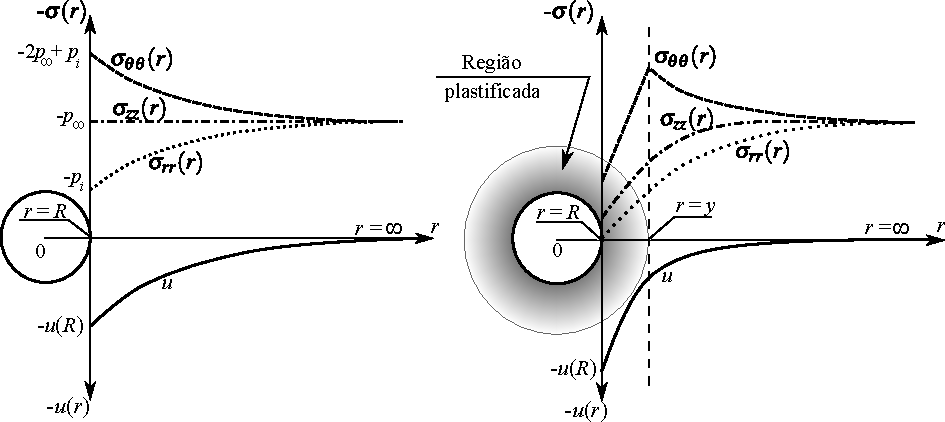
\includegraphics[scale = 1]{0414-campo de deslocamento e tensões no entorno de uma seção circular.pdf}
	\end{center}
	\caption{\label{deslocamentos_tensoes_analitico}Deslocamentos e tensões no entorno de uma seção circular submetida às tensões iniciais geostáticas-hidrostáticas $p_{\infty}$ e pressão interna $p_i$. À esquerda, maciço elástico e à direita, elastoplástico.}
\end{figure}

Algumas soluções analíticas considerando leis elastoplásticas específicas para túneis não revestidos podem ser encontradas, por exemplo, em \citeonline{Salencon1969}, \citeonline{Hoek1980}, \citeonline{Brown1983}, \citeonline{Detournay1987}, \citeonline{Carranza-Torres1999}, \citeonline{Carranza-Torres2004}, Sharan (\citeyear{Sharan2003,Sharan2005}) e \citeonline{Alejano2009}.

Um dos objetivos desta tese é justamente implementar um algoritmo geral para considerar esse comportamento instantâneo elastoplástico conjuntamente com o fenômeno diferido no tempo.

\subsection{Comportamento diferido no tempo}

O comportamento viscoso do maciço, caracterizado pela deformação contínua no tempo, mesmo sobre tensão e temperatura constantes, é denominado \textbf{fluência} (\textit{Creep}). E ocorre devido aos deslizamentos, quebras e acomodações no interior do maciço e, também, em conjunto com transporte e difusão de massa fluída. Em solos argilosos com condições drenadas, parte da fluência é dada conjuntamente com a dissipação de poro-pressão. Em maciços rochosos, com pouca umidade, essa condição está bastante relacionada com o avanço de trincas e fissuras sobre grande confinamento. Esse comportamento é geralmente caracterizado através de um ensaio triaxial de fluência com uma amostra do maciço. Nesse teste, sobre condições de temperatura e umidade controladas, registram-se as deformações axiais da amostra temporalmente, mantendo-se uma pressão hidrostática e um dado desviador constante. Dessa forma, tem-se a curva típica apresentada na \autoref{curva_caracteristica_fluencia}.

\begin{figure}[H]
	\begin{center}
		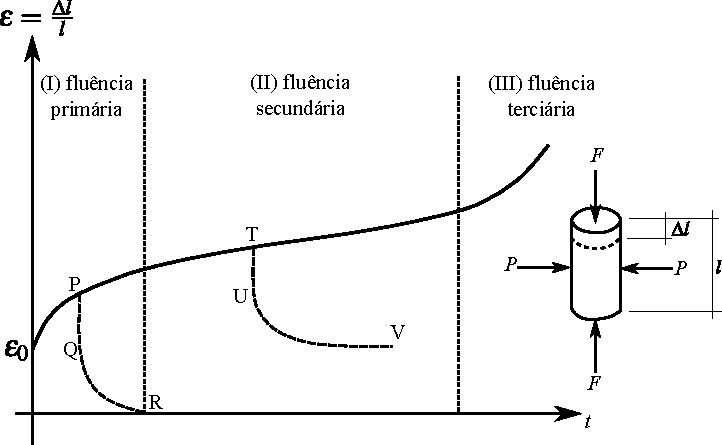
\includegraphics[scale = 1]{0415-curva característica de um ensaio de fluência com os três estágios de comportamento.pdf}
	\end{center}
	\caption{\label{curva_caracteristica_fluencia}Curva característica em um ensaio de fluência com os três estágios de comportamento (adaptado de: \citeonline[p. 107]{Costa1984})}
\end{figure}

Conforme pode-se ver na figura acima, no instante de aplicação da carga axial o corpo de prova sofre uma deformação instantânea inicial $\varepsilon_0$ elástica ou, dependendo do nível das tensões, elastoplástica. Conforme o tempo avança as deformações continuam aumentando, porém, a uma taxa decrescente. Esse estágio é chamado de \textbf{fluência primária} (ou transiente), pois em seguida a taxa de deformação diminui até ficar constante iniciando dessa forma o segundo estágio chamado de \textbf{fluência secundária} (permanente ou estacionária). Após essa fase, que pode consumir a maior parte do tempo, as deformações podem evoluir para o terceiro estágio chamado de \textbf{fluência terciária} (instável), onde a taxa de deformação passa a aumentar até que o material atinge a ruptura \cite{Costa1984}. Contudo, dependendo do nível das tensões, nem sempre a amostra apresenta os três estágios, podendo, inclusive, haver uma estabilização das deformações no tempo.

Além desses estágios de comportamento citados, a recuperação das deformações é outro fenômeno característico de materiais em regime de fluência. Se durante a fluência primária for retirado a carga $F$ o corpo recuperará a sua configuração original seguindo a trajetória $\overline{\textrm{PQR}}$, sendo o trecho $\overline{\textrm{PQ}}$ uma recuperação rápida e instantânea e o trecho $\overline{\textrm{QR}}$ uma recuperação lenta, assintótica e completa (salvo se houverem deformações plásticas durante o carregamento). Nesse caso, em que a recuperação é completa, o maciço está em regime viscoelástico. Contudo, se a descarga for feita no segundo estágio, haverá o mesmo comportamento instantâneo (trecho $\overline{\textrm{TU}}$) e assintótico (trecho $\overline{\textrm{UV}}$), mas a recuperação pode não ser mais completa. Nesse caso, evidencia-se o material comportando-se em seu regime viscoplástico \cite{Costa1984}. Um exemplo típico desse ensaio pode ser visto na \autoref{curva_caracteristica_fluencia_ensaio}.

\begin{figure}[H]
	\begin{center}
		\includegraphics[scale = 1]{0416-ensaio triaxial de fluência da Argila de Boom.pdf}
	\end{center}
	\caption{\label{curva_caracteristica_fluencia_ensaio}Ensaio triaxial de fluência da Argila de Boom (adaptado de: \citeonline[p. 42]{Rousset1988})}
\end{figure}

Na figura acima, pode-se destacar as seguintes fases \cite[p. 42]{Rousset1988}:

\begin{alineas}
	
	\item para um pequeno desviador (1,75MPa) a deformação aumenta rapidamente no início. Sua evolução, em seguida, diminui e se estabiliza depois de alguns dias. Nessa etapa foi observado apenas a fase primária, transiente;
	
	\item para um desviador moderado (2,25MPa), após uma fase rápida, mas desacelerada (fase primária), observa-se o desenvolvimento de uma fase com taxa de deformação constante ($\dot{\varepsilon}\simeq 7\cdot {{10}^{-6}}{{h}^{-1}}$). Essa é uma fase de fluência secundária, que leva a deformações relativamente importantes, da ordem de 3,5\% após três meses;
	
	\item para um desviador forte (2,75MPa), próximo do limite máximo de resistência do comportamento instantâneo (\autoref{ensaio_triaxial_ductil}), a taxa de deformação da fase secundária é cinco vezes maior do que a anterior. Após duas semanas, leva a um aumento na taxa de deformação (fase terciária) e, finalmente, a ruptura da amostra, logo que a deformação ultrapassa 6\%.
	
\end{alineas}

Como pode-se ver na \autoref{curva_caracteristica_fluencia_ensaio}, o ensaio de fluência permite conhecer os diferentes limiares que separam os diferentes comportamentos viscosos: fluência primária, secundária, secundária com terciária seguida de ruptura. Permite também estimar a velocidade de fluência durante a fase secundária, dependendo da magnitude do desviador. Dessa forma, pode-se obter os principais parâmetros de viscosidade para o modelo do material. Cabe salientar que a fluência depende da interação entre fatores intrínsecos do maciço (como a forma, defeitos e composição da micro e macroestrutura) com fatores extrínsecos (como a magnitude da tensão desviadora, temperatura, pressão de confinamento e umidade). Portanto, os ensaios devem simular esses fatores externos de modo a obter parâmetros para uma correta modelagem.

Maiores detalhes sobre ensaios de fluência e caracterização desse comportamento podem ser obtidos em \citeonline{Rousset1988}, particularmente para maciços argilosos profundos, e ainda em \citeonline{Feda1992}, \citeonline{Hunsche1994}, \citeonline{Dusseault1993} e \citeonline{Cristescu1998}.

Portanto, no comportamento do túnel, além da deformação instantânea (resultante da redistribuição das tensões e consequente plastificação do maciço ao redor da cavidade), deformações diferidas podem ocorrer e, dado a magnitude dos efeitos, pode tender a estabilização ou levar o sistema maciço-revestimento a danos e colapso. De forma ilustrativa, a \autoref{evolucao_U_t_x} mostra a convergência $U$ em função do tempo $t$ e do avanço da escavação $x$ para uma dada seção.

\begin{figure}[H]
	\begin{center}
		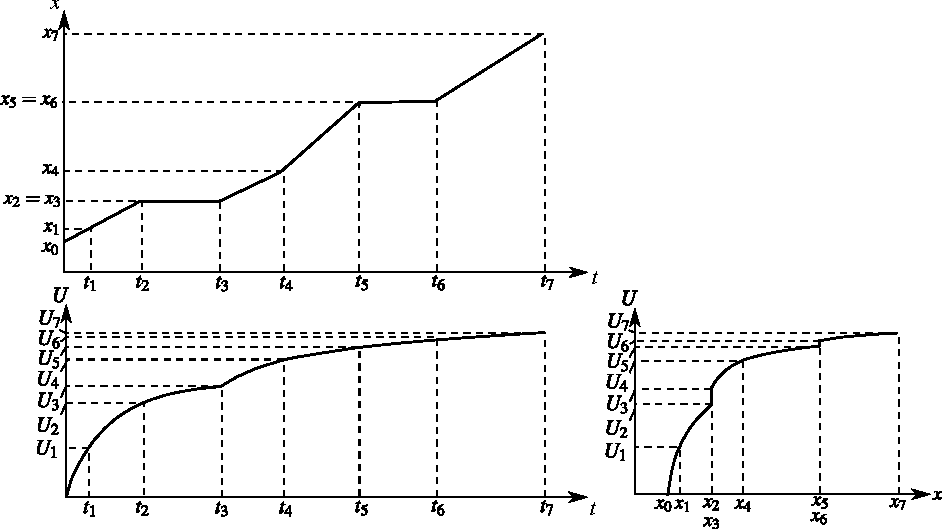
\includegraphics[scale = 1]{0417-evolução da convergência U no tempo t em função do avanço da escavação.pdf}
	\end{center}
	\caption{\label{evolucao_U_t_x}Evolução da convergência $U$ no tempo $t$ em função do avanço da escavação $x$ (adaptado de: \citeonline[p. 8]{Panet1995})}
\end{figure}

Como pode-se ver na figura acima, mesmo sem escavar nos intervalos $[t_2,t_3]$ e $[t_5,t_6]$ a convergência não é constante, tal como seria em um maciço apenas elástico ou elastoplástico. Nesse caso ilustrativo, a convergência não só evoluiu como também se estabilizou com o tempo. 

Há diversas formas de introduzir esse comportamento no interior das análises de túneis. Nas soluções analíticas e numéricas, diversas leis constitutivas são empregadas. Pode-se classificar essas leis como: 

\begin{alineas}
	
	\item \textbf{empírico-experimentais}: geralmente são leis expressas por funções ajustadas empiricamente. Para tal existem funções potenciais, como em \citeonline{Obert1965}, exponeciais em \citeonline{Singh1968} e hiperbólicas como em \citeonline{Mesri1981} e \citeonline{Phienwej2007};
	
	\item \textbf{acoplamento hidro-mecânico}: leis que consideram o maciço como sendo constituído por uma fase sólida e fluída. Exemplos dessa abordagem podem ser encontrados nos trabalhos de \citeonline{Griffiths1994}, \citeonline{Leem1999}, \citeonline{Wong2008}, \citeonline{Deleruyelle2014} e \citeonline{Prassetyo2018}.
	
	\item \textbf{Viscoelásticas}: leis formuladas através da analogia com sistemas mecânicos derivados da associação de elementos simples (mola e amortecedor). Estudos com essa abordagem podem ser encontrados em \citeonline{Sakurai1978}, \citeonline{Panet1979}, \citeonline{Sulem1987}, \citeonline{Ladanyi1988}, \citeonline{Goodman1989}, Pan e Dong (\citeyear{Pan1991a}, \citeyear{Pan1991b}), \citeonline{Fahimifar2010}, \citeonline{Wang2014} e \citeonline{Wang2018};
	
	\item \textbf{Viscoplásticas}: leis formuladas através da teoria da plasticidade dependente do tempo, que, tal como as leis viscoelásticas, também possuem uma analogia com sistemas mecânicos elementares, mas introduzem um elemento de atrito, para representar o ponto a partir do qual o fenômeno passa a ter importância. Leis desse tipo podem ser encontradas nos estudos de \citeonline{Berest1983}, \citeonline{Fritz1984}, Cristescu (\citeyear{Cristescu1985}, \citeyear{Cristescu1988}), \citeonline{Ottosen1986}, \citeonline{Bernaud1991}, \citeonline{Gioda1994}, \citeonline{Boidy2002}, \citeonline{Sekine2009} e Roate\c{s}i (\citeyear{Roatesi2012},\citeyear{Roatesi2014}).
	
\end{alineas}

Um exemplo da magnitude dos efeitos viscosos frente a leis elásticas e elastoplásticas em túneis profundos, pode ser vista no perfil de convergências da \autoref{perfil_convergencias_sterpi} obtidas de análises em axissimetria. Quando se considera no modelo apenas a lei elastoviscoplástica em regime secundário, tal possui um comportamento intermediário entre as leis elásticas e elastoplásticas. Além disso, quanto mais rápido a escavação, mais a resposta se aproxima da solução em elasticidade e quanto mais lenta mais se aproxima da elastoplasticidade. Isso é uma característica própria dos modelos viscoplásticos, por exemplo.

\begin{figure}[H]
	\begin{center}
		\includegraphics[scale = 1]{0418-perfil de convergências.pdf}
	\end{center}
	\caption{\label{perfil_convergencias_sterpi}Perfil de convergências, em análises numéricas axissimétricas com maciço elástico (EL), elastoplástico (EP), viscoelástico (VE), viscoplástico com fluência no regime secundário (VP) e em regime terciário (VP3), todos na ausência de revestimento (adaptado de: \citeonline[p. 329]{Sterpi2009})}
\end{figure}

Outra abordagem é a combinação de diversos comportamentos, tanto instantâneos quanto diferidos. Esse é o principal enfoque dessa tese, que compreenderá a implementação de um comportamento elastoplástico-viscoplástico.

\subsection{Alguns estudos considerando leis elastoplásticas e viscoplásticas}

Alguns estudos considerando leis elastoplásticas-viscoplásticas podem ser encontrados em Rousset (\citeyear{Rousset1988}, \citeyear{Rousset1990}), \citeonline{Piepi1995}, \citeonline{Purwodihardjo2005}, \citeonline{Kleine2007}, \citeonline{Shafiqu2008}, \citeonline{Debernardi2009}, \citeonline{Souley2011}, \citeonline{Manh2015} e \citeonline{Vrakas2015}. A seguir alguns comentários sobre cada um desses estudos.

\textbf{\citeonline{Rousset1988}}, no intuito de estudar túneis em maciços argilosos profundos (usados para estocagem de rejeitos radioativos) fez um excelente trabalho de caracterização experimental do comportamento desses e classificou-os em rígidos e dúcteis. Propôs um modelo elastoplástico-viscoplástico com critério tanto de Tresca quanto Mohr-Coulomb, perfeito (para as argilas rígidas) e com amolecimento bi-linear (para as dúcteis). O modelo de \citeonline{Perzyna1966} foi adotado como sendo o mecanismo viscoso com as mesmas superfícies de escoamento da elastoplasticidade. O seu trabalho compreende principalmente soluções analíticas.

Seguindo os mesmos passos de Rousset, \textbf{\citeonline{Piepi1995}} estudando argilas rígidas, desenvolveu um cálculo semi-analítico para um túnel circular em um maciço elastoplástico-viscoplástico com critério de Tresca sem endurecimento ou amolecimento. Também, no mesmo trabalho implementou essa lei constitutiva (entre outras como von-Mises, Drucker-Prager e Mohr-Coulomb) em elementos finitos, para abordar túneis em axissimetria, calibrou os parâmetros através de ensaios e verificou os resultados com sua solução analítica.

\textbf{\citeonline{Purwodihardjo2005}}, apresentam o modelo elastoplástico-viscoplástico composto pelo modelo elastoplástico CJS desenvolvido por \citeonline{Cambou1987}, que, além de dividir o mecanismo em uma parcela volumétrica e desviatória, leva em conta a dependência da densidade do maciço através da teoria do estado crítico, como pode-se ver em \citeonline{Maleki2000}. A parcela diferida é dada pelo modelo viscoplástico de \citeonline{Perzyna1966} com o parâmetro de viscosidade em função da distância entre o estado de tensões e a superfície de ruptura, para representar a fase terciária. O critério viscoplástico é inspirado na teoria da superfície delimitadora de \citeonline{Kaliakin1990}. O modelo foi calibrado com os ensaios triaxiais feitos por \citeonline{Piepi1995}. Por fim, seu modelo foi utilizado para analisar um estudo de caso referente ao túnel de \textit{Tartaiguille}, localizado entre \textit{Valence} e \textit{Montélimar} (França), utilizando análises axissimétricas e em estado plano de deformações.

\textbf{\citeonline{Kleine2007}} propõe um novo modelo reológico chamado de L\&K (Laigle \& Kleine) para prever o comportamento a curto, médio e longo prazo de maciços rochosos. Esse modelo é baseado no modelo CJS com o critério de plasticidade de Hoek-Brown. A parcela diferida também é dada por um modelo viscoplástico de \citeonline{Perzyna1966} não associado. É aplicado em dois estudos de caso: do laboratório de pesquisas nucleares canadense da AECL (\textit{Atomic Energy of Canada Limited}) localizado no interior do granito \textit{Lac du Bonnet}, e da galeria GMR do laboratório \textit{Meuse/Haute-Marne}.

\textbf{\citeonline{Shafiqu2008}} incorporaram o modelo elastoplástico-viscoplástico de \citeonline{Kaliakin1990} e \citeonline{Kaliakin2005} em um programa de elementos finitos escrito em \textit{Fortran90} para análise bidimensional (estado plano de deformações e axissimetria) do túnel contratado N-2 para o Projeto da estação de tratamento de água no nordeste da península de San Francisco. Também modelaram a dissipação da poropressão através de uma versão da equação matricial de \citeonline{Biot1941} dada por \citeonline{Lewis1998}. Chegaram à conclusão que o modelo elástico subestima os deslocamentos no revestimento quando comparado com aqueles previstos pelo seu modelo elastoplástico-viscoplástico.

\textbf{Barla, Bonini e Debernardi (\citeyear{Barla2008}, \citeyear{Barla2010})} comparam os resultados de três modelos: dois modelos numéricos elastoplástico-viscoplástico (CVISC nativo do software FLAC2D, conforme \citeonline{ITASCA2006} e SHELVIP desenvolvido por \citeonline{Debernardi2008}) e um elastoviscoplástico analítico (VIPLA desenvolvido por \citeonline{Lemaitre1994}). Essa comparação é feita em relação ao acesso de \textit{Saint Martin La Porte} (no túnel de Base \textit{Lyon-Turin}) em análises de deformação plana e axissimétricas. A ênfase desses pesquisadores estava na aplicação do modelo mais recente SHELVIP que compreende uma superfície de plasticidade sem lei de endurecimento/amolecimento e uma superfície viscoplástica com endurecimento. Mais tarde, \citeonline{Debernardi2009}, seguiram desenvolvendo esse modelo apresentando soluções analíticas.

\textbf{\citeonline{Souley2011}} apresentam o desenvolvimento de um modelo para prever o comportamento instantâneo e diferido do maciço argiloso \textit{Callovo-Oxfordian} onde se encontra o laboratório subterrâneo para estocagem radioativa \textit{Meuse/Haute-Marne} em Paris. A resposta instantânea é assumida como elastoplástica com superfície de plasticidade de Hoek-Brown e apresenta endurecimento/amolecimento. Já o comportamento diferido é baseado no modelo de Lemaitre modificado proposto por \citeonline{Su2007}. Após calibrar esse modelo com ensaios triaxiais de laboratório, partem para aplicação da galeria GED que possui tensão \textit{in situ} horizontal e vertical diferentes. Contudo, tal como apontado pelos autores do estudo, seu modelo subestimou os valores das convergências verticais e superestimou as horizontais.

\textbf{\citeonline{Manh2015}}, utilizaram o modelo CVISC, cuja formulação pode ser encontrada em \citeonline{Bonini2009}, para simular o comportamento diferido anisotrópico da galeria de acesso \textit{Saint Martin La Port} (no túnel de Base \textit{Lyon-Turin}). Nesse modelo, a componente volumétrica é modelada utilizando um comportamento puramente elastoplástico com função de escoamento de Mohr-Coulomb e, na componente desviadora, o mesmo modelo elastoplástico associado com o modelo reológico de Burger (Kelvin associado com Maxwell). Esses autores também apresentam uma solução analítica em estado plano de deformações para esse modelo considerando uma seção circular, maciço homogêneo, incompressível e tensões geostáticas-hidrostáticas. Mais tarde \citeonline{Mata2018} aplicou esse mesmo modelo no estudo de caso do túnel rodoviário \textit{Fréjus} e sua galeria de segurança. Comparando o método de escavação com perfuração e detonação com TBM, viu que este ultimo reduz significativamente as deformações no longo prazo.

\textbf{\citeonline{Vrakas2015}} desenvolveram uma função hiperbólica para corrigir a convergência obtida em soluções que consideram pequenas deformações, eliminando assim a necessidade de análises em grandes deformações (para túneis cujas convergências excedem 10\% do raio do túnel) que estão associadas com o comportamento diferido no tempo.

\textbf{\citeonline{Kargar2019}} apresenta soluções analíticas para alguns modelos viscoelásticos e o modelo CVISC.

\section{Influência da forma da seção}

Muitas análises consideram, por simplificação, a seção circular. Esse formato de seção com um estado inicial de tensões geostático-hidrostático em um maciço homogêneo e isotrópico, fora da zona de influência da face de escavação, garante um campo de deslocamentos puramente radial. Essas condições são particularmente comuns nas soluções analíticas que consideram estado plano de deformações. Contudo, seções diferentes das circulares apresentam um campo de tensões e deformações não uniformes, havendo concentração de tensões próximo às quinas. Isso pode ser visto na \autoref{trajetorias_hoekbrown}.

\begin{figure}[H]
	\begin{center}
		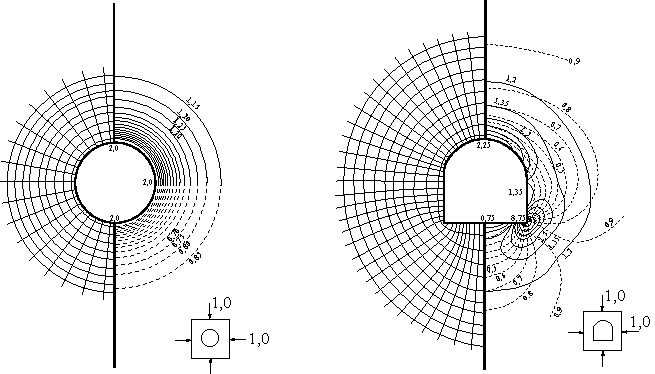
\includegraphics[scale = 1.3]{0419-trajetória das tensões principais.pdf}
	\end{center}
	\caption{\label{trajetorias_hoekbrown}Trajetória das tensões principais e linhas de isotensão, da maior e menor tensão principal, para seção circular (à esquerda) e ferradura (à direita) em condições geostáticas hidrostáticas (adaptado de: \citeonline[p. 469, 484]{Hoek1980})}
\end{figure}

\section{Influência da profundidade do túnel}

A profundidade do túnel está diretamente relacionada com o estado de tensões iniciais. Dados empíricos (\autoref{coeficiente_empuxo}a) sugerem que a tensão vertical pode ser estimada através da seguinte expressão \cite[p. 96]{Hoek1980}:

\begin{equation}
	\sigma_v(z=H)= \gamma H ,
\end{equation}

em que $\gamma$ é o peso específico do maciço e $H$ a profundidade do túnel. \citeonline{Hoek1980} reunem diversos dados que indicam que $\gamma$ (para maciços rochosos) situa-se na faixa de 20kN/m³ à 30kN/m³. Contudo, esses limites podem variar dependendo do banco de dados utilizado como, por exemplo, em \citeonline[p. 1030]{Martin2003}.

\begin{figure}[H]
	\begin{center}
		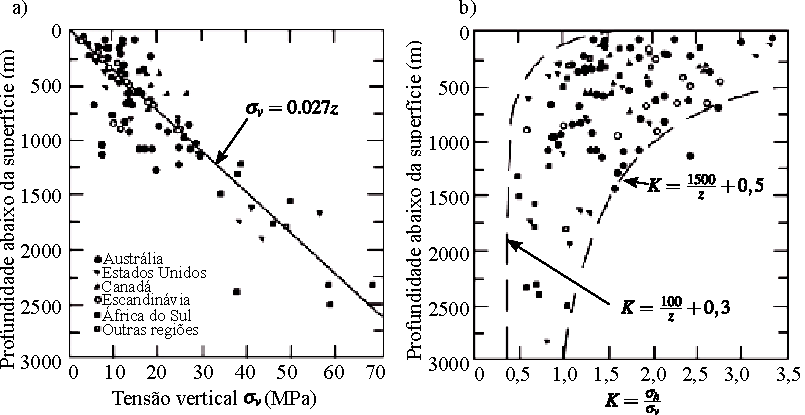
\includegraphics[scale = 1.0]{0420-tensoes verticais e coeficiente de empuxo k.pdf}
	\end{center}
	\caption{\label{coeficiente_empuxo}a) tensões verticais e b) razão entre a tensão horizontal e vertical (coeficiente de empuxo $K$)  (adaptado de: \citeonline[p. 99-100]{Hoek1980})}
\end{figure}

Como pode ser visto na \autoref{coeficiente_empuxo}b, há certa dispersão da tensão horizontal. Esse aspecto ainda hoje é objeto de estudo e uma boa revisão desses trabalhos pode ser obtido em \citeonline{Zhu2013}. Muitos desses trabalhos propõem equações simplificadas para obter o valor do coeficiente de empuxo $K$. Por exemplo, \citeonline[p. 32]{Sheorey1994} desenvolveu um modelo elasto-estático termal para as tensões na crosta da terra e obteve a seguinte equação simplificada que pode ser utilizada para estimar o coeficiente de empuxo $K$ em maciços rochosos:

\begin{equation}
	K = 0,25 + 7E_h(0,001+1/H).
\end{equation}

Sendo $H$ (m) a profundidade e $E_h$ (GPa) o módulo de deformação médio horizontal na parte superior da crosta terrestre. Contudo, como apontado por Sheorey, seu trabalho não explica a ocorrência de tensões verticais mais altas do que a profundidade indicaria ou o porquê de duas tensões horizontais raramente serem iguais. Segundo \citeonline[p. 67]{Hoek1998}, essas diferenças provavelmente se devem às características topográficas e geológicas locais, que não podem ser consideradas em um modelo de grande escala. Consequentemente, onde as tensões \textit{in situ} tendem a ter uma influência significativa no comportamento de aberturas subterrâneas é melhor medi-las \textit{in loco}.

Para túneis profundos, quando $H/D > 10$ , sendo $D$ o diâmetro equivalente da seção, é comum durante as análises, desprezar-se a variação da tensão vertical com a profundidade. Uma vez que, em túneis profundos, a variação de tensão ao longo do diâmetro da seção é irrelevante frente a magnitude da tensão na cota da profundidade, ou seja,

\begin{equation}
	\left|\Delta\sigma_v\right| = \left| \sigma_v(H+D/2)-\sigma_v(H-D/2)\right| = \left| \sigma_v(D) \right| <<  \left| \sigma_v(H)\right|.
\end{equation}

Esse princípio pode ser melhor entendido através da \autoref{tunel_profundo}.

\begin{figure}[H]
	\begin{center}
		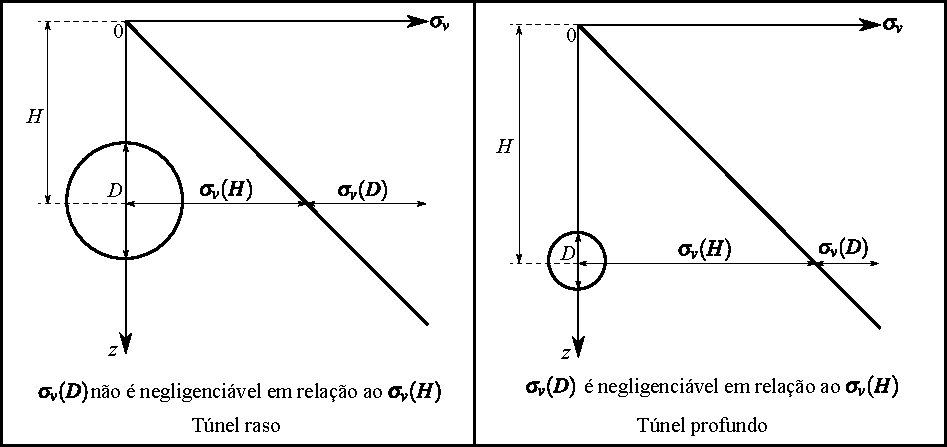
\includegraphics[scale = 1.0]{0421-tunelprofundo.pdf}
	\end{center}
	\caption{\label{tunel_profundo}Princípio para se desconsiderar a variação da tensão vertical na região próxima ao túnel  (adaptado de: \citeonline[p. 8]{Benamar1996})}
\end{figure}

De qualquer forma, conforme a \autoref{coeficiente_empuxo}, a consideração das tensões iniciais geostática hidrostática é apenas um caso específico de tensões \textit{in situ}, ou seja, quando $K=1$. A diferença entre as tensões verticais e horizontais afetam fortemente o campo de tensões e deformações após a escavação. Isso pode ser visto em análises elásticas com estado plano de deformações através, por exemplo, da comparação entre a \autoref{trajetorias_hoekbrown} e a \autoref{trajetorias_hoekbrown_aniso} obtidas por \citeonline{Hoek1980}.

\begin{figure}[H]
	\begin{center}
		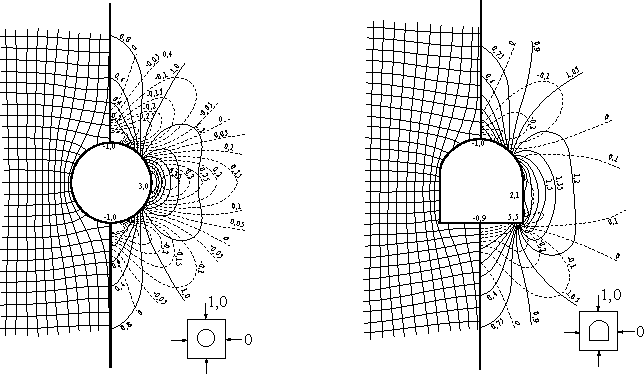
\includegraphics[scale = 1.3]{0422-trajetória das tensões principais_aniso.pdf}
	\end{center}
	\caption{\label{trajetorias_hoekbrown_aniso}Trajetória das tensões principais e linhas de isotensão da maior e menor tensão principal para seção circular (à esquerda) e ferradura (à direita) considerando $K=0$  (adaptado de: \citeonline[p. 468,483]{Hoek1980})}
\end{figure}

Além disso, quando o maciço apresenta um comportamento elastoplástico, a anisotropia das tensões \textit{in situ} afeta o formato da zona de plastificação. Isso pode ser visto no estudo de \citeonline{Detournay1988}. Utilizando soluções analíticas para seções circulares em um maciço elastoplástico com lei do comportamento de Mohr-Coulomb, esses autores apresentam um ábaco identificando os \textbf{modos de falha} (formas das zonas de plastificação) de acordo com o grau de anisotropia das tensões iniciais (\autoref{modos_falha}).

\begin{figure}[H]
	\begin{center}
		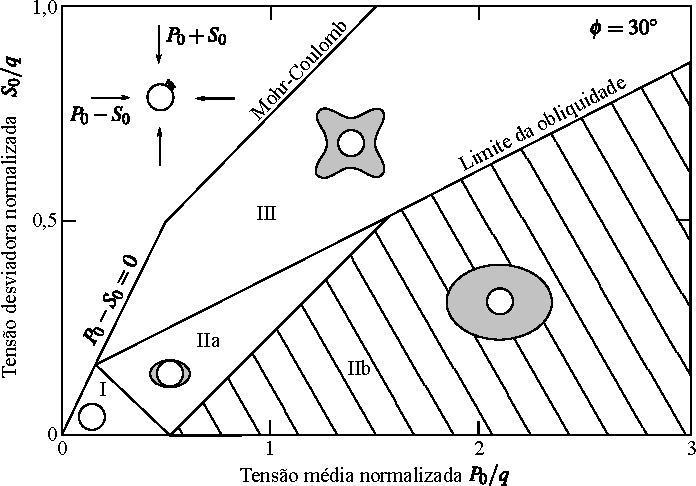
\includegraphics[scale = 1.0]{0423-modos_falha.pdf}
	\end{center}
	\caption{\label{modos_falha}Relação entre o estado de tensões iniciais e os modos de falha, onde $q$ é a resistência à compressão uniaxial do maciço (adaptado de: \citeonline[p.  121]{Detournay1988})}
\end{figure}

Como se pode ver na \autoref{modos_falha}, esses autores identificaram quatro zonas:

\begin{alineas}
	\item \textbf{região I}: a massa rochosa se comporta como um material elástico linear, ou seja, onde o estado de tensões não excedeu o critério de plasticidade em qualquer ponto;
	\item \textbf{região IIa}: a plastificação da rocha ao redor do túnel se estende em uma direção perpendicular a maior tensão principal de compressão, mas ainda não engloba completamente a seção do túnel;
	\item \textbf{região IIb}: a seção está completamente rodeada por uma zona de plastificação oval;
	\item \textbf{região III}: a zona de plastificação apresenta um formato de borboleta.
\end{alineas}

Além disso, quando há revestimento a anisotropia das tensões poderá ocasionar tração ou falha por compressão e cisalhamento na coroa ou nas paredes laterais do revestimento \cite{Brady2006}. Contudo, para uma situação em que $0 \leq K \leq 1$, em túneis profundos, a consideração de um estado geostático hidrostático ($K=1$) pode ser conservadora, para o dimensionamento do revestimento, como pode ser visto no estudo de \citeonline{Shrestha2015}.


\section{Influência da proximidade da superfície}

Quando o túnel está muito próximo da superfície, a região do maciço acima da seção não possui condições para formar a parte superior do arco transversal e desviar as tensões ao redor da cavidade. Isso faz com que essa parcela do maciço atue como sobrecarga sobre o revestimento. Dessa forma, o maciço no entorno de uma seção circular, por exemplo, não possui o campo de deslocamentos puramente radial. A rigor essa condição de túnel raso vai depender da capacidade resistente do maciço, contudo há na literatura indicações de que essa condição é atingida quando a altura de maciço sobre a coroa da seção transversal é menor que duas vezes o diâmetro \cite[p. 67]{Chapman2018}. Como consequência, a deformação da seção passa a apresentar três modos de deformações sobrepostos: uma convergência uniforme, uma distorção e translação vertical (\autoref{modos_deformacao}).

\begin{figure}[H]
	\begin{center}
		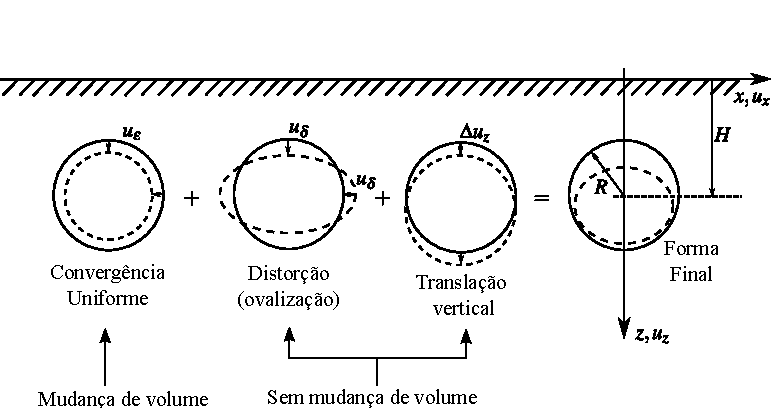
\includegraphics[scale = 1.0]{0424-modos_deformacao.pdf}
	\end{center}
	\caption{\label{modos_deformacao}Modos de deformações em túneis superficiais de seção circular (adaptado de: \citeonline[p. 4]{Pinto2014})}
\end{figure}

Quando o túnel apresenta um revestimento de concreto, por exemplo, o modo de deformação de distorção poderá induzir tensões de tração no interior do revestimento. Além disso, tão ou mais importante que a deformada da seção é o recalque induzido na superfície pelo processo de escavação. Conforme o túnel avança ele forma uma bacia de assentamento superficial que pode afetar as estruturas existentes (\autoref{bacia_assentamento}).

\begin{figure}[H]
	\begin{center}
		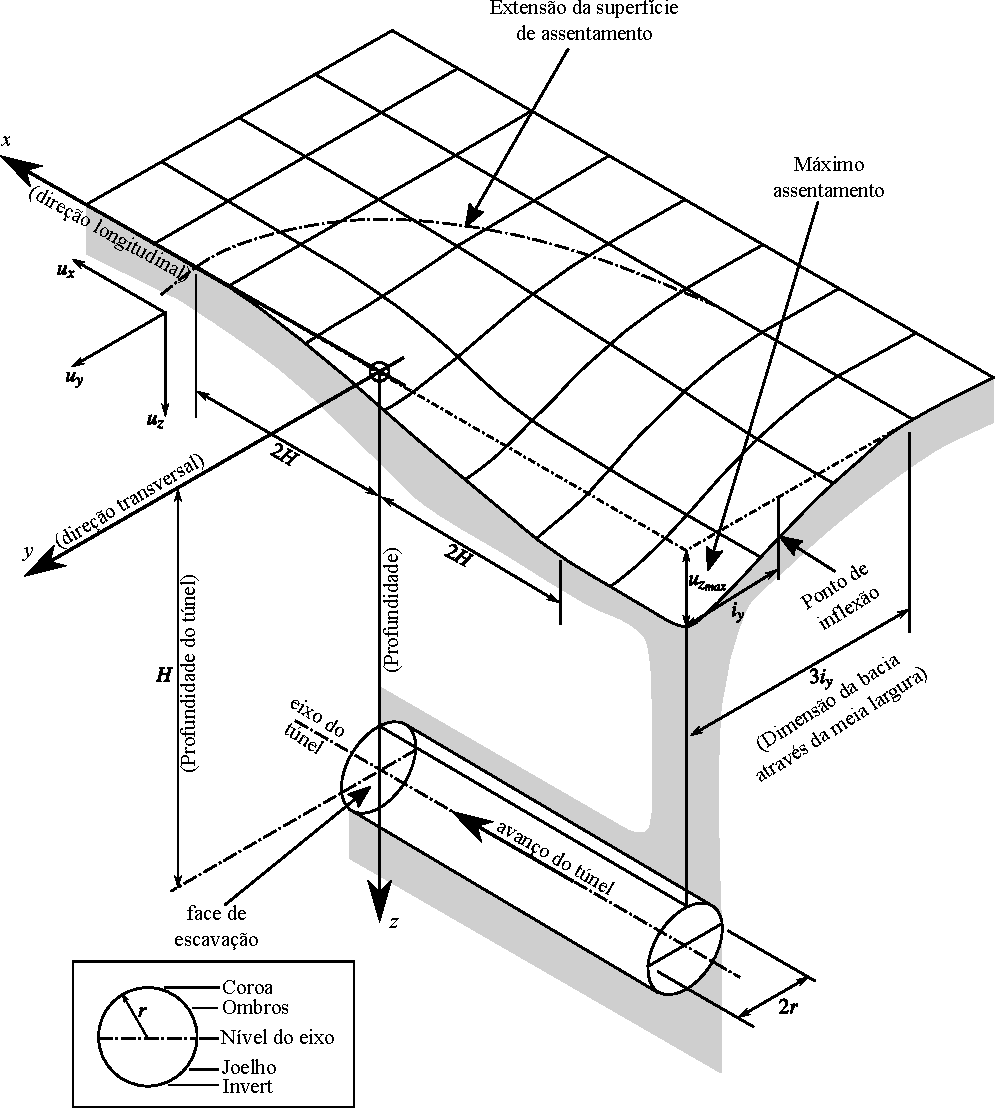
\includegraphics[scale = 1.0]{0425-bacia de assentamento.pdf}
	\end{center}
	\caption{\label{bacia_assentamento}Representação tridimensional da bacia de assentamento superficial durante a construção de um túnel superficial (adaptado de: \citeonline{Yeates1985} \textit{apud} \citeonline[p. 80]{Rankin2008})}
\end{figure}

Seguindo o trabalho de \citeonline{Martos1958} sobre assentamentos causados por minas \citeonline{Schmidt1969} e \citeonline{Peck1969}, e posteriormente muitos outros autores, mostraram que o perfil de assentamento no plano transversal pode muito bem ser descrito e ajustado, de forma empírica, através de uma curva de distribuição Gaussiana (\autoref{perfil_assentamento_transversal}).

\begin{figure}[H]
	\begin{center}
		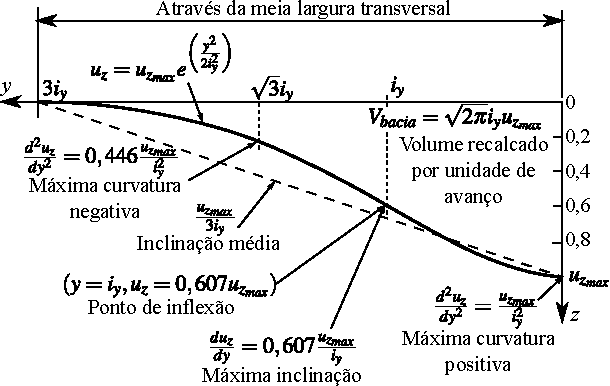
\includegraphics[scale = 1.0]{0426-perfil assentamento transversal.pdf}
	\end{center}
	\caption{\label{perfil_assentamento_transversal}Perfil idealizado de assentamento transversal com distribuição normal (adaptado de: \citeonline{OReilly1982} \textit{apud} \citeonline[p. 80]{Rankin2008})}
\end{figure}

Após \citeonline{Peck1969} propor sua forma empírica para descrever a bacia de assentamentos, adaptações dela e outros métodos semi-empíricos foram desenvolvidos com base em mais observações. Devido ao comportamento bastante específico relacionado a proximidade da superfície, os estudos sobre túneis se dividem em \textbf{túneis superficiais} e \textbf{túneis profundos}. Apesar da generalidade do modelo proposto na tese, a influência da superfície não será estudada no presente trabalho, que envolverá apenas túneis profundos, contudo, um bom resumo bibliográfico de soluções semi-empíricas pode ser encontrado em \citeonline{Zhou2018} e soluções numéricas na introdução de \citeonline{Panji2016}.

\section{Influência do revestimento e parâmetros adimensionais}

Dependendo da qualidade da rocha e das dimensões da abertura, muitos maciços conseguem desenvolver o arqueamento das tensões com pouca deformação ou ausência de plastificação. Isso caracteriza um maciço \textbf{autoportante} e, nesse caso, é necessário apenas um revestimento estético ou primário para evitar quedas localizadas. Contudo, se a redistribuição das tensões puder levar o maciço à plastificação ou deformações excessivas, nesse caso, é necessária a utilização de um \textbf{revestimento com função estrutural}. Após escavar, a redistribuição das tensões para as zonas vizinhas no interior do maciço vai depender também dos deslocamentos permitidos por esse revestimento. Dessa forma, o estado de equilíbrio após a escavação não dependerá apenas das características do maciço, tensões iniciais, da geometria da seção e escavação, mas também do comportamento conjunto do maciço com esse revestimento. Portanto, o campo de tensões e deformações dependerão da rigidez relativa entre o maciço e o revestimento, da deformação do maciço no instante de colocação do revestimento, da distância não suportada em relação à frente de escavação e, quando há comportamentos diferidos no tempo, da velocidade de avanço da construção do túnel.

A Figura 4.27 ilustra, em um corte longitudinal, o perfil de convergências e de tensões verticais sobre um túnel profundo revestido. À esquerda do ponto A o maciço encontra-se na zona não perturbada pela frente de escavação, mantendo, portanto, sua tensão vertical inicial  . Contudo, próximo à frente de escavação há um aumento das tensões verticais (entre os pontos A e B) devido ao arqueamento longitudinal das tensões próximo a face de escavação. No trecho não suportado   as tensões verticais são nulas, uma vez que não há impedimento à deformação da seção. Porém, a partir da ponta do revestimento (ponto D) há um acréscimo de tensões verticais (até o ponto E), novamente devido ao efeito de arqueamento longitudinal. Conforme a frente de escavação se afasta as tensões diminuem até atingirem um valor constante   (ponto F).

\section{Método convergência-confinamento}





% ----------------------------------------------------------
\chapter{Modelo mecânico}
\label{cap: modelo mecanico}
% ----------------------------------------------------------

Esse capítulo traz uma descrição geral do modelo mecânico que será utilizado neste trabalho. Portanto, são apresentadas as equações de equilíbrio e constitutivas que foram utilizadas, sem aprofundar, no entanto, nas particularidades que compreendem o domínio de um túnel profundo. Essas serão vistas no final do Capitulo 6, após a descrição da solução desse modelo mecânico. 

\section{Equações de Equilíbrio local e a hipótese da evolução quase estática}

Sendo $\left\{\underline{e}_1,\underline{e}_2,\underline{e}_3\right\}$ a base de um espaço $\mathbb{R}^3$, a segunda lei fundamental do equilíbrio dinâmico, ou seja, o princípio da conservação do momento linear, aplicada sobre um subdomínio contínuo $\Omega'$, exige que para $\forall \Omega' \subset \Omega$:
\begin{equation}
	\label{eq:conservacao_momento_linear}
\int_{\Omega'}\rho(\gammal-\fl)d\Omega' = \int_{\partial\Omega'}\Tl dS
\end{equation}
sendo $\rho$ a densidade do domínio, $\gammal$ o campo de acelerações referente às forças inerciais, $\fl$ o campo de acelerações referente às forças de corpo (por exemplo, a gravidade) e $\Tl$ o vetor tensão que atua na superfície $dS$ contida na superfície $\partial\Omega'$ de $\Omega'$ (\autoref{subsistema_material}).

\begin{figure}[H]
	\begin{center}
		\includegraphics[scale = 1.0]{0501-subsistema no sistema material forças de corpo.pdf}
	\end{center}
	\caption{\label{subsistema_material}Subsistema material $\Omega'$ no interior de um sistema material $\Omega$ submetido a um campo de forças de corpo}
\end{figure}

Considerando a definição $\Tl = \sigmall \cdot \nl$ , em que $\nl$ é o vetor normal à superfície $dS$ e $\sigmall$ o tensor de tensões, aplicando o teorema da divergência no termo à direita da igualdade (\ref{eq:conservacao_momento_linear}) pode-se escrever que
\begin{equation}
	\label{teorema_divergencia}
	\forall \Omega' \subset \Omega ~~~~ \int_{\Omega'}\left( \divl \sigmall+ \rho(\gammal-\fl) \right)d\Omega' = \underline 0
\end{equation}
e, portanto,
\begin{equation}
	\label{eq:resultado_teorema_divergencia}
	 \underline \nabla \cdot \underline{\underline\sigma}+ \rho(\underline\gamma-\underline f) = \underline 0
\end{equation}
em que $\divl$ é o operador divergente. Aplicando a hipótese de evolução quase estática, ou seja, $\gammal = \underline 0$, tem-se o seguinte sistema de equações de equilíbrio estático local:
\begin{equation}
	\label{eq:equilibrio_estatico_local}
	\divl \sigmall+ \rho \fl = \underline 0.
\end{equation}

Salienta-se também que pela conservação do momento angular tem-se que o tensor de tensões é simétrico, ou seja, $\sigmall = \sigmall^T$ e o sistema (\ref{eq:equilibrio_estatico_local}), em três dimensões, possui 3 equações e 6 incógnitas de tensões.

\section{Admissibilidade estática, natureza Euleriana do Campo de Tensões, Transformação geométrica e medida de deformação}

Para que o sistema material $\Omega$ da \autoref{sistema_material_contorno} esteja em equilíbrio, ou seja, \textbf{estáticamente admissível (E.A)}, o campo de tensões deve satisfazer as equações de campo de equilíbrio local, conjuntamente com as condições de continuidade interna e de contorno (relativo ao princípio da ação-reação) representadas por (\ref{eq:EA}).

\begin{figure}[H]
	\begin{center}
		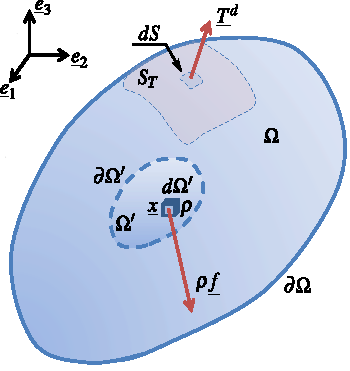
\includegraphics[scale = 1.0]{0502-sistema material com condição de contorno.pdf}
	\end{center}
	\caption{\label{sistema_material_contorno}Sistema material $\Omega'$ com condição de contorno $\underline T^d$ imposta na fronteira $S_T$}
\end{figure}

\begin{equation}
	\label{eq:EA}
	\sigmall~~ \text{é E.A.} \leftrightarrow \left\{
		\begin{matrix}
			\text{eqs. campo:} \left\{
				\begin{matrix}
					\divl \sigmall+ \rho \fl = \underline 0 \\ 
					\sigmall \cdot \nl ~~ \text{contínuo ao longo de} ~~ \Sigma
		
				\end{matrix}\right. \\ 
			\text{cond. contorno:}~~ \sigmall \cdot \nl = \Tl^d ~~ \text{em} ~~ \forall \xl \in S_T \subset \partial \Omega
		\end{matrix}\right.,
\end{equation}

em que $\Sigma$  representa as superfícies de descontinuidades de $\sigmall$ no interior do corpo, se houver. A rigor o campo de tensões $\sigmall$ que satisfaz (\ref{eq:EA}) se refere sempre à configuração atual durante a evolução do sistema, ou seja, possui uma natureza Euleriana (conforme \autoref{tensoes_Euleriana}).

\begin{figure}[H]
	\begin{center}
		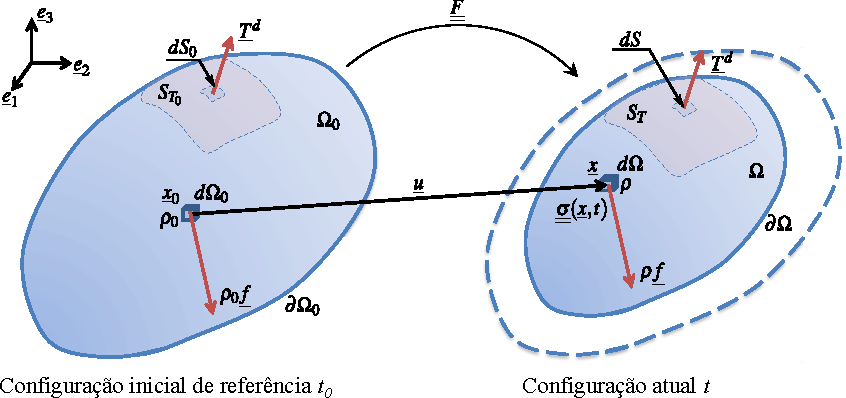
\includegraphics[scale = 1.0]{0503-descricao euleriana do campo de tensoes.pdf}
	\end{center}
	\caption{\label{tensoes_Euleriana}Natureza Euleriana do campo de tensões}
\end{figure}

O vetor $\ul = \xl - \xl_0$ é o deslocamento da partícula durante a evolução do sistema e $\Fll$ é o gradiente da transformação geométrica que associa a posição de cada partícula $\xl_0$ a sua posição $\xl$ na configuração atual, definido por:
\begin{equation}
	\label{eq:transformacao_geometrica}
 	\Fll = \nabla \xl = \nabla \left( \xl_0+\ul \right) = \Umll + \nabla \ul
\end{equation}
em que $\nabla$ é o operador gradiente e $\Umll$ o tensor de segunda ordem unitário. Nesse contexto geral, a medida de deformação mais comum é dada pelo desvio da transformação em relação à isometria $\Fll^T \cdot \Fll = \Umll$ e é descrita através do tensor de deformações de Green-Lagrange:
\begin{equation}
	\label{eq:green_lagrange}
	\greenll = \frac{1}{2} \left(\Fll^T \cdot \Fll - \Umll \right) = \frac{1}{2} \left(\nabla \ul + \nabla\ul^T + \nabla\ul^T \cdot \nabla \ul \right).
\end{equation}

Em problemas quase-estáticos isotérmicos, quando os deslocamentos, as deformações e as rotações são pequenas, a determinação dos campos de tensões e deformações durante a evolução do sistema pode ser simplificada descrevendo os elementos da admissibilidade estática (\ref{eq:EA}) em termos da configuração de referência ao invés da atual. Para tanto, é necessário verificar-se a hipótese das pequenas perturbações.

\section{Hipótese das pequenas perturbações e a descrição Lagrangeana}

A \textbf{hipótese das transformações infinitesimais (HTI)} supõe que o gradiente da transformação é aproximadamente a identidade, ou seja, $\Fll \approx \Umll$ . Isso implica, por (\ref{eq:transformacao_geometrica}), que $\left| \nabla \ul \right| \ll 1$ e, como consequência, pode-se desprezar os termos de derivada mais alta no tensor de deformações de Green-Lagrange, de modo que:
\begin{equation}
	\label{eq:green_lagrange_linearizado}
	\greenll = \frac{1}{2} \left(\Fll^T \cdot \Fll - \Umll \right) = \frac{1}{2} \left(\nabla \ul + \nabla\ul^T + \nabla\ul^T \cdot \nabla \ul \right) \approxeq \frac{1}{2} \left(\nabla \ul + \nabla\ul^T \right) = \nabla^s\ul = \varepsilonll
\end{equation}
em que $\varepsilonll$ é um tensor simétrico conhecido como tensor de deformações de Green-Lagrange linearizado, ou simplesmente, como tensor de deformações. Dessa hipótese segue-se também uma simplificação no \textbf{Jacobiano da transformação} (que dá a relação entre o volume infinitesimal da configuração atual e de referência):
\begin{equation}
	\label{eq:jacobiano}
	J = \frac{d\Omega}{d\Omega_0} = \text{det}\left(\Umll + \nabla \ul \right) \approxeq 1 + \text{tr}(\varepsilonll)
\end{equation}
sendo det($*$) e tr($*$) as funções determinante e traço, respectivamente. Como  $\left| \nabla \ul \right| \ll 1$ tem-se também que $\left| \nabla \varepsilonll \right| \ll 1$, ou seja, \textbf{pequenas deformações}, o que implica $\text{tr}(\varepsilonll) \ll 1$ e, portanto, mudanças infinitesimais no volume e na densidade durante a evolução do sistema, fazendo com que $\Omega \approxeq \Omega_0$ e $\rho \approxeq \rho_0$, respectivamente. Supondo que também ocorram \textbf{pequenos deslocamentos} $\left| \ul / l_0 \right| \ll 1$, em que $l_0$ é uma dimensão característica do problema tal que os efeitos sobre os esforços internos devido a mudança de geometria sejam desprezíveis, tem-se a \textbf{hipótese das pequenas perturbações (HPP)}. Com as consequências dessa hipótese, pode-se adotar a configuração inicial (de referência) ao invés da atual para expressar os termos da admissibilidade estática  (\ref{eq:EA}).

\section{Modelo constitutivo elástico}

De uma forma geral, a energia interna específica $w$  necessária para deformar um material elástico não depende do trajeto e nem da velocidade de deformação durante a evolução do sistema, dependendo apenas do estado atual das deformações. Com isso a energia interna específica pode ser caracterizada pelas deformações e direções principais do tensor de deformações, de modo que:
\begin{equation}
	\label{eq:energia_interna_elastica}
	w(\varepsilonll) = w(\varepsilon_1,\varepsilon_2,\varepsilon_3,\eta_1,\eta_2,\eta_3).
\end{equation}

Contudo, na \textbf{elasticidade isótropa} a energia de deformação é independente das direções principais e pode ser descrita em função apenas da magnitude das deformações principais, ou dos invariantes do tensor de deformação, de modo que
\begin{equation}
	\label{eq:energia_interna_elastica_isotropa}
	w(\varepsilonll) = w(\varepsilon_1,\varepsilon_2,\varepsilon_3) = w(I_1,I_2,I_3),
\end{equation}
sendo que os invariantes do tensor de deformações são dados por:
\begin{equation}
	\label{eq:I1}
	I_1 = \text{tr}(\varepsilonll) = \varepsilon_{ii},
\end{equation}
\begin{equation}
	\label{eq:I2}
	I_2 = \text{tr}(\varepsilonll^2) = \frac{1}{2} \varepsilon_{ij} \varepsilon_{ji},
\end{equation}
\begin{equation}
	\label{eq:I3}
	I_3 = \text{tr}(\varepsilonll^3) = \frac{1}{3} \varepsilon_{ij} \varepsilon_{jk} \varepsilon_{ki}.
\end{equation}

A lei do comportamento elástico se obtém de $\sigmall = \partial w / \partial \varepsilonll$ . Aplicando a regra da cadeia em relação aos invariantes e fazendo uma aproximação de primeira ordem em torno de $\sigmall_0$ tem-se a seguinte lei constitutiva da \textbf{elasticidade linear isótropa}
\begin{equation}
	\label{eq:lei_elasticidade}
	\sigmall - \sigmall_0 = \Dllll:\varepsilonll,
\end{equation}
em que $\Dllll$ é o tensor constitutivo elástico de quarta ordem simétrico dado por
\begin{equation}
	\label{eq:tensor_constitutivo_elastico}
 	\Dllll = \lambda^e \Umll \otimes \Umll + 2 \mu^e \Umllll
\end{equation}
sendo $\underline{\underline 1} \otimes \underline{\underline 1}$ o tensor de quarta ordem dado pelo produto tensorial ($\otimes$) entre dois tensores unitários de segunda ordem e $\underline{\underline{\underline{\underline 1}}}$ o tensor unitário de quarta ordem. As constantes $\lambda^e$ e $\mu^e$ são conhecidos como os coeficientes de Lamè, que possuem as seguintes relações com o módulo de Young $E$ e o coeficiente de Poisson $\nu$:
\begin{equation}
	\label{eq:lambdae}
	\lambda^e = \frac{E \nu}{(1+\nu)(1-2\nu)},
\end{equation}
\begin{equation}
	\label{eq:mue}
	\mu^e = \frac{E}{2(1+\nu)}.
\end{equation}

\section{Modelo constitutivo elastoplástico}

Para problemas com evolução isotérmica, quase-estáticos em transformações infinitesimais, o modelo constitutivo elastoplástico pode ser completamente descrito através da:
\begin{alineas}
	\item decomposição do tensor de deformação total;
	\item superfície de escoamento;
	\item regra de fluxo plástico;
	\item lei de endurecimento/amolecimento;
	\item condições de carregamento/descarregamento.
\end{alineas}

\subsection{Decomposição do tensor de deformação total}
Considerando a hipótese das pequenas transformações (que inclui a hipótese das pequenas deformações) é válida a decomposição do tensor de deformação total em uma componente elástica e outra plástica, de modo que:
\begin{equation}
	\label{eq:decomposicao_deformacoes}
	\dot \varepsilonll = \dot \varepsilonll^e + \dot \varepsilonll^p 
\end{equation}
sendo $\dot \varepsilonll^e$ e $\dot \varepsilonll^p$ as taxas de deformação elástica e plástica, respectivamente. A taxa de deformação plástica também é conhecida por fluxo plástico. Diferentemente do modelo elástico, o modelo elastoplástico é dependente do trajeto das tensões e por isso (\ref{eq:decomposicao_deformacoes}) é descrito em forma de taxas. No entanto, na elastoplasticidade, o tempo físico não entra nas leis constitutivas, tratando-se de um fenômeno instantâneo. A marcação do tempo serve apenas para acompanhar o histórico de tensões, se tratando, portanto, de um pseudo-tempo.

Dentro do contexto de processos termodinâmicos determinísticos, a energia livre específica $\psi$ de um material elastoplástico do qual se deriva as relações constitutivas, para o caso de uma evolução isotérmica em pequenas deformações, pode ser escrita e decomposta da seguinte maneira \cite[p. 149]{Neto2008}:
\begin{equation}
	\label{eq:energia_livre}
	\psi(\varepsilonll,\varepsilonll^p,\alphal) = \psi^e(\varepsilonll-\varepsilonll^p)+ \psi^p(\alphal) = \psi^e(\varepsilonll^e)+ \psi^p(\alphal) 
\end{equation}
em que $\alphal$ é o conjunto de variáveis internas (coesão, ângulo de atrito e etc) cuja evolução está relacionada com o fenômeno de endurecimento/amolecimento. Dessa expressão e da aplicação da segunda lei da termodinâmica, que leva à inequação de Clausius-Duhem, deriva-se as seguintes relações constitutivas:
\begin{equation}
	\label{eq:leielastoplasticidade}
		\left\{
		\begin{array}{rcl}
			\sigmall = \dfrac{\partial \psi^e}{\partial \varepsilonll^e} \\ 
			\ql = \dfrac{\partial \psi^p}{\partial \alphal}
			
		\end{array}
		\right.
\end{equation}
em que $\ql$ é o conjunto das forças termodinâmicas (escalares ou tensoriais) associadas às variáveis internas. De (\ref{eq:decomposicao_deformacoes}) e (\ref{eq:leielastoplasticidade})$_1$ obtem-se a seguinte relação constitutiva:
\begin{equation}
	\label{eq:leielastoplastica}
	\dot \sigmall = \Dllll^{ep}:\dot \varepsilonll = \Dllll:\dot \varepsilonll^e = \Dllll:\left(\dot \varepsilonll - \dot \varepsilonll^p \right)
\end{equation}
em que $\Dllll^{ep}$ é um tensor de quarta ordem que representa o módulo elastoplástico contínuo.

\subsection{Superfície de escoamento}
Uma característica fenomenológica dos materiais elastoplásticos é a existência de um limite dentro do qual o material se comporta elasticamente. Em problemas tridimensionais isotrópicos esse domínio é delimitado por uma hiper superfície no espaço das tensões principais, chamada de \textbf{superfície de escoamento}, pois, assim que o estado de tensões atinge essa superfície tem inicio a evolução das deformações plásticas. Essa superfície é definida como \cite[p. 150]{Neto2008}:
\begin{equation}
	\label{eq:superficie_escoamento}
	\partial \Gamma = \left\{ \sigmall | f(\sigmall,\ql) = 0 \right\}
\end{equation}
em que $f$ é a \textbf{função de escoamento}. Essa superfície delimita o conjunto de tensões que estão dentro do domínio elástico, ou seja, \textbf{elasticamente admissíveis (E. A.)}:
\begin{equation}
	\label{eq:dominio_elasticamente_admissivel}
	\Gamma^* = \left\{ \sigmall | f(\sigmall,\ql) < 0 \right\},
\end{equation}
e o conjunto de tensões \textbf{plasticamente admissíveis (P. A.)}:
\begin{equation}
	\label{eq:dominio_plasticamente_admissivel}
	\Gamma = \left\{ \sigmall | f(\sigmall,\ql) \le 0 \right\}.
\end{equation}

A \autoref{dominio_plasticamente_admissivel} ilustra de uma forma genérica esse domínio plasticamente admissível no espaço das tensões principais.
\begin{figure}[H]
	\begin{center}
		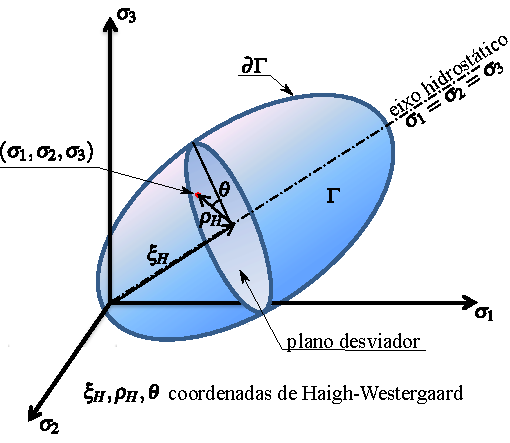
\includegraphics[scale = 1.0]{0504-dominio generico plasticamente admissivel.pdf}
	\end{center}
	\caption{\label{dominio_plasticamente_admissivel}Domínio genérico plasticamente admissível $\Gamma$ no espaço das tensões principais}
\end{figure}
Em elastoplasticidade isotrópica, a função de escoamento pode ser descrita apenas em função dos invariantes do tensor de tensões e das forças associadas às variáveis internas. São, portanto, comuns as seguintes representações equivalentes (adaptado de \citeauthor{Chen1988}, \citeyear{Chen1988}, p. 57-72):
\begin{equation}
	\label{eq:funcoes_escoamento}
	f(\sigmall,\ql) = f(I_1,J_2,J_3,\ql) = f(\xi_{H},\rho_{H},\theta,\ql) = f(p,q,\theta,\ql) = f(\sigma_{oct},\tau_{oct},\theta,\ql)
\end{equation}
em que:
\begin{equation}
	\label{eq:invariantes_tensores}
		\begin{array}{lcl}
			I_1 = \text{tr}(\sigmall) = \sigma_{11}+\sigma_{22}+\sigma_{33}\\
			J_2 = \dfrac{1}{2}\text{tr}(\sll^2) = \dfrac{1}{6}\left[ (\sigma_{11}-\sigma_{22})^2 + (\sigma_{22}-\sigma_{33})^2 + (\sigma_{33}-\sigma_{11})^2 \right] + \sigma_{12}^2+ \sigma_{23}^2+ \sigma_{13}^2, \\
			J_3 = \dfrac{1}{3}\text{tr}(\sll^3) = \text{det}(\sll) = s_{11}s_{22}s_{33}-s_{11}\sigma_{23}^2-s_{22}\sigma_{13}^2-s_{33}\sigma_{12}^2+2\sigma_{12}\sigma_{23}\sigma_{13}, \\ 
			\xi_{H} = p = \sigma_{oct} = \dfrac{1}{3}I_1, ~~~ \rho_{H} = \sqrt{\sll:\sll} = \sqrt{2J_2}, ~~~ \theta = \dfrac{1}{3}arcsen\left( \dfrac{-3\sqrt{3}}{2} \dfrac{J_3}{J_2^{3/2}} \right), \\
			-\dfrac{\pi}{6} \le \theta \le \dfrac{\pi}{6}, ~~~ q = \sqrt{\dfrac{3}{2}\sll:\sll} = \sqrt{3J_2}, ~~~ \tau_{oct} = \sqrt{\dfrac{3}{2}J_2},
	\end{array}
\end{equation}
sendo $(\xi_H,\rho_H,\theta)$ as coordenadas de Haigh-Westergaard (em que $\theta$ também é conhecido como ângulo de Lode), $p$ a pressão hidrostática, $q$ a tensão equivalente de von-Mises, $(\sigma_{oct},\tau_{oct})$ a tensão normal e cisalhante octaédrica, respectivamente, e $s_{ij}$ são as componentes do tensor de tensões desviadoras $\sll$, dado por:
\begin{equation}
	\label{eq:tensor_desviador}
	\sll = \sigmall: \left[ \Umllll-\Umll \otimes \Umll \right] = \sigmall - p\Umll.
\end{equation}

Quando a função de escoamento não depende de $I_1$   diz-se que a plasticidade é independente da pressão hidrostática, sendo determinada apenas pelo estado de tensões ao longo do plano desviador.

Diversas funções de escoamentos podem ser obtidas na literatura, tal como as apresentadas no resumo de \citeonline{Viladkar1995} que reúne tanto as funções de escoamentos clássicas (von-Mises, Tresca, Drucker-Prager, Mohr-Coulomb) quanto mais sofisticadas (\textit{Cap Models, Critical State Model, Desai’s Generlized Model}). O presente trabalho utilizará as funções de escoamentos de Drucker-Prager e Mohr-Coulomb que compreendem também generalizações das funções de von-Mises e Tresca, respectivamente (\autoref{Funções_escoamento}).
\begin{figure}[H]
	\begin{center}
		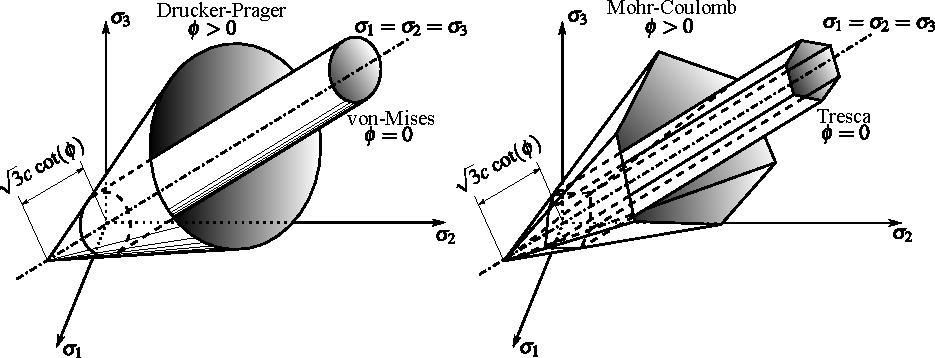
\includegraphics[scale = 1.0]{0505-funções de escoamento.pdf}
	\end{center}
	\caption{\label{Funções_escoamento}Funções de escoamento de a) Drucker-Prager e b) Mohr-Coulomb  (adaptado de: \citeonline[p. 824]{Zienkiewicz1974})}
\end{figure}
A função de escoamento de Mohr-Coulomb, representada através de invariantes, é dada por \cite[p. 166]{Neto2008}:
\begin{equation}
	\label{eq:f_Mohr_Coulomb}
	f(\sigmall,\ql) = f(I_1,J_2,\theta,c,\phi) = \dfrac{\sin(\phi)}{3}I_1 + \left(\cos(\theta)-\dfrac{1}{\sqrt{3}}\sin(\theta)\sin(\phi)\right)\sqrt{J_2}-c\cos(\phi) 
\end{equation}
em que $c$ é a coesão e $\phi$ o ângulo de atrito. De forma análoga, a função de escoamento de Drucker-Prager é dada por \cite[p. 167]{Neto2008}:
\begin{equation}
	\label{eq:f_Drucker_Prager}
	f(\sigmall,\ql) = f(I_1,J_2,\beta,k) = \beta I_1 +\sqrt{J_2}-k
\end{equation}
em que os parâmetros $\beta$ e $k$ podem ser relacionados com a coesão e o ângulo de atrito do modelo de Mohr-Coulomb. Para o caso em que a superfície de Drucker-Prager coincide com as bordas mais externas da superfície de Mohr-Coulomb tem-se \cite[p. 167]{Neto2008}:
\begin{equation}
	\label{eq:f_DP_bordasexternas_MC}
	\beta = \dfrac{2\sin{\phi}}{\sqrt{3}(3-\sin(\phi))}, ~~~ k = \dfrac{6\cos{\phi}}{\sqrt{3}(3-\sin(\phi))}c,
\end{equation}
e para o caso em que a superfície de Drucker-Prager coincide com as bordas mais internas da superfície de Mohr-Coulomb, tem-se \cite[p. 167]{Neto2008}:
\begin{equation}
	\label{eq:f_DP_bordasinternas_MC}
	\beta = \dfrac{2\sin{\phi}}{\sqrt{3}(3+\sin(\phi))}, ~~~ k = \dfrac{6\cos{\phi}}{\sqrt{3}(3+\sin(\phi))}c.
\end{equation}

Essa aproximação pode ser vista no plano desviador conforme a \autoref{DP-MC-plano_desviador}.
\begin{figure}[H]
	\begin{center}
		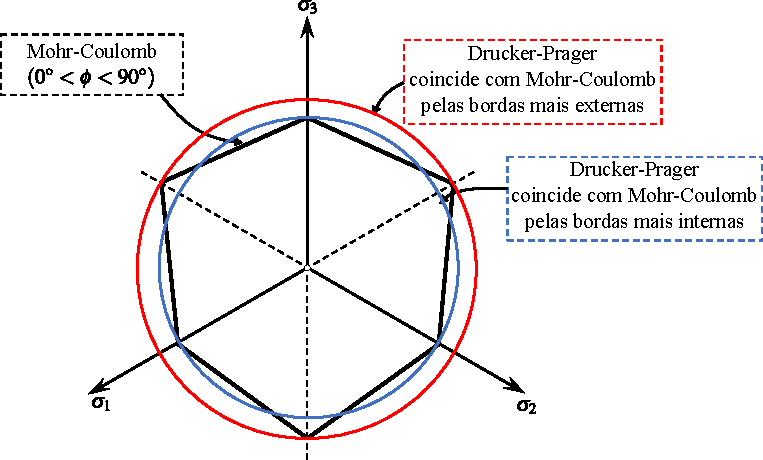
\includegraphics[scale = 1.0]{0506-representação no plano desviador da aproximação da superficie de MC com DP.pdf}
	\end{center}
	\caption{\label{DP-MC-plano_desviador}Representação no plano desviador da aproximação da superfície de Mohr-Coulomb pela superfície de Drucker-Prager  (adaptado de: \citeauthor{Neto2008}, \citeyear{Neto2008}, p. 169)}
\end{figure}
Quando $\phi = 0$ a superfície de Mohr-Coulomb e a de Drucker-Prager se tornam independentes da pressão hidrostática e se particularizam, respectivamente, para a superfície de Tresca e von-Mises:
\begin{equation}
	\label{eq:f_Tresca}
	f(\sigmall,\ql) = f(J_2,\theta,c) = \sqrt{J_2}\cos{\theta} - c,
\end{equation}
\begin{equation}
	\label{eq:f_von-Mises}
	f(\sigmall,\ql) = f(J_2,\theta,c) = \sqrt{J_2} - \dfrac{2c}{\sqrt{3}}.
\end{equation}

Igualando-se as expressões (\ref{eq:f_von-Mises}) e (\ref{eq:f_Tresca}) à zero e isolando $\sqrt{J_2}$ é possível relacionar ambas as superfícies através da coesão (\autoref{TR-VM-plano_desviador}):
\begin{equation}
	\label{eq:ctr_cvm}
	c_{TR} = \dfrac{2}{\sqrt{3}}\cos(\theta)c_{VM} = \left\{
	\begin{array}{lcl}
		\dfrac{2}{\sqrt{3}}c_{VM}, ~~~\text{se}~\theta = 0^\circ \\ 
		c_{VM},~~~~~~~~~\text{se}~\theta = 30^\circ
	\end{array}
	\right..
\end{equation}
\begin{figure}[H]
	\begin{center}
		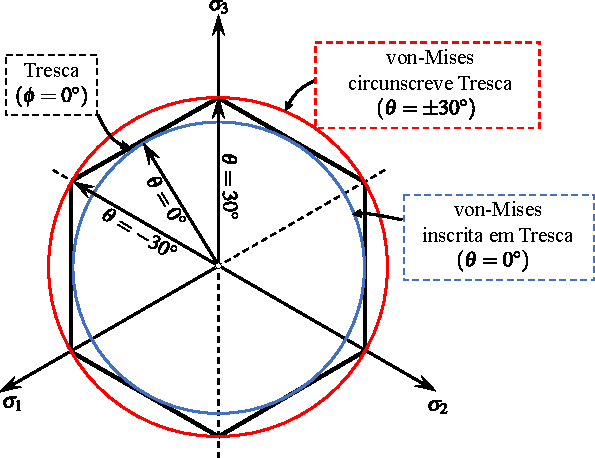
\includegraphics[scale = 1.0]{0507-representação no plano desviador da aproximação da superfície de TR e VM.pdf}
	\end{center}
	\caption{\label{TR-VM-plano_desviador}Representação no plano desviador da aproximação da superfície de Tresca pela superfície de von-Mises (adaptado de: \citeauthor{Neto2008}, \citeyear{Neto2008}, p. 159, 164)}
\end{figure}

\subsection{Regra de fluxo plástico}

A regra de fluxo plástico descreve a lei de evolução das deformações plásticas com relação às tensões. Essa regra é postulada da seguinte forma:
\begin{equation}
	\label{eq:fluxo_elastoplastico}
	\dot \varepsilonll^p = \dot \lambda \dgdsll
\end{equation}
em que $\dot \lambda$ é a taxa da magnitude de deformação plástica $\lambda$ (chamado também de multiplicador plástico) e $\dgdsll$ o tensor que dá a direção do fluxo plástico (conhecido também como vetor de fluxo ou gradiente do potencial plástico), sendo definido como:
\begin{equation}
	\label{eq:vetor_fluxo_elastoplastico}
	\dgdsll = \dfrac{\partial g}{\partial \sigmall}
\end{equation}
em que $g$ é uma função análoga a $f$ chamada de potencial plástico. No caso em que $g=f$ tem-se a \textbf{plasticidade associada} (ou seja, a direção do fluxo plástico é perpendicular à superfície de plastificação) (\autoref{fluxo_associado}).
\begin{figure}[H]
	\begin{center}
		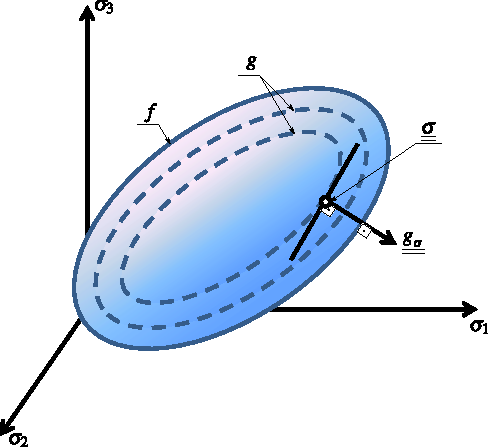
\includegraphics[scale = 1.0]{0508-representacao geometrica do vetor de fluxo com plasticidade associada.pdf}
	\end{center}
	\caption{\label{fluxo_associado}Representação geométrica do vetor de fluxo em plasticidade associada (adaptado de: \citeonline[p. 182]{Chen1988})}
\end{figure}
Tal como a função de escoamento, o potencial plástico geralmente é descrito através dos invariantes do tensor de tensões e seu gradiente pode ser determinado aplicando a regra da cadeia em (\ref{eq:vetor_fluxo_elastoplastico}). Por exemplo, se $g(I_1,\sqrt{J_2},J_3,\ql)$, tem-se (adaptado de \citeauthor{Viladkar1995}, \citeyear{Viladkar1995}, p. 333):
\begin{equation}
	\label{eq:invariantes_tensores}
	\begin{array}{lcl}
		\dgdsll = C_1\gllum + C_2\glldois + C_3\glltres, \\ 
		\gllum = \dfrac{\partial I_1}{\partial \sigmall} = \Umll,~~~ \glldois = \dfrac{\partial \sqrt{J_2}}{\partial \sigmall} = \dfrac{1}{2\sqrt{J_2}}\sll,~~~ \glltres = \dfrac{\partial J_3}{\partial \sigmall}, \\
		C_1 = \dfrac{\partial g}{\partial I_1},~~~C_2=\dfrac{\partial g}{\partial \sqrt{J_2}}-\dfrac{\tan{(3\theta)}}{\sqrt{J_2}}\dfrac{\partial g}{\partial \theta},~~~C_3 = \dfrac{\sqrt{3}}{2\cos{(3\theta})}-\dfrac{1}{J_2^{3/2}}\dfrac{\partial g}{\partial \theta},
	\end{array}
\end{equation}
sendo que nessa descrição, apenas as constantes $C_1$, $C_2$  e $C_3$ são particularidades das diferentes superfícies potenciais. Para a superfície de Mohr-Coulomb tem-se:
\begin{equation}
	\label{eq:c1MC}
	C_1 = \dfrac{1}{3}\sin(\phi),
\end{equation}
\begin{equation}
	\label{eq:c2MC}
	C_2 = \cos(\theta)\left[1+\tan(\theta)\tan(3\theta) + \dfrac{\sin(\phi)\left(\tan(3\theta)-\tan(\theta)\right)}{\sqrt{3}}\right],
\end{equation}
\begin{equation}
	\label{eq:c3MC}
	C_3 = \dfrac{\sqrt{3}\sin(\theta)+\cos(\theta)\sin(\phi)}{2J_2\cos(3\theta)},
\end{equation}
e para Drucker-Prager, tem-se:
\begin{equation}
	\label{eq:c1c2c3DP}
	C_1 = \beta,~~~C_2 = 1,~~~C_3 = 0.
\end{equation}

Nas expressões de $C_2$ e $C_3$, pode-se ver que o vetor de fluxo de Mohr-Coulomb, e consequentemente o de Tresca, possui uma singularidade quando $\theta = \pm \pi/6$. Isso ocorre devido a essas superfícies apresentarem um vértice nessas coordenadas no plano desviador. Há diversas formas de se resolver esse problema, sendo que a adotada no presente trabalho, dada por \citeonline[p. 234]{Owen1980}, será utilizar os valores de $C_1$,$C_2$ e $C_3$ de Drucker-Prager (ou von-Mises) quando $\theta = \pm \pi/6$.

Um aspecto comum na geomecânica é a variação do volume do material durante a evolução das deformações plásticas. Esse efeito é comumente introduzido através da plasticidade não associada, adotando, ao invés do ângulo de atrito, um ângulo de dilatância $0<\psi<\phi$  na função potencial $g$.

\subsection{Lei de endurecimento/amolecimento}
A lei de endurecimento/amolecimento caracteriza, em geral, a dependência das variáveis internas (por exemplo, a coesão e o ângulo de atrito) em relação ao histórico de deformações plásticas. Essa lei de endurecimento/amolecimento é postulada da seguinte forma \cite[p. 249]{Belytschko2000}:
\begin{equation}
	\label{eq:amolecimento}
	\dot \ql = \dot \lambda \hl(\sigmall,\ql)
\end{equation}
em que $\hl$ é um vetor que contém os gradientes de uma função potencial $h$ com relação à cada força associada a sua respectiva variável interna. Como a função de escoamento $f$ é dependente das forças termodinâmicas associadas ao conjunto de variáveis internas $\alphal$, a mudança dessas ao longo da deformação plástica irá alterar a posição e/ou a forma da superfície de escoamento. Quando a superfície de escoamento é estática, ou seja, $\dot \ql=\underline 0$, tem-se a plasticidade perfeita, quando esta aumenta tem-se o endurecimento isotrópico e quando se desloca tem-se o endurecimento cinemático (\autoref{tipos_endurecimento}), sendo mista, quando composta das duas últimas.

\begin{figure}[H]
	\begin{center}
		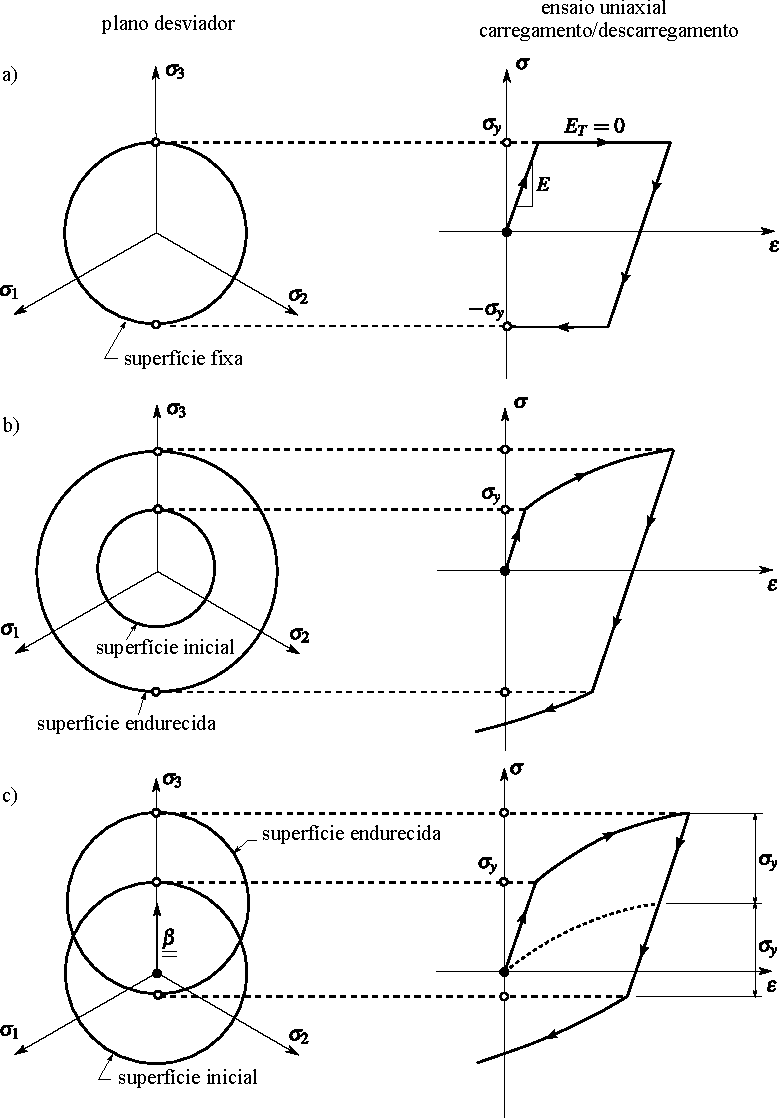
\includegraphics[scale = 1.0]{0509-tipos_endurecimentos.pdf}
	\end{center}
	\caption{\label{tipos_endurecimento}Representação dos tipos de endurecimento no plano desviador e na curva tensão-deformação: a) elastoplasticidade perfeita, b) endurecimento isotrópico e c) endurecimento cinemático (adaptado de: \citeauthor{Neto2008}, \citeyear{Neto2008}, p. 178, 179, 186)}
\end{figure}

Em um primeiro momento, no presente trabalho, não será considerado a influência da lei de endurecimento e, portanto, as variáveis internas serão constantes ao longo do histórico de deformações, ou seja, $\dot \ql = \dot \alphal = \underline 0$. Nesse caso, tem-se a elastoplasticidade perfeita. Para os modelos adotados significa que a coesão e o ângulo de atrito permanecem constantes durante a deformação plástica. Em um segundo momento é implementado uma função linear definida por partes para representar o endurecimento/amolecimento característico do maciço, tal como vistos no Capítulo 4.3, contudo em caráter associado ($h = f$) e isotrópico. Essa implementação, é feita exclusivamente através da coesão que dependerá da magnitude das deformações plásticas ao longo do histórico de tensões (conforme \autoref{funcao_coesao}).

\begin{figure}[H]
	\begin{center}
		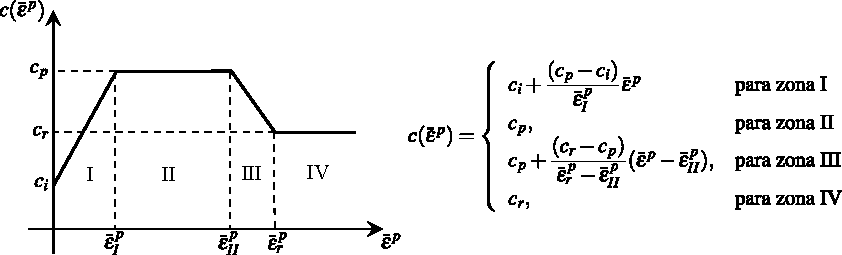
\includegraphics[scale = 1.0]{0510-lei de endurecimento ou amolecimento_coesao.pdf}
	\end{center}
	\caption{\label{funcao_coesao}Função linear definida por partes para representar o endurecimento/amolecimento através do parâmetro coesivo (adaptado de: \citeonline[p. 158]{Potts1999}}
\end{figure}
Portanto, usando a regra da cadeia, escreve-se (\ref{eq:amolecimento}) da seguinte forma: 
\begin{equation}
	\label{eq:expressao_amolecimento}
	\dot \ql = \left\{ \begin{array}{l} \dot c \\ \dot \phi \end{array} \right\} = \dot \lambda \left\{ \begin{array}{ccc} \dfrac{\partial f}{\partial c}\dfrac{\partial c}{\partial \bar \epsilon^p} \\ 0 \end{array} \right\}.
\end{equation}
em que, conforme (\ref{eq:f_Mohr_Coulomb}) e (\ref{eq:f_Drucker_Prager}), tem-se:
\begin{equation}
	\label{eq:dfdc}
	\dfrac{\partial f}{\partial c} = \left\{ \begin{array}{ll} - \cos(\phi), & \text{para Mohr-Coulomb} \\ - \dfrac{6\cos(\phi)}{\sqrt{3}(3\pm \sin(\phi))}, & \text{para Drucker-Prager}\end{array}\right.
\end{equation}
e
\begin{equation}
	\label{eq:dcde}
	\dfrac{\partial c}{\partial \bar \epsilon_{p}} = \left\{ \begin{array}{ll} \dfrac{(c_p-c_i)}{\bar \epsilon^p_I} &  \text{para zona I} \\ 
	c_p, & \text{para zona II} \\
	\dfrac{(c_r-c_p)}{\bar \epsilon^p_{r}-\bar \epsilon^p_{II}}, & \text{para zona III} \\	
	c_r, & \text{para zona IV}
\end{array}\right..
\end{equation}


\subsection{Condições de carregamento e descarregamento}

A evolução das equações (\ref{eq:fluxo_elastoplastico}) e (\ref{eq:amolecimento}) estão sujeitas à três condições (condições de Kuhn-Tucker), que são (\citeauthor{Neto2008}, \citeyear{Neto2008}, p. 170):
\begin{equation}
	\label{eq:kuhntucker}
	f \le 0,~~~ \dot \lambda \ge 0, ~~~ \dot \lambda f = 0.
\end{equation}
Essas condições estabelecem que apenas ocorre fluxo plástico quando o estado de tensões está sobre a superfície de escoamento e, neste caso, não há variação da função de escoamento, ou seja:
\begin{equation}
	\label{eq:consistencia}
	\dot f = \dfrac{\partial f}{\partial \sigmall}:\dot \sigmall + \dfrac{\partial f}{\partial \ql}\cdot \dot \ql = \dfdsll:\dot \sigma + \dfdql \cdot \dot \ql = 0.
\end{equation}

A equação (\ref{eq:consistencia}) é conhecida como \textbf{condição de consistência}.

\subsection{Multiplicador plástico e módulo elastoplástico contínuo}
Introduzindo na condição de consistência (\ref{eq:consistencia}) a relação constitutiva (\ref{eq:leielastoplastica}), o fluxo plástico (\ref{eq:fluxo_elastoplastico}), a lei de endurecimento/amolecimento (\ref{eq:amolecimento}) e isolando o multiplicador plástico tem-se:
\begin{equation}
	\label{eq:lambda}
	\dot \lambda = \dfrac{\dfdsll:\Dllll:\dot \varepsilonll}{\dfdsll:\Dllll:\dgdsll-\dfdql \cdot \hl}
\end{equation}
que introduzindo na relação constitutiva (\ref{eq:leielastoplastica}) leva à:
\begin{equation}
	\label{eq:Dep}
	\Dllll^{ep} = \Dllll - \dfrac{\left(\Dllll:\dgdsll \right)\otimes\left(\dfdsll:\Dllll \right)}{\dfdsll:\Dllll:\dgdsll-\dfdql \cdot \hl}
\end{equation}
em que $\otimes$ é o produto tensorial. Através de (\ref{eq:Dep}) pode-se notar que se a plasticidade for associada o tensor constitutivo elastoplástico é simétrico. Também, pelo sinal do segundo termo, pode-se ver que a plasticidade representa uma redução no módulo de elasticidade do material.

\section{Modelo constitutivo viscoplástico}

\subsection{Decomposição do tensor de deformação total}
Considerando a hipótese das pequenas transformações é válida a decomposição do tensor de deformação total em uma componente elástica e outra viscoplástica, de modo que:
\begin{equation}
	\label{eq:decomposicao_deformacoes_vp}
	\dot \varepsilonll = \dot \varepsilonll^e + \dot \varepsilonll^{vp} 
\end{equation}
em que $\dot \varepsilonll^{vp}$ é conhecido como fluxo viscoplástico. No caso da viscoplasticidade, a lei constitutiva depende tanto do trajeto das tensões quanto do tempo (e por isso também conhecida como \textit{rate-dependent plasticity}), representando-se então as quantidades como taxas em um tempo real. Seguindo o mesmo raciocínio da elastoplasticidade, a relação constitutiva elastoviscoplástica linearizada pode ser escrita conforme:
\begin{equation}
	\label{eq:leielastoviscoplastica}
	\dot \sigmall = \Dllll^{vp}:\dot \varepsilonll = \Dllll:\dot \varepsilonll^e = \Dllll:\left(\dot \varepsilonll - \dot \varepsilonll^{vp} \right)
\end{equation}
em que $\Dllll^{vp}$ é o tensor de quarta ordem que representa o módulo elastoviscoplástico contínuo.

\subsection{Superfície de escoamento}

Em viscoplasticidade nem sempre se tem um regime elástico, por exemplo, a altas temperaturas certos materiais podem fluir sempre sobre tensão, ou seja, a função de escoamento é zero \cite[p. 448]{Neto2008}. Para esses casos, existem modelos como o de \citeonline{Norton1929}, \citeonline{Lemaitre1994}, e também funções provenientes de ajustes empíricos que descrevem o fluxo viscoplástico através da tensão, tempo e temperatura, como por exemplo, as resumidas por \citeonline{Skrzypek1993}. Porém, em geral, o comportamento viscoso do maciço em túneis evidencia-se após um determinado nível de tensões, conforme visto na \autoref{curva_caracteristica_fluencia_ensaio}. Para esses casos são adotadas superfícies de escoamento análogas as da elastoplasticidade. No presente trabalho serão utilizadas as mesmas superfícies do capítulo 5.5.2. Porém, ao contrário da elastoplasticidade, essa superfície não delimita um domínio plasticamente admissível podendo $f(\sigmall,\ql) > 0$.

\subsection{Regra de fluxo viscoplástico}
Tal como na elastoplasticidade, a regra de fluxo viscoplástico é postulada da seguinte forma:
\begin{equation}
	\label{eq:fluxo_viscoplastico}
	\dot \varepsilonll^{vp} = \dot \lambda \dgdsll
\end{equation}
em que $\dot \varepsilonll^{vp}$ é o fluxo viscoplástico (ou taxa de deformação viscoplástica), $\lambda$ a magnitude da deformação viscoplástica e $\dgdsll$ o vetor de fluxo viscoplástico, definido de forma igual ao da elastoplasticidade, ou seja, através do gradiente de uma função potencial $g$, porém viscoplástica.

\subsection{Lei de endurecimento/amolecimento}
Na viscoplasticidade o endurecimento pode ser incorporado fazendo com que as variáveis internas sejam função da magnitude da deformação viscoplástica acumulada:
\begin{equation}
	\label{eq:endurecimento_viscoplastico}
	\ql=\hl(\bar{\varepsilon}^{vp})
\end{equation}
em que
\begin{equation}
	\label{eq:epslonvpbar}
	\bar{\varepsilon}^{vp} = \int_{0}^{t}|\dot \lambda|dt.
\end{equation}

Contudo, no presente trabalho, apesar da generalidade dos algoritmos descritos na seção posterior, não será incorporado o endurecimento/amolecimento, se tratando, portanto, de uma viscoplasticidade perfeita.

\subsection{Multiplicador viscoplástico}
Como as deformações viscoplásticas ocorrem quando $f>0$ não há a imposição da condição de consistência. Dessa forma, tem-se que a taxa do multiplicador viscoplástico $\dot \lambda$ não pode ser obtida de uma condição do tipo $\dot f = 0$. Para contornar esse aspecto, existem modelos que fornecem uma expressão explícita para $\dot \lambda$, e no presente trabalho será adotado o modelo de Perzyna \cite[p. 823]{Zienkiewicz1974}:
\begin{equation}
	\label{eq:lambdavp}
	\dot \lambda = \dfrac{\Phi(f/f_0)}{\eta}
\end{equation}
\begin{equation}
	\label{eq:sobretensao}
	\Phi = \left\langle  \dfrac{f(\sigmall,\ql)}{f_0} \right\rangle^n
\end{equation}
em que $\eta$ é a constante de viscosidade dinâmica (unidade de tempo), $\Phi$ é a função de sobretensão, nesse caso, uma função potencial com expoente $n$, $f_0$ parâmetro de tensão convenientemente adotado e $\left\langle * \right\rangle$ é a função de McCauley, que é nulo quando $*<0$, ou seja, apenas ocorrerá fluxo viscoplástico quando o critério $f/f_0$ for positivo.  

Muitas vezes o parâmetro $f_0$ não consta na expressão como, por exemplo, em \citeonline[p. 222]{Rousset1988}. Nesse caso, seu valor está implícito na constante $\eta$ que possuí unidade de tempo vezes tensão elevada na potência $n$, ao invés de apenas a unidade de tempo, como em \citeonline{Zienkiewicz1974}. Isso não constitui um problema, pois, é mantida a consistência dimensional da expressão. Contudo, essa sutileza é importante no momento de adimensionalizar resultados com a expressão (\ref{eq:parametros_admensionais_vp}) da velocidade. Nessa expressão, \citeonline{Bernaud1991} utiliza a constante de viscosidade dinâmica conforme \citeonline{Rousset1988}.

\section{Modelo constitutivo elastoplástico-viscoplástico}
O modelo elastoplástico-viscoplástico proposto nessa tese, dentro das hipóteses de pequenas transformações, compreende justamente a associação em série dos modelos constitutivos acima, portanto:
\begin{equation}
	\label{eq:decomposicao_deformacoes_epvp}
	\dot \varepsilonll = \dot \varepsilonll^e + \dot \varepsilonll^{p} + \dot \varepsilonll^{vp}.
\end{equation}

Essa associação pode ser vista na representação reológica da \autoref{modelo_reologico}.
\begin{figure}[H]
	\begin{center}
		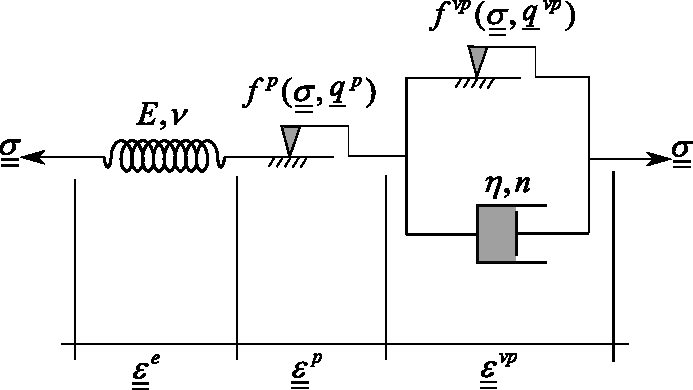
\includegraphics[scale = 1.0]{0510-representação reológica.pdf}
	\end{center}
	\caption{\label{modelo_reologico}Representação reológica do modelo elastoplástico-viscoplástico (adaptado de: \citeonline[p. 220]{Rousset1988})}
\end{figure}
Dessa forma, dentro das mesmas hipóteses dos modelos anteriores, a relação constitutiva linearizada fica sendo:
\begin{equation}
	\label{eq:lei_epvp}
	\dot \sigmall = \Dllll^{epvp}:\dot \varepsilonll = \Dllll:\dot \varepsilonll^e = \Dllll:\left(\dot \varepsilonll - \dot \varepsilonll^{p} - \dot \varepsilonll^{vp} \right).
\end{equation}

Uma observação importante é que as superfícies de escoamentos e as variáveis internas que definem a parcela elastoplástica e viscoplástica desse modelo podem ser diferentes entre si, incluindo a associação das suas respectivas funções potenciais com suas superfícies de escoamento. Apesar dessa abordagem genérica, na presente tese será adotada inicialmente a proposta seguida pelas soluções analíticas de \citeonline{Rousset1988} em que as forças termodinâmicas associadas às variáveis internas que governam a lei de endurecimento/amolecimento instantâneas e diferidas $\ql^p$ e $\ql^{vp}$, respectivamente, são funções multilineares de parâmetros coesivos em função da deformação plástica e viscoplástica equivalentes. Por exemplo para ilustrar esse comportamento, de forma unidimensional, segue-se as seguintes expressões \cite[p. 220]{Rousset1988}:
\begin{equation}
	\label{eq:qp_rousset}
	c(\varepsilon^p) = \left\{
		\begin{array}{lcl}
			2c - \dfrac{2(c-c_0)}{\varepsilon_0}\varepsilon^p \\ 
			2c_0~~~\text{se}~~~\varepsilon^p > \varepsilon_0
		\end{array}
	\right.
\end{equation}
que podem ser vistas graficamente na \autoref{lei_endurecimento_rousset}.
\begin{figure}[H]
	\begin{center}
		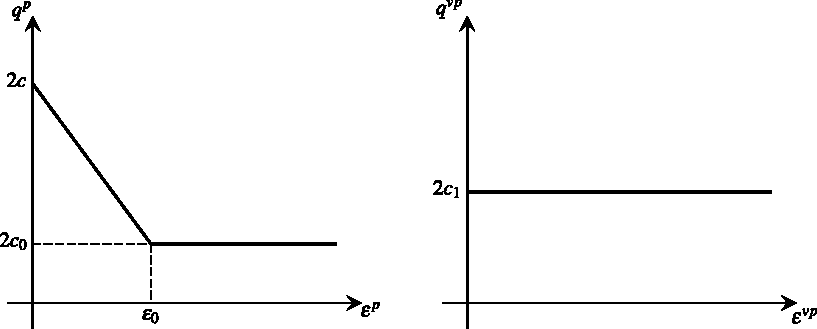
\includegraphics[scale = 1.0]{0511-lei de endurecimento ou amolecimento.pdf}
	\end{center}
	\caption{\label{lei_endurecimento_rousset}Leis de endurecimento e amolecimento para a parcela elastoplástica (à esquerda) e viscoplástica (à direita) (adaptado de: \citeonline[p. 220]{Rousset1988})}
\end{figure}
Nesse modelo, pode-se notar que a elastoplasticidade possui um amolecimento bilinear e a viscoplasticidade é perfeita. Os valores das coesões possuem a seguinte relação entre si: $c_0 < c_1 < c$. Essa relação não é arbitrária e pretende representar o inicio do comportamento diferido frente ao comportamento instantâneo. Essa desigualdade implica que as deformações viscoplásticas tenham inicio antes mesmo do maciço atingir sua resistência máxima de curto prazo e se mantém mesmo após o maciço ter atingido sua coesão residual. Generalizando para o caso tridimensional, para um determinado ponto no interior do maciço, tem-se, para seu estado de tensões, os domínios apresentados na \autoref{dominios_debernardi}.
\begin{figure}[H]
	\begin{center}
		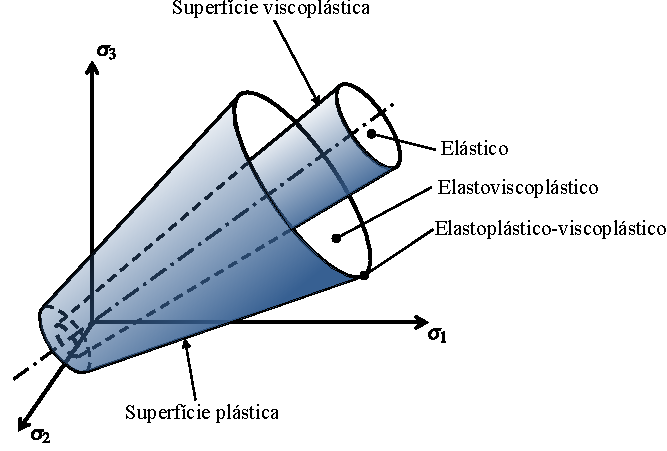
\includegraphics[scale = 1.0]{0512-dominios_superficie_epvp.pdf}
	\end{center}
	\caption{\label{dominios_debernardi}Domínios e superfícies do modelo elastoplástico-viscoplástico (adaptado de: \citeonline[p. 263]{Debernardi2009})}
\end{figure}
O comportamento desse modelo reológico pode ainda ser melhor entendido através da resposta das tensões frente a uma taxa de deformação constante. Esse comportamento é ilustrado na \autoref{resposta_epvp_deformacao_constante}, sendo $\dot \varepsilon_1 = \infty > \dot \varepsilon_2 > \dot \varepsilon_3 > \dot \varepsilon_4 = 0$.
\begin{figure}[H]
	\begin{center}
		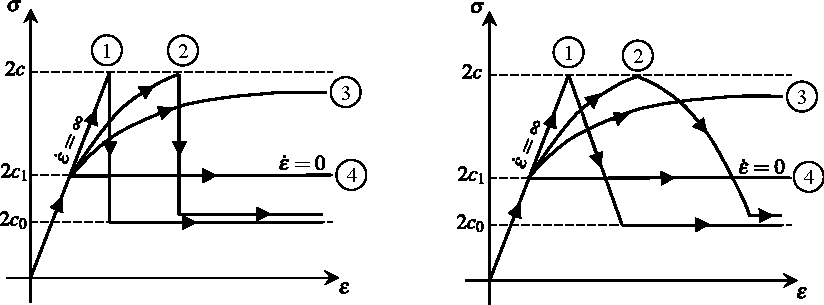
\includegraphics[scale = 1.0]{0513-resposta_epvp_deformacao_constante.pdf}
	\end{center}
	\caption{\label{resposta_epvp_deformacao_constante}Resposta do sistema a uma solicitação $\dot \varepsilon = \text{const}$ (adaptado de: \citeonline[p. 221]{Rousset1988})}
\end{figure}
Para altas taxas de deformação (caso 1 e 2), a tensão aumenta rapidamente até atingir o valor limite de $2c$ e em seguida diminui abruptamente (ruptura frágil) ou gradualmente (ruptura dúctil) mantendo uma tensão residual de $2c_0$. Pode-se notar que no caso 1, quando a taxa de deformação é muito alta, ao contrário do caso 2, os efeitos viscosos praticamente não ocorrem, tendo apenas o comportamento elastoplástico. Contudo, para taxas menores de deformação (caso 3) o limiar de ruptura não é atingido e a tensão evolui assintoticamente para um valor intermediário entre $2c$ e $2c_1$. Pode-se notar que no caso 4, quando a taxa de deformação é muito lenta, o modelo possui uma resposta elastoplástica perfeita com o limiar em $2c_1$.

% ----------------------------------------------------------
\chapter{Solução do modelo mecânico}
% ----------------------------------------------------------
A solução do modelo mecânico será feita através do \textit{software} ANSYS e a primeira parte desse capítulo descreverá a solução numérica pelo método dos elementos finitos (de forma mais genérica possível) comentando as opções do ANSYS, quando pertinente. Posteriormente, será dada ênfase na solução numérica envolvendo as do modelo constitutivo do material (que é o foco principal do trabalho). 

\section{Forma fraca das equações de campo}
No contexto da evolução quase estática e da hipótese das pequenas perturbações podem-se escrever as equações de campo na sua forma fraca através do princípio dos trabalhos virtuais. Sendo assim, aplicando um campo de deslocamento virtual $\dul$, cinematicamente admissível, em (\ref{eq:equilibrio_estatico_local}), porém ao longo de todo o volume $\Omega$ tem-se que:
\begin{equation}
	\label{eq:deslocamento_virtual}
	\int_{\Omega} \left(\divl \sigmall + \rho \fl \right)d\Omega \cdot \dul = 0,
\end{equation}
\begin{equation}
	\label{eq:deslocamento_virtual_2}
	\int_{\Omega} \divl \sigmall d\Omega \cdot \dul + \int_{\Omega} \rho \fl d\Omega \cdot \dul = 0.
\end{equation}

Aplicando o Teorema da Divergência no termo mais à esquerda da igualdade (\ref{eq:deslocamento_virtual_2}) obtém-se:
\begin{equation}
	\label{eq:deslocamento_virtual_3}
	\int_{\Omega} \sigmall : \dvarepsilonll d\Omega - \left(\int_{\Omega} \rho \fl \cdot \dul d\Omega + \int_{\partial \Omega} \Tl^d \cdot \dul dS \right) = U_{int} - W_{ext} = 0
\end{equation}

A expressão (\ref{eq:deslocamento_virtual}) é uma equação integral em que, no equilíbrio, o trabalho das forças externas $W_{ext}$ sobre o sistema é totalmente convertido em energia potencial interna $U_{int}$  de deformação.

\section{Notação de Voigt}
Os tensores simétricos de segunda e quarta ordem são comumente representados, respectivamente, por arranjos (\textit{arrays}) vetoriais e matriciais convenientes à álgebra computacional. Dessa forma é utilizada a seguinte notação \cite[p. 682]{Zienkiewicz2005}:
\begin{equation}
	\label{eq:sigmal}
	\sigmall \rightarrow \sigmal = \left\{\sigma_{11}~~~\sigma_{22}~~~\sigma_{33}~~~\sigma_{12}~~~\sigma_{23}~~~\sigma_{13} \right\}^T
\end{equation}
\begin{equation}
	\label{eq:varepsilonl}
	\varepsilonll \rightarrow \varepsilonl = \left\{\varepsilon_{11}~~~\varepsilon_{22}~~~\varepsilon_{33}~~~2\varepsilon_{12}~~~2\varepsilon_{23}~~~2\varepsilon_{13} \right\}^T
\end{equation}
\begin{equation}
	\label{eq:Dl}
	\Dllll \rightarrow \Dll = 
	\begin{bmatrix}
		D_{1111} & D_{1122} & D_{1133}  & D_{1112} & D_{1123} & D_{1113} \\
		D_{2211} & D_{2222}  & D_{2233}  & D_{2212} & D_{2223} & D_{2213}  \\
		D_{3311} & D_{3322} & D_{3333}  & D_{3312} & D_{3323} & D_{3313}  \\
		D_{1211} & D_{1222}	& D_{1233}  & D_{1212} & D_{1223} & D_{1213}  \\
		D_{2311} & D_{2322} & D_{2333} & D_{2312} & D_{2323} & D_{2313}  \\
		D_{1311} & D_{1322}	& D_{1333} & D_{1312} & D_{1323} & D_{1313} 
	\end{bmatrix}
\end{equation}
\begin{equation}
	\label{eq:dgdsl}
	\dgdsll \rightarrow \dgdsl = \left\{\dfrac{\partial g}{\partial \sigma_{11}}~~~\dfrac{\partial g}{\partial \sigma_{22}}~~~\dfrac{\partial g}{\partial \sigma_{33}}~~~\dfrac{\partial g}{\partial \sigma_{12}}~~~\dfrac{\partial g}{\partial \sigma_{23}}~~~\dfrac{\partial g}{\partial \sigma_{13}} \right\}^T
\end{equation}
\begin{equation}
	\label{eq:Uml}
	\Umll \rightarrow \Uml = \left\{1~~~1~~~1~~~0~~~0~~~0 \right\}^T
\end{equation}
\begin{equation}
	\label{eq:UmllotimesUll}
	\Umllll \rightarrow \Umll = 
	\begin{bmatrix}
		1 & 0 & 0 & 0 & 0 & 0 \\
		0 & 1 & 0 & 0 & 0 & 0  \\
		0 & 0 & 1 & 0 & 0 & 0  \\
		0 & 0 & 0 & 1/2 & 0 & 0  \\
		0 & 0 & 0 & 0 & 1/2 & 0  \\
		0 & 0 & 0 & 0 & 0 & 1/2 
	\end{bmatrix}
\end{equation}
\begin{equation}
	\label{eq:UmllotimesUll}
	\Umll \otimes \Umll \rightarrow  
	\begin{bmatrix}
		1 & 1 & 1 & 0 & 0 & 0 \\
		1 & 1 & 1 & 0 & 0 & 0  \\
		1 & 1 & 1 & 0 & 0 & 0  \\
		0 & 0 & 0 & 0 & 0 & 0  \\
		0 & 0 & 0 & 0 & 0 & 0  \\
		0 & 0 & 0 & 0 & 0 & 0 
	\end{bmatrix}
\end{equation}
sendo o subscrito $T$ a operação de transposição. Como se pode ver é utilizada a mesma simbologia de tensores de primeira ordem e de segunda ordem representando vetores (arranjos unidimensionais) e matrizes (arranjos bidimensionais), respectivamente. Nessa notação, as operações também são transformadas, de tal forma que:
\begin{equation}
	\label{eq:operacoes_voigt}
	\begin{array}{lcl}
		\underline{a} \cdot \underline{b} \rightarrow \underline{b}^T \underline{a}, \\ 
		\underline{\underline{a}} : \underline{\underline{b}} \rightarrow \underline{a}^T \underline{b}, \\ 
		\underline{\underline a} \otimes \underline{\underline b} \rightarrow \underline a ~ \underline b ^T, \\ 
		\underline{\underline{\underline{\underline{C}}}} : \underline{\underline{b}} \rightarrow \underline{\underline C} ~ \underline b, \\ 
		\underline{\underline{b}}:\underline{\underline{\underline{\underline{C}}}} : \underline{\underline{b}} \rightarrow \underline {b}^T \underline{\underline{C}} ~ \underline{b}, \\ 
		\left( 	\underline{\underline{\underline{\underline{C}}}}:\underline{\underline{a}} \right) \otimes \left( \underline{\underline{b}} :	\underline{\underline{\underline{\underline{C}}}} \right) \rightarrow \underline{\underline{C}}~ \underline{a}~\underline{b}^T \underline{\underline{C}}.
	\end{array}
\end{equation}

Essa será a notação adotada para o restante do trabalho. Logo, o teorema dos trabalhos virtuais (\ref{eq:deslocamento_virtual_3}) pode ser reescrito da seguinte forma:
\begin{equation}
	\label{eq:deslocamento_virtual_3}
	\int_{\Omega} \dvarepsilonl^T \sigmal d\Omega - \left(\int_{\Omega} \rho \dul^T \fl d\Omega + \int_{\partial \Omega} \dul^T \Tl^d dS \right) = U_{int} - W_{ext} = 0
\end{equation}
\section{Discretização espacial em elementos finitos}
\label{cap:Discretização espacial em elementos finitos}
A solução por elementos finitos consiste em discretizar o domínio $\Omega$ em um conjunto de elementos contíguos $\Omega_e$, estabelecendo o que se chama de malha de elementos finitos (\autoref{discretizacao_MEF}). Cada elemento da malha tem um formato simples: linha, triângulo ou quadrilátero, tetraedro ou hexaedro, dependendo da dimensão (1D, 2D ou 3D) do domínio a ser discretizado. Cada elemento está conectado a outros elementos compartilhando "nós" sendo que a principal incógnita do problema são os deslocamentos nodais.
\begin{figure}[H]
	\begin{center}
		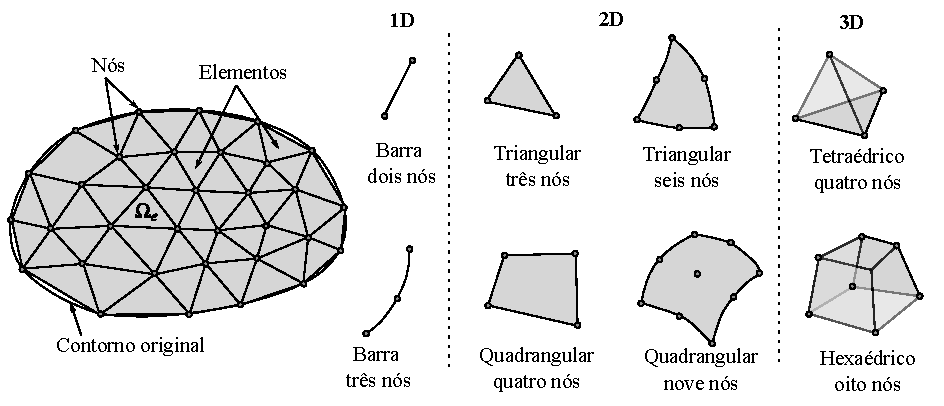
\includegraphics[scale = 1.0]{0601-discretizacao_dominio.pdf}
	\end{center}
	\caption{\label{discretizacao_MEF}Discretização de um domínio genérico em elementos finitos (adaptado de: \citeonline[p. 1-2]{DeSouza2003})}
\end{figure}

Nesse método, o campo de deslocamentos no interior dos elementos é relacionado com os deslocamentos nodais através de funções de interpolação, por exemplo, lineares ou quadráticas, cujos coeficientes são postos em função dos deslocamentos nodais. Dessa forma, o campo de deslocamentos no interior do elemento pode ser descrito como:
\begin{equation}
	\label{eq:campo_deslocamentos}
	\ul(\xl) = \ul(x_1,x_2,x_3) = \Nll(\xl)\ul_e.
\end{equation}
sendo $\ul(\xl)$ o campo de deslocamentos no interior do elemento, $\ul_e$ os deslocamentos nodais e $\Nll$ a matriz contendo as funções de interpolação (também conhecidas como funções de forma). A matriz $\Nll$  tem a seguinte estrutura:
\begin{equation}
	\label{eq:matriz_N}
	\Nll = 	\begin{bmatrix}
		N_1 & 0 & 0 & N_2 & 0 & 0 &  	& N_{n_e} & 0 & 0 \\
		0 & N_1 & 0 & 0 & N_2 & 0 & ... & 0 & N_{n_e} & 0  \\
		0 & 0 & N_1 & 0 & 0 & N_2 &  	& 0 & 0 & N_{n_e} 
	\end{bmatrix}_{n_d \times (n_e \cdot n_d)}
\end{equation}
em que $N_i$ são as funções de interpolação de cada nó $i$, $n_e$ número de nós do elemento e $n_d$ o número de dimensões. Introduzindo (\ref{eq:campo_deslocamentos}) nas equações de compatibilidade (\ref{eq:green_lagrange_linearizado}) tem-se:
\begin{equation}
	\label{eq:deformacoes}
	\varepsilonl(\xl) = \varepsilonl(x_1,x_2,x_3) = \nabla^s\ul(\xl) = \nabla^s \Nll~\ul_e = \Bll~\ul_e
\end{equation}
sendo $\varepsilonl$ o campo de deformações e $\Bll = \nabla^s \Nll$ a matriz que relaciona os deslocamentos nodais com as deformações no interior do elemento. Para problemas tridimensionais, o operador gradiente simétrico $\nabla^s$, na notação de Voigt, é dado por:
\begin{equation}
	\label{eq:gradiente_simetrico}
	\nabla^s = 	\begin{bmatrix}
		\dfrac{\partial}{\partial x_1} & 0 & 0  \\
		0 & \dfrac{\partial}{\partial x_2} & 0  \\
		0 & 0 & \dfrac{\partial}{\partial x_3} \\
		\dfrac{\partial}{\partial x_2} & \dfrac{\partial}{\partial x_1} & 0 \\
		0 & \dfrac{\partial}{\partial x_3} & \dfrac{\partial}{\partial x_2} \\
		\dfrac{\partial}{\partial x_3} & 0 & \dfrac{\partial}{\partial x_1}		
	\end{bmatrix}_{n_c \times n_d}
\end{equation}
em que $n_c$  é o número de componentes de deformações. Introduzindo (\ref{eq:deformacoes}) na lei de comportamento do material, é possível determinar as tensões no interior do elemento também em função dos deslocamentos nodais:
\begin{equation}
	\label{eq:tensoes}
	\sigmal(\xl) = \sigmal(x_1,x_2,x_3) = \Dll ~ \Bll ~\ul_e + \Dll ~\varepsilonl_0 + \sigmal_0
\end{equation}
na qual $\varepsilonl_0$ e $\sigmal_0$ são deformações e tensões iniciais no interior do elemento, respectivamente. Nos problemas de túneis, é através de $\sigmal_0$ que é introduzido as tensões \textit{in situ}. Para o caso de tensão geostática hidrostática, em um túnel de profundidade $H$ em um maciço com peso específico $\gamma_m$ a seguinte expressão é utilizada:
\begin{equation}
	\label{eq:tensoes_iniciais}
	\sigmal_0 = \gamma_m H \Uml
\end{equation}

Introduzindo as expressões (\ref{eq:campo_deslocamentos}), (\ref{eq:deformacoes}) e (\ref{eq:tensoes}) no princípio dos trabalhos virtuais (\ref{eq:deslocamento_virtual_3}), considerando o domínio de um elemento $\Omega_e$, obtém-se a seguinte equação de equilíbrio em forças:
\begin{equation}
	\label{eq:forcas_interna_externa}
	\Fl_{int_e} - \Fl_{ext_e} = \underline 0
\end{equation}
em que:
\begin{equation}
	\label{eq:forca_interna}
	\Fl_{int_e} = \int_{\Omega_e} \Bll^T \sigmal d\Omega_e = \Kll_e \ul_e + \Fl_{\varepsilon_{0_e}} + \Fl_{\sigma_{0_e}}
\end{equation}
\begin{equation}
	\label{eq:forca_externa}
	\Fl_{ext_e} = \Fl_{V_e} + \Fl_{S_e} + \Fl_{C_e} + \Fl_{N_e}
\end{equation}
nos quais:
\begin{equation}
	\label{eq:elementos_forca_interna}
	\Kll_e = \int_{\Omega_e} \Bll^T \sigmal d\Omega_e,~~~ \Fl_{\varepsilon_{0_e}} = \int_{\Omega_e} \Bll^T \Dll~ \varepsilonl_0 d\Omega_e,~~~ \Fl_{\sigma_{0_e}} = \int_{\Omega_e} \Bll^T \sigma_0 d\Omega_e,
\end{equation}
\begin{equation}
	\label{eq:elementos_forca_externa}
	\Fl_{V_e} = \int_{\Omega_e} \rho \Nll^T \fl d\Omega_e,~~~ \Fl_{S_e} = \int_{\partial \Omega_e} \Nll^T \Tl^d dS_e,~~~
	\Fl_{C_e} = \int_{\partial \Omega_{e}} \Nll^T \Tl^c dS_c,
\end{equation}
sendo que $\Fl_{int_e}$ e $\Fl_{ext_e}$ são as forças internas e externas no elemento, respectivamente, $\Kll_e$ a matriz de rigidez do elemento, $\Fl_{\varepsilon_{0_e}}$ e $\Fl_{\sigma_{0_e}}$  forças internas no elemento devido às deformações inciais e tensões iniciais, respectivamente, $\Fl_{V_e}$ forças de volume do elemento, $\Fl_{S_e}$ forças de superfície no contorno livre do elemento, $\Fl_{C_e}$ forças de contato entre elementos vizinhos e $Fl_{N_e}$  forças nodais. A Figura 6.2 ilustra as forças externas de um elemento genérico.
\begin{figure}[H]
	\begin{center}
		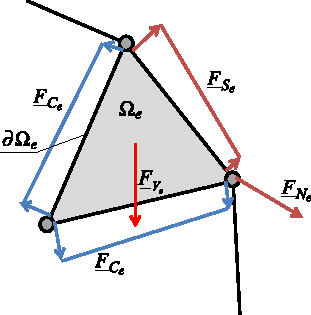
\includegraphics[scale = 1.0]{0602-diagrama de corpo livro de um elemento finito.pdf}
	\end{center}
	\caption{\label{discretizacao_MEF}Diagrama de corpo livre de um elemento finito (adaptado de: \citeonline[p. 19]{Lizarza2011})}
\end{figure}
No método dos elementos finitos, as integrais de volume no domínio  $\Omega_e$, por eficiência, são geralmente resolvidas em um domínio de referência $\Omega_\xi$ com geometria normalizada $-1 \le \xi_i \le 1$. As coordenadas $\underline \xi$ também são conhecidas como coordenadas naturais do elemento. Portanto, é feita a seguinte troca de variáveis nas integrais de volume \cite[p. 147]{Zienkiewicz2005}:
\begin{equation}
	\label{eq:troca_variavel_integral_volume}
	\int_{\Omega_e}d\Omega_e = \iiint dx_1 dx_2 dx_3 = \int_{\Omega_\xi}det(\Jll)d\Omega_\xi = \int_{-1}^{1}\int_{-1}^{1}\int_{-1}^{1}\text{det}(\Jll)d\xi_1d\xi_2d\xi_3
\end{equation}
em que $\Jll = \dfrac{\partial \xl}{\partial \xil}$  é o Jacobiano da transformação entre as coordenada $\xl$ e $\xil$, sendo calculado com as mesmas funções de interpolação usadas para os deslocamentos no interior do elemento, se tratando, portanto, de um \textbf{elemento isoparamétrico}. A integral assim representada é então resolvida pelo método da Quadratura de Gauss-Legendre. Portanto, para uma função $f(\xl)$ qualquer, no domínio $\Omega_e$, tem-se:
\begin{equation}
	\label{eq:troca_variavel_integral_volume}
	\int_{\Omega_e}f(\xl)d\Omega_e = \int_{-1}^{1}\int_{-1}^{1}\int_{-1}^{1}f(\xil)\text{det}(\Jll)d\xi_1d\xi_2d\xi_3 = \sum_{i_p=1}^{n_p}W_{i_p}J_{i_p}f(\xil_{i_p})
\end{equation}
em que $n_p$ é o número de pontos de integração (ou pontos de Gauss), $W_{i_p}$ é o peso referente ao ponto de integração, $f(\xil_{i_p})$ é o valor da função nas coordenadas naturais do ponto de integração e $J_{i_p}$ é o determinante do Jacobiano da transformação (nas coordenadas do ponto de integração) dado por \cite[p. 206-207]{Zienkiewicz2005}:
\begin{equation}
	\label{eq:jacobiano_transformacao}
	J_{i_p} = \left\{
	\begin{array}{lcl}
		 \text{det}(\Jll)_{i_p}~~~\text{em 3D e estado plano de deformações} \\
		2\pi\xi_{r_{i_p}}\text{det}(\Jll)_{i_p} ~~~\text{em axissimetria}
	\end{array}
\right..
\end{equation}
sendo $\xi_{r_{i_p}}$ a coordenada radial natural do ponto de Gauss. A equação (6.26) integra  exatamente se este for um polinômio de ordem menor ou igual a $2n_p-1$.

Os elementos finitos que serão utilizados nesse trabalho com suas funções de interpolação, pesos e coordenadas dos pontos de integração podem ser vistos na \autoref{PLANE183}, para análises em estado plano de deformações e axissimetria e, para análises tridimensionais, que consomem maior tempo de processamento, será utilizado o elemento da \autoref{SOLID185}.
\begin{figure}[H]
	\begin{center}
		\includegraphics[scale = 1.0]{0603-quadrilatero quadratico.pdf}
	\end{center}
	\caption{\label{PLANE183}Funções de interpolação, pesos e coordenadas dos pontos de Gauss para o elemento quadrilátero quadrático \textit{serendipity} isoparamétrico (adaptado de: \citeonline[p. 337, 369-370]{ANSYS2018})}
\end{figure}
\begin{figure}[H]
	\begin{center}
		\includegraphics[scale = 1.0]{0604-hexaedro linear.pdf}
	\end{center}
	\caption{\label{SOLID185}Funções de interpolação, pesos e coordenadas dos pontos de Gauss para o elemento hexaedro trilinear isoparamétrico (adaptado de: \citeonline[p. 345, 369-370]{ANSYS2018})}
\end{figure}

No ANSYS, ambos elementos possuem a opção degenerada em que é possível trabalhar de forma colapsada, triangular, por exemplo, no caso do PLANE183, e prisma, tetraédrica ou piramidal, no caso do SOLID185. Nas análises não serão utilizadas essas formas. 

O elemento SOLID185 possuí também opções que lidam com problemas de travamento (\textit{Locking}) e modos espúrios (\textit{Hourglass}). O travamento é caracterizado por uma rigidez excessiva do elemento, e ocorre principalmente em elementos de primeira ordem com integração completa que estão sujeitos a flexão. Ou ainda, quando o material é quase incompressível. Também podem ocorrer em elementos de segunda ordem, quando as deformações plásticas são da ordem das deformações elásticas. Esse problema evita-se com refinamento da malha, técnicas de subintegração e funções de formas extras. O ANSYS possuí as duas últimas técnicas para o SOLID185 (\textit{Uniform Reduced Integration with Hourglass Control} e \textit{Enhanced Strain Formulation}). Os modos espúrios ocorrem quando se utiliza as técnicas de subintegração e é caracterizado por uma distorção no elemento porém com zero deformação. Esse problema é evitado utilizando integração completa ou refinamento da malha. No presente trabalho se utilizará a \textbf{integração completa} (\textit{Full integration with B method}) e se tentará evitar esses problemas através do \textbf{refinamento da malha}. 

\section{Solução do sistema não linear}
\label{cap: solução do sistema}

Após o processo de discretização do domínio $\Omega$ é necessário fazer a montagem e a solução do seguinte sistema global de equações:
\begin{equation}
	\label{eq:sistema_global}
	\left(\Kll~\ul + \Fl_{\varepsilon_{0}} + \Fl_{\sigma_{0}}\right) - \left(\Fl_V+\Fl_S+\Fl_N \right) = \Fl_{int} - \Fl_{ext} = f(\ul) = \underline{0}  
\end{equation}
em que $\Kll$ é a matriz de rigidez global resultante da montagem das matrizes de rigidezes $\Kll_e$ de cada elemento, $\ul$ é o vetor incógnito de deslocamentos nodais global proveniente da montagem dos deslocamentos nodais $\ul_e$ de cada elemento, $\left\{\Fl_V,\Fl_S,\Fl_N,\Fl_{\varepsilon_0},\Fl_{\sigma_0} \right\}$ são as forças globais resultantes da montagem das forças em cada elemento, conforme (\ref{eq:elementos_forca_interna}) e (\ref{eq:elementos_forca_externa}). Evidentemente não há um vetor de forças de contato global $\Fl_C$, uma vez que as forças de contato entre elementos vizinhos possuem a mesma magnitude e sentidos contrários e, portanto, se anulam no somatório global.

Quando há uma não linearidade envolvendo as leis constitutivas do material (tal como na plasticidade ou viscoplasticidade, em que o problema é dependente da trajetória das tensões), a matriz de coeficientes $\Kll$ passa a depender dos deslocamentos nodais incógnitos  $\ul$, tornando o sistema (\ref{eq:sistema_global}) não linear. O \textbf{método de Newton-Raphson} (NR) é o processo iterativo comumente utilizado para resolver esse sistema e é utilizado pelo ANSYS. Dessa forma, aproximando (\ref{eq:sistema_global}) por uma série de Taylor truncada na primeira ordem (linearização) tem-se:
\begin{equation}
	\label{eq:taylor}
	\fl(\ul) \approx \fl(\ul_i) + \fl'(\ul_i)(\ul_{i+1}-\ul_i).
\end{equation}

Fazendo $\fl(\ul) = \underline{0}$, isolando $\ul_{i+1}$ e substituindo (\ref{eq:sistema_global}) em (\ref{eq:taylor}), considerando que $\Fl_{ext}$ não depende dos deslocamentos (devido à hipótese das pequenas perturbações), tem-se a seguinte expressão iterativa para aproximar $\ul$:
\begin{equation}
	\label{eq:NR}
	\ul_{i+1} = \ul_i - \Kll(\ul_i)^{-1}\left(\Fl_{int}(\ul_i)-\Fl_{ext} \right) = \ul_i - \Kll_i^{-1} \left(\Fl_{int_i} - \Fl_{ext} \right) = \ul_i + \Kll_i^{-1}\Rl_i = \ul_i + \Delta \ul_i
\end{equation}
em que $\Delta \ul_i$ é o incremento de deslocamentos nodais da iteração atual $i$, $\Fl_{int_i}$ são as forças internas (ou forças restauradoras) da iteração atual (calculadas com $\ul_i$), $\Rl_i$ é o vetor de carga desbalanceado (também chamado de resíduo) para a iteração atual, $\Kll_i$ a matriz de rigidez global tangente na iteração atual, $\ul_i$ os deslocamentos nodais na iteração atual e $\ul_{i+1}$ os deslocamentos nodais atualizados para a próxima iteração.

Como $\Delta \ul_i = \Kll_i^{-1}\Rl_i$ é um sistema de equações esparso (contém muitos elementos nulos) e geralmente simétrico, há diversas técnicas de solução que buscam explorar essas características para obter eficiência computacional. O ANSYS possui uma técnica de \textbf{solução direta}, que busca resolver o sistema através de operações que compreendem a inversão da matriz de rigidez, e três técnicas de \textbf{soluções indiretas}, que se aproximam da solução do sistema de forma interativa com uma dada tolerância.

A solução direta (\textit{SPARSE - Sparse Direct Solver}) consiste em aplicar a fatorização de Cholesky modificada $\Kll = \Lll~\Dll~ \Lll^T$ (em que $\Lll$ é uma matriz triangular inferior e $\Dll$ uma matriz diagonal) e, através de substituições progressivas e retroativas, resolver o sistema. Em geral, para problemas com poucos graus de liberdade, é uma solução bastante eficiente e não possui problemas de instabilidade numérica. Algoritmos de solução direta análogas podem ser encontrados em \citeonline{Felippa1975} e \citeonline{Smith2014}.

As soluções indiretas, implementadas no ANSYS, se baseiam na família de Métodos dos Gradientes Conjugados Pré-Condicionados, que consistem em minimizar o potencial $V(\Delta \ul) = \frac{1}{2}\Delta \ul^T\Kll~\Delta \ul - \Delta \ul^T\Rl$ com aproximações $\Delta \ul^{(j+1)}=\Delta \ul^{j} + a_j \underline{d}^{(j)}~\text{para}~j=0,1,2,..m$, sendo $\underline d^{(j)}$ os gradientes conjugados, ou seja, $\underline {d}^{{(i)}^T} \Kll d^{(j)} = 0,~~ \forall i \neq j$. Quando o sistema é bem condicionado, sua solução converge para $m \leq n_{gdl}$ iterações e o número de operações é proporcional à raiz quadrada do número de condição da matriz $\Kll$, numero este que é a razão entre o maior e menor autovalor da matriz $\Kll$. Em vista disso, há diversas técnicas de transformação do sistema para melhorar o condicionamento dessa matriz através de uma transformação do tipo $\Mll^{-1}\Kll~\ul = \Mll^{-1} \Rl$, em que $\Mll$ é o pré-condicionador. O ANSYS possuí três métodos implementados \cite[p. 647]{ANSYS2018}:

\begin{alineas}
	
	\item JCG (\textit{Jacobi Conjugate Gradiente}): o pré-condicionador é tomado como sendo uma matriz diagonal cujos termos são as diagonais da matriz de rigidez;
	
	\item ICCG (\textit{Incomplete Cholesky Conjugate Gradiente}), o pré-condicionador é tomado através de uma fatorização incompleta de Cholesky. O algoritmo é internamente desenvolvido pela ANSYS e não publicado, e é mais robusto que o primeiro para matrizes mal condicionadas;
	
	\item PCG (\textit{Preconditioned Conjugate Gradiente}) é um solucionador da \textit{Computational Applications and System Integration, Inc} que não consta nos manuais do \textit{software}. Contudo, é dito eficiente e confiável para problemas mal condicionados.
	
\end{alineas}

Maiores explicações dessas soluções indiretas, podem ser encontrados em \citeonline[p. 316]{Mendonca2019}. Cabe salientar que, tanto os métodos diretos quanto indiretos, são implementados buscando a eficiência computacional, evitando-se trabalhar com os elementos nulos, diminuindo o armazenamento e o número de operações. Alguns métodos que compreendem reordenamento e armazenamento eficiente do sistema, utilizados pelo ANSYS, podem ser encontrados em \citeonline{George1981}. Além disso, uma vantagem do ANSYS é a possibilidade de trabalhar com computação de alto desempenho (\textit{High Performance Computing}) com opções de aceleração usando placas de vídeo da Nvidia, memória compartilhada (SMP - \textit{Shared-Memory Parallel}) ou computação distribuída (MPI - \textit{Message Passing Interface}). Para o presente trabalho, foi utilizado a opção de SMP com 12 processadores.

A rigor para um problema não linear a escolha do melhor método de solução vai depender de testagem. Por padrão o ANSYS utiliza o SPARSE. Contudo, recomenda utilizar o método PCG para estruturas sólidas 3D que possuem mais de 200.000 graus de liberdade. Para problemas mal condicionados, seja pela forma dos elementos, grandes diferenças entre as propriedades dos materiais ou ainda por insuficiente condições de contorno, recomenda-se o SPARSE \cite[p. 242]{ANSYS2018b}. Esse foi o método de solução escolhido para o presente trabalho.

Para incorporar a dependência do histórico de cargas/tempo, para um dado passo de carga/tempo $p$, a expressão (\ref{eq:NR}) é discretizada em $1 \leq n \leq n_s$ subpassos em que a carga externa e o tempo do passo são incrementados linearmente. Dessa forma, itera-se o sistema (\ref{eq:NR}) repetidas vezes para cada subpasso $n$ tendo-se:
\begin{equation}
	\label{eq:NR1}
	\Delta \ul_{n,i} = \Kll_{n,i}^{-1}\left(\Fl_{ext_{n}} - \Fl_{int_{n,i}} \right) = \Kll_{n,i}^{-1}\Rl_{n,i},
\end{equation}
\begin{equation}
	\label{eq:NR2}
	\ul_{n,i+1} = \ul_{n,i}+\Delta\ul_{n,i},
\end{equation}
\begin{equation}
	\label{eq:NR3}
	\Fl_{ext_{n}} = \Fl_{ext_{n-1}} + \Delta \Fl_{p},
\end{equation}
\begin{equation}
	\label{eq:NR4}
	t_{n} = t_{n-1} + \Delta t_p,
\end{equation}
em que
\begin{equation}
	\label{eq:NR5}
	\Fl_{int_{n,i}} = \left( \int_{\Omega} \Bll^T \sigmal d\Omega \right)_{n,i}
\end{equation}
sendo $\ul_{0,0}$, $\Fl_{int_{0,0}}$, $\Fl_{ext_0}$   e $t_0$ nulos. Para os próximos subpassos os valores de $\ul_{n,0}$ e $\Fl_{int_{n,0}}$, correspondem aos valores da solução convergente no subpasso anterior $n-1$. O número de subpassos $n_s$ e o incremento de força externa $\Delta \underline{F}_p$ são dependentes do incremento de tempo utilizado no passo $\Delta t_p$, e são dados por:
\begin{equation}
	\label{eq:NR6}
	n_s = \dfrac{t_p}{\Delta t_p},~~~ \Delta \Fl_{p} = \dfrac{\Fl_{ext_p}}{n_s}
\end{equation}
sendo $t_p$ e $\Fl_{ext_p}$, nessa ordem, o tempo e a força no final do passo. Em busca da convergência e eficiência computacional, o ANSYS tem a opção de variar automaticamente o $\Delta t_p$ dentro de um intervalo $\Delta t_{p_{min}} \leq \Delta t_p \leq \Delta t_{p_{max}}$ fornecido pelo usuário. É possível que o algoritmo não convirja em um dado subpasso durante as iterações e, portanto, é utilizado um limite de $n_{eqit} = 25$ iterações de equilíbrio por subpasso. Quando a solução não converge dentro desse limite, o ANSYS divide pela metade o incremento de tempo, e consequentemente a carga, e reinicia o cálculo do passo. Esse procedimento é chamado de Método da Bisseção e é executado tantas vezes quanto necessárias até atingir a convergência ou $\Delta t_p \leq \Delta t_{p_{min}}$ a partir do qual a solução é dada como não convergente e estabelecido o critério de parada \cite[p. 637]{ANSYS2018}.

A convergência é verificada sobre o vetor resíduo e o incremento de deslocamentos nodais para cada iteração de equilíbrio, através das seguintes expressões (omitindo-se o subíndice $n$) \cite[p. 667]{ANSYS2018}:
\begin{equation}
	\label{eq:convergencia}
	||\Rl_i|| \leq \varepsilon_R R_{ref},~~~ ||\Delta \ul_i || \leq \varepsilon_u u_{ref}
\end{equation}
em que $\varepsilon_R$ e $\varepsilon_u$ são as tolerâncias para o resíduo (de 0,5\%) e deslocamentos (de 5\%), respectivamente. Os valores de referência $R_{ref}$ e $u_{ref}$ são $||\Fl_{ext_p}||$ e $||\ul_{n,i}||$, respectivamente. Ou seja, por padrão o critério para o resíduo é de 0,5\% do valor das forças externas e os deslocamentos não podem apresentar uma variação maior do que 5\%. No ANSYS, a norma pode ser calculada de três formas: a máxima componente em valor absoluto, a soma absoluta das componentes ou a norma euclidiana das componentes, conforme:
\begin{equation}
	\label{eq:jacobiano_transformacao}
	||\underline *|| = \left\{
	\begin{array}{lcl}
		||\underline *||_\infty = \text{max}(*_j) \\
		||\underline *||_1 = \sum_{j}|*_j| \\
		||\underline *||_2 = (\sum_{j}*_j^2)^{1/2}
	\end{array}
	\right..
\end{equation}
em que $j$ é o índice da componente do vetor $\underline * = \Rl$ ou $\underline * = \Delta \ul$. Para o presente trabalho foi escolhida a norma euclidiana para o resíduo e a norma infinita para o incremento de deslocamento. Essas opções já eram o padrão do ANSYS. A \autoref{NR} ilustra o andamento da solução ao longo dos subpassos. Pode-se ver, caso haja a convergência entre os subpassos, que o resíduo e o incremento de deformações vão ficando cada vez menores ao longo das iterações de equilíbrio.
\begin{figure}[H]
	\begin{center}
		\includegraphics[scale = 1.0]{0605_2-ilustracao das iteracoes do método de NR.pdf}
	\end{center}
	\caption{\label{NR}Ilustração das iterações do método de Newton-Raphson (adaptado de: \citeonline[p. 301]{Chen1988})}
\end{figure}

O ANSYS possui ainda quatro variações do método de Newton-Raphson de acordo com a estratégia de atualização da matriz de rigidez $\Kll_{n,i}$ (\citeyear{ANSYS2018}, p. 666): 
\begin{alineas}
	
	\item \textbf{Completo} (\textit{Full}): quando a matriz de rigidez é atualizada a cada iteração $i$, ou seja, $\Kll_{n,i} \leftarrow \Kll_{n,i}$. Essa opção reduz o número de iterações de equilíbrio (convergência quadrática), porém, exige a montagem, fatorização e inversão da matriz a cada iteração;
	
	\item \textbf{Modificado} (\textit{Modified}): quando a matriz de rigidez é atualizada apenas a cada subpasso de carga/tempo $n$, ou seja, $\Kll_{n,i} \leftarrow \Kll_{n,0}$; 
	
	\item \textbf{Inicial} (\textit{Inicial Stiffness}): quando é utilizada a mesma matriz para todos os subpassos e iterações, ou seja, $\Kll_{n,i} \leftarrow \Kll_{0,0}$. 
	
	\item \textbf{Completo Assimétrico} (\textit{Full unsymmetric}): é a mesma opção da Completo porém monta a matriz de rigidez não a considerando simétrica.
	
\end{alineas}

A convergência quadrática da opção de Newton-Raphson Completo só é efetivamente obtida se for utilizado o módulo consistente $\Dll^{alg}$ após o algoritmo de integração das tensões, conforme \citeonline{Simo1985}. A opção de Newton-Raphson Completo Assimétrico é importante para os casos em que se calcula o módulo consistente e se tem plasticidade não associada. A plasticidade não associada pode levar a módulos constitutivos não simétricos e pode não convergir com o Newton-Raphson Completo, pois este monta a matriz de rigidez considerando-a simétrica. Uma forma de contornar esse problema é não utilizar o módulo consistente, porém será necessária mais iterações de equilíbrio para a convergência. Nessa tese, como será visto mais adiante, foi programado o módulo constitutivo consistente, mas o seu uso é opcional.

Apesar de não terem sido utilizadas nessa tese, o ANSYS possui ainda quatro técnicas para melhorar a convergência do método de Newton-Raphson em problemas estáticos, que são \cite[p. 668-673]{ANSYS2018}:

\begin{alineas}
	\item \textbf{Preditor} (\textit{Predictor}): extrapola o vetor de deslocamentos iniciais de cada subpasso utilizando os incrementos de deslocamentos acumulados do subpasso anterior multiplicados pela relação entre os incrementos de tempo de ambos subpassos;
	
	\item \textbf{Descida Adaptativa} (\textit{Adaptative Descent}): consiste em alternar entre a matriz de rigidez tangente e secante conforme o andamento do resíduo durante as iterações de equilíbrio. Só é utilizada em conjunto com o método de Newton-Raphson Completo;
	
	\item \textbf{Pesquisa de linha} (\textit{Line Search}): tenta melhorar a solução multiplicando o incremento de deslocamentos por um escalar determinado pela minimização da energia do sistema;
	
	\item \textbf{Método do comprimento de arco} (\textit{Arc-Length Method}): utilizado para solução de equilíbrio estático não-linear de problemas instáveis como flambagem e pós-flambagem.	
\end{alineas}

Na \autoref{NR-fluxograma} tem-se o fluxograma do método de Newton-Raphson, mostrando as três opções de atualização da matriz de rigidez, o método da bisseção e os laços das iterações de equilíbrio e de subpassos.
\begin{figure}[H]
	\begin{center}
		\includegraphics[scale = 1.0]{0606_2-fluxograma do metodo NR.pdf}
	\end{center}
	\caption{\label{NR-fluxograma}Fluxograma do método de Newton-Raphson para solução do sistema de equações globais não lineares}
\end{figure}
Ainda na \autoref{NR-fluxograma} está detalhado a parte de atualização das tensões, variáveis internas e do módulo constitutivo, que serão os temas do próximo capítulo. É importante nesse fluxograma o detalhe dos laços nos elementos e pontos de Gauss, pois a customização do modelo do material, através da subrotina \textit{Usermat} está justamente aninhado nesse laço mais interno dos pontos de Gauss.

\section{Algoritmo de atualização das tensões e variáveis internas}

Como visto no capítulo anterior, durante as iterações de equilíbrio é necessário fazer a integração espacial das forças internas no contexto do método dos elementos finitos. Essa integração pode ser escrita da seguinte maneira:
\begin{equation}
	\label{eq:Fint}
	\Fl_{int_{n,i}} = \int_{\Omega}\Bll^T\sigmal_{n}d\Omega = \sum_{i_e=1}^{n_e}\sum_{i_p=1}^{n_p}\left( \Bll^T\sigmal_{n}WJ\right)_{i_p,i_e}
\end{equation}
sendo $\sigmal_{n}$ dado pela relação constitutiva do material. Contudo, as relações constitutivas, por dependerem da trajetória das tensões e/ou do tempo, estão descritas em forma de taxas, conforme visto no \autoref{cap: modelo mecanico}. E, portanto, é necessária a solução desse sistema de equações diferenciais ordinárias por algum método de integração juntamente com as iterações de equilíbrio. Essa etapa de integração, no esquema de elementos finitos, é conhecida como \textbf{algoritmo de atualização das tensões e variáveis internas}. Tal como ilustrado na \autoref{NR-fluxograma}, esse algoritmo ocorre para cada ponto de Gauss de cada elemento e tem por finalidade obter o incremento de tensão $\Delta \sigmal$ e de forças associadas às variáveis internas $\Delta \ql$ através do incremento de deformação total $\Delta \varepsilonl$ do subpasso.

\subsection{Integração das equações constitutivas elastoplásticas}

Como visto no \autoref{cap: modelo mecanico}, considerando a hipótese das pequenas transformações, as equações constitutivas da elastoplasticidade, já na notação de Voigt, podem ser escritas como:
\begin{equation}
	\label{eq:constitutiva_ep}
	\left\{
	\begin{array}{lcl}
		\dot \sigmal = \Dll~\dot \varepsilonl^e = \Dll(\dot \varepsilonl - \dot \varepsilonl^p) \\
		\dot \varepsilonl^p = \dot \lambda \dgdsl \\
		\dot \ql = \dot \lambda \hl \\
		\dot f = \dfdsl^T \dot \sigmal + \dfdql^T \dot \ql = 0 \\
		f \leq 0,~~\dot \lambda \geq 0,~~\dot \lambda f = 0	
	\end{array}
	\right..
\end{equation}

Em geral, a proposta dos algoritmos de integração consiste em integrar as equações constitutivas através de métodos numéricos, como os de Runge-Kutta, com técnicas explícitas, implícitas ou semi-implícitas. E dessa forma, conhecido o conjunto de $\left\{ \varepsilonl_n, \varepsilonl_n^p,\sigmal_n,\ql_n \right\}$ do último subpasso convergido $n$ e o incremento de deformação total acumulado $\Delta \varepsilonl$ obtido pela iteração de Newton-Raphson, busca-se os valores $\left\{ \varepsilonl_{n+1}, \varepsilonl_{n+1}^p,\sigmal_{n+1},\ql_{n+1} \right\}$, plasticamente admissíveis, do subpasso $n+1$. No presente trabalho \textbf{será implementado um esquema semi-implícito de Euler de dois passos para a relação constitutiva elastoplástica}, inicialmente em elastoplasticidade perfeita, e posteriormente com a lei de endurecimento/amolecimento multilinear para fins de análise na problemática de túneis.

Em geral, em elastoplasticidade, o método de Runge-Kutta de primeira ordem (também conhecido como o método de Euler) é comumente utilizado para fazer a integração das relações constitutivas (\ref{eq:constitutiva_ep}), tendo-se o seguinte esquema de integração:
\begin{equation}
	\label{eq:esquema_int_constitutiva_ep}
	\left\{
	\begin{array}{lcl}
		\varepsilonl_{n+1} = \varepsilonl_n + \Delta \varepsilonl \\
		\varepsilonl_{n+1}^p = \varepsilonl_n^p + \left[(1-\Theta) \Delta \lambda_n \dgdsl_n + \Theta \Delta \lambda_{n+1} \dgdsl_{n+1}\right] \\
		\ql_{n+1} = \ql_n + \left[(1-\Theta) \Delta \lambda_n \hl_n + \Theta \Delta \lambda_{n+1} \hl_{n+1}\right] \\	
		\sigmal_{n+1} = \Dll~\varepsilonl_{n+1}^e = \Dll( \varepsilonl_{n+1} - \varepsilonl_{n+1}^p) \\
		f_{n+1} = f(\sigmal_{n+1},\ql_{n+1}) = 0		
	\end{array}
	\right.
\end{equation}
em que $\Delta \lambda = \dot\lambda\Delta t$ e $0 \leq \Theta \leq 1$ fornece a regra trapezoidal generalizada para o fluxo plástico e evolução das variáveis internas. Quando $\Theta = 0$ tem-se a forma completamente explicita (\textit{fully explicit forward Euler}) e $\Theta = 1$  completamente implicita (\textit{fully implicit backward Euler}). Os algoritmos semi-implícitos adotam $0 \leq \Theta < 1$  ou ainda uma combinação implícita e explícita de $\Delta \lambda$, $\dgdsl$ e $\hl$.

Os esquemas explícitos, como os de \citeonline{Nayak1972}, \citeonline{Zienkiewicz1969} e \citeonline{Owen1980} foram largamente usados até que \citeonline{Simo1985} propuseram um método implícito de dois passos conhecido como projeção do ponto mais próximo (\textit{Closest Point Projetction Method} ou abreviadamente CPPM). Isso pois, os esquemas completamente explícitos não satisfaziam a condição de consistência $f_{n+1} = f(\sigmal_{n+1},\ql_{n+1}) = 0$ no final do passo, uma vez que o multiplicador plástico e os vetores de fluxo são calculados com as tensões do passo anterior $n$. Segundo \citeonline[p. 278]{Belytschko2000} isso faz com que a solução acumule uma certa imprecisão. Esse fato levou a comunidade a desenvolver e utilizar cada vez mais os algoritmos implícitos e semi-implícitos que buscam satisfazer $f_{n+1} = 0$. E, portanto, será o método adotado nesse trabalho. Alguns dos principais métodos implícitos e semi-implícitos para elastoplasticidade podem ser encontrados em \citeonline{Simo1998}, \citeonline{Belytschko2000}, \citeonline{Neto2008} e \citeonline{Huang2009}.

Atualmente esses métodos empregados nos algoritmos de atualização das tensões consistem em um esquema preditor-corretor de dois passos. Primeiro aplica-se a etapa do preditor elástico e, se necessário, a do corretor plástico. Dessa forma, definindo $\Delta \varepsilonl_{n+1}^p \equiv \varepsilonl_{n+1}^p - \varepsilonl_{n}^p$, o preditor elástico pode ser explicitado de (\ref{eq:esquema_int_constitutiva_ep})$_4$, conforme:
\begin{equation}
	\label{eq:preditor_elastico}
	\sigmal_{n+1} = \Dll(\varepsilonl_{n+1}-\varepsilonl_{n+1}^p) = \Dll(\varepsilonl_n+\Delta \varepsilonl-\varepsilonl_{n}^ p-\Delta \varepsilonl_{n+1}^p) = \sigmal_{n+1}^{trial} + \Delta \sigmal_{n+1}
\end{equation}
em que $\sigmal_{n+1}^{trial} = \Dll(\varepsilonl_n+\Delta \varepsilonl-\varepsilonl_{n}^ p)$ é o \textbf{preditor elástico} (também conhecido como tensão tentativa). Desse modo, no primeiro passo calcula-se a tensão tentativa e testa-se a função de escoamento $f$. Caso $f<0$ o estado de tensões está no domínio elástico e não há necessidade de aplicar o corretor plástico. Contudo, se $f>0$, ou seja, o estado de tensões está fora do domínio plasticamente admissível, é necessário aplicar a etapa do corretor plástico.

O \textbf{corretor plástico}, nada mais é do que o procedimento de solução do sistema (\ref{eq:esquema_int_constitutiva_ep})$_{2,3,5}$ que determinará o valor de $\Delta \sigmal_{n+1}$ e $\Delta \ql_{n+1}$. Quando não é possível obter uma solução analítica para esse sistema, o procedimento de solução comumente utilizado é o de Newton-Raphson que itera $k$ vezes no espaço das tensões e variáveis internas até que o estado de tensões retorne sobre a superfície de escoamento (plasticamente admissível). Por isso esses esquemas também são conhecidos como algoritmos de retorno mapeado (\textit{Return Mapping Algorithm}). A Figura 6.8 ilustra geometricamente esse procedimento.

\begin{figure}[H]
	\begin{center}
		\includegraphics[scale = 1.0]{0607_2-ilustração do algoritmo de retorno.pdf}
	\end{center}
	\caption{\label{algoritmo_retorno}Ilustração do algoritmo de retorno mapeado genérico com $k$ iterações locais de Newton-Raphson: a) totalmente implícito e b) semi-implícito.}
\end{figure}

Uma dificuldade do método totalmente implícito é a necessidade da obtenção de gradientes de segunda ordem das funções potenciais, o que levou ao desenvolvimento e utilização de algoritmos semi-implícitos. No presente trabalho será implementado o algoritmo de \citeonline{Moran1990} descrito em \citeonline[p. 287]{Belytschko2000} que adotam para o multiplicador plástico um esquema implícito e para o vetor de fluxo e módulo de endurecimento um esquema explícito.

Portanto, para resolver por Newton-Raphson o sistema que dá origem ao corretor plástico, se escreve as equações (\ref{eq:esquema_int_constitutiva_ep})$_{2,3,5}$ da seguinte forma residual (omitindo-se o índice $n+1$):
\begin{equation}
	\label{eq:algoritmo_ep_1}
	\left\{
	\begin{array}{lcl}
		\al = -\varepsilonl^p + \varepsilonl_n^p + \Delta \lambda \dgdsl_n = \zerol	\\
		\bl = -\ql + \ql_n + \Delta\lambda\hl_n = \zerol \\
		f = f(\sigmal,\ql) = 0
	\end{array}
	\right..
\end{equation}

Linearizando essas equações em relação à $\Delta \lambda$, sendo que $\Delta \varepsilonl^p = - \Dll^{-1}\Delta\sigmal$, tem-se:
\begin{equation}
	\label{eq:algoritmo_ep_2}
	\left\{
	\begin{array}{lcl}
		\al_k + \Dll^{-1}\Delta\sigmal_k + \delta \lambda_k \dgdsl_n = \zerol \\
		\bl_k - \Delta \ql_k + \delta \lambda_k \hl_n = \zerol \\
		f_k + \dfdsl_k^T\Delta\sigmal_k + \dfdql_k^T \Delta \ql_k = 0
	\end{array}
	\right..
\end{equation}

Reorganizando (\ref{eq:algoritmo_ep_2})$_{1,2}$ tem-se o seguinte corretor plástico:
\begin{equation}
	\label{eq:algoritmo_ep_3}
	\left\{
	\begin{array}{lcl}
		\Delta \sigmal_k \\
		\Delta \ql_k
	\end{array}
	\right\} = -\delta\lambda_k \left[ \All \right]
	\left\{	
	\begin{array}{lcl}
		\dgdsl_n \\
		\hl_n
	\end{array}
	\right\}
\end{equation}
em que
\begin{equation}
	\label{eq:Ak}
	\left[ \All \right] =
	\begin{bmatrix}
		\Dll & \zerol \\
		\zerol & -\Uml
	\end{bmatrix}.
\end{equation}

Devido a esse tratamento explícito do vetor de fluxo plástico e do módulo de endurecimento tem-se em (\ref{eq:Ak}) uma expressão fechada para $\left[\All \right]$ envolvendo apenas a matriz constitutiva elástica. Além disso, como o sistema (\ref{eq:algoritmo_ep_2}) é composto de funções lineares em relação à $\Delta \lambda$ os resíduos $\al_k$ e $\bl_k$ serão automaticamente nulos, dispensando sua verificação no critério de convergência. Substituindo (\ref{eq:algoritmo_ep_3}) em (\ref{eq:algoritmo_ep_2})$_3$ tem-se o termo de atualização do multiplicador plástico durante as iterações:
\begin{equation}
	\label{eq:deltalambdak}
	\delta \lambda_k = \dfrac{f_k}{\left[\dfdsl_k^T~~~~\dfdql_k^T\right]\left[\All \right]\left\{ 
	\begin{array}{lcl}
			\dgdsl_n \\ 
			\hl_n
	\end{array}\right\}}
\end{equation}

O fluxograma desse algoritmo pode ser visto na \autoref{algoritmo_EP_semiimplicito}.

\begin{figure}[H]
	\begin{center}
		\includegraphics[scale = 1.0]{0608_4-integração EP semi-implicito.pdf}
	\end{center}
	\caption{\label{algoritmo_EP_semiimplicito}Algoritmo de integração para elastoplasticidade utilizando um esquema de Euler semi-implícito (omitindo o índice $n$+1).}
\end{figure}
No fluxograma da \autoref{algoritmo_EP_semiimplicito} aparecem três parâmetros que exigem uma explicação: $TOL$, $nr_{max}$ e $k_{cut}$. O primeiro diz respeito a tolerância exigida para o $f$ que indicará que houve a convergência do Newton-Raphson local. Como se trata de um processo iterativo o $f_k=0$ não é necessariamente atingido. Dessa forma, foi utilizado uma tolerância $TOL = 10^{-14}$. O segundo parâmetro diz respeito ao limite máximo de iterações locais que indicará a não convergência. O valor escolhido foi $nr_{max} = 10000$. Por fim, o último parâmetro $k_{cut}$ é de suma importância, pois seu valor igual a unidade indicará para o ANSYS que é necessário dividir o passo pela metade e repetir o processo de modo a buscar a convergência. Também nesse fluxograma aparece as tensões iniciais $\sigma_{INI}$ que é adicionada ao preditor elástico.

Como visto no fluxograma da \autoref{NR-fluxograma}, após a atualização das tensões e variáveis internas tem-se a possibilidade de atualizar o módulo constitutivo. É possível utilizar o módulo tangente consistente com a linearização feita durante o algoritmo de integração das leis constitutivas (por isso também esse módulo é conhecido como módulo algorítmico). Como comentado no \autoref{cap: solução do sistema} sua utilização aumenta a taxa de convergência das iterações de equilíbrio. Sua expressão geral é definida por:
\begin{equation}
	\label{eq:D_alg1}
	\Dll^{alg} = \left(\dfrac{d\sigmal}{d\varepsilonl} \right)_{n+1}.
\end{equation}

Para derivar a expressão de $\Dll^{alg}$  escreve-se (\ref{eq:constitutiva_ep})$_{1,2,3,4}$ e (\ref{eq:constitutiva_vp})$_{1,2,3,4}$ na sua forma incremental e resolve-se para $d\sigmal/d\varepsilonl$  \cite[p. 285]{Belytschko2000}. Com isso, tem-se, para a elastoplasticidade, a seguinte relação (omitindo-se o índice $n+1$):
\begin{equation}
	\label{eq:D_alg_ep}
	\Dll^{alg} = \Dll - \dfrac{\Dll~\dgdsl_i~\dfdsl^T \Dll}{\dfdsl^T\Dll~\dgdsl_i-\dfdql \hl_i}
\end{equation}
Adotar o módulo tangente consistente faz com que a convergência seja atingida com menos iterações de equilíbrio globais, contudo, o procedimento tem um custo para sistemas grandes, uma vez que a cada iteração é exigida a montagem e fatorização da matriz de rigidez global (caso seja utilizado a opção de Newton-Raphson completo).  Portanto, é comum para sistemas grandes utilizar o módulo elástico $\Dll \leftarrow \Dll^e$. No presente trabalho essa atualização foi implementada e é opcional controlada por um parâmetro.

\subsection{Integração das equações constitutivas viscoplásticas}

Como visto no \autoref{cap: modelo mecanico}, considerando a hipótese das transformações infinitesimais, as equações constitutivas da viscoplasticidade, já na notação de Voigt, podem ser escritas como:
\begin{equation}
	\label{eq:constitutiva_vp}
	\left\{
	\begin{array}{lcl}
		\dot \sigmal = \Dll~\dot \varepsilonl^e = \Dll(\dot \varepsilonl - \dot \varepsilonl^{vp}) \\
		\dot \varepsilonl^{vp} = \dot \lambda \dgdsl \\
		\dot \ql = \dot \lambda \hl \\
		\dot f = \dfdsl^T \dot \sigmal + \dfdql^T \dot \ql = 0 \\
		\dot \lambda =  \dfrac{\Phi(\sigmal, \ql)}{\eta}	
	\end{array}
	\right..
\end{equation}

Tal como na elastoplasticidade, aqui também se emprega um algoritmo de integração explícito, implícito ou semi-implícito para apartir de $\left\{ \varepsilonl_n, \varepsilonl_n^{vp},\sigmal_n,\ql_n \right\}$ e do incremento de deformação total acumulado $\Delta \varepsilonl_n$ chegar aos valores $\left\{ \varepsilonl_{n+1}, \varepsilonl_{n+1}^{vp},\sigmal_{n+1},\ql_{n+1} \right\}$  da iteração seguinte $n+1$. Contudo, na viscoplasticidade não há mais a imposição da condição de consistência, ou seja, que $f_{n+1} = 0$. O que faz com que os algoritmos sejam mais simples, porém, devem obedecer certos limites de discretização para garantir a precisão.

Diferentes algoritmos de integração para viscoplasticidade podem ser encontrados na literatura, tais como em \citeonline{Cormeau1975}, \citeonline{Zienkiewicz1974},  \citeonline{Hughes1978}, \citeonline{Marques1983}, \citeonline{Peirce1984}, \citeonline{Bernaud1991}, \citeonline{Belytschko2000}, \citeonline{Neto2008} e \citeonline{Smith2014}.

Para o presente trabalho será utilizado um esquema introduzido por \citeonline{Peirce1984} conhecido como método da taxa do módulo tangente (\textit{Rate Tangente Modulus Method}), descrito em \citeonline[p. 290]{Belytschko2000}, que compreende um esquema de Euler explícito para todas as variáveis, exceto $\Delta \lambda$ que é integrado de acordo com a regra trapezoidal generalizada. Portanto, de (\ref{eq:constitutiva_vp}) tem-se:
\begin{equation}
	\label{eq:esquema_int_constitutiva_vp}
	\left\{
	\begin{array}{lcl}
		\varepsilonl_{n+1} = \varepsilonl_n + \Delta \varepsilonl \\
		\varepsilonl_{n+1}^{vp} = \varepsilonl_i^{vp} + \Delta \lambda \dgdsl_n \\
		\ql_{n+1} = \ql_n + \Delta \lambda \hl_n \\	
		\sigmal_{n+1} = \Dll~\varepsilonl_{n+1}^e = \Dll(\varepsilonl_{n+1} - \varepsilonl_{n+1}^{vp}) \\
		\Delta \lambda = \dfrac{\Delta t}{\eta}[(1-\Theta)\Phi_n + \Theta \Phi_{n+1}]
	\end{array}
	\right..
\end{equation}
em que a função de sobretensão $\Phi_{n+1}$ é obtida através da seguinte linearização:
\begin{equation}
	\label{eq:esquema_int_constitutiva_vp1}
	\Phi_{n+1} = \Phi_n + \dPhidsl_n^T \Delta \sigmal + \dPhidql_n^T \Delta \ql
\end{equation}
sendo $\dPhidsl = \partial \Phi / \partial \sigmal$ e $\dPhidql = \partial \Phi / \partial \ql$. Substituindo (\ref{eq:esquema_int_constitutiva_vp1}) em (\ref{eq:esquema_int_constitutiva_vp})$_5$ tem-se:
\begin{equation}
	\label{eq:esquema_int_constitutiva_vp2}
	\Delta \lambda = \dfrac{\Delta t}{\eta} \Phi_n + \dfrac{\theta \Delta t}{\eta}(\dPhidsl_n^T \Delta \sigmal + \dPhidql_n^T \Delta \ql).
\end{equation}

Introduzindo (\ref{eq:esquema_int_constitutiva_vp})$_2$ em (\ref{eq:esquema_int_constitutiva_vp})$_4$ e reescrevendo (\ref{eq:esquema_int_constitutiva_vp})$_3$ tem-se, na forma compacta:
\begin{equation}
	\label{eq:esquema_int_constitutiva_vp3}
	\left\{ \begin{array}{lcl} \Delta \sigmal \\ \Delta \ql \end{array} \right\} = \left\{ \begin{array}{ccc} \Dll(\Delta\varepsilonl -\Delta \lambda \dgdsl_n) \\ \Delta \lambda \hl_n \end{array} \right\}.
\end{equation}
Substituindo (\ref{eq:esquema_int_constitutiva_vp3}) em (\ref{eq:esquema_int_constitutiva_vp2}) e isolando $\Delta \lambda$ tem-se:
\begin{equation}
	\label{eq:esquema_int_constitutiva_vp4}
	\Delta \lambda = \dfrac{\Phi_n + \Theta \dPhidsl_n^T\Dll\Delta\varepsilonl}{\dfrac{\eta}{\Delta t} + \Theta (\dPhidsl_n^T\Dll~\dgdsl_n - \dPhidql_n^T \hl_n)}.
\end{equation}

Quando $0 < \Theta < 1$  tem-se um algoritmo semi-implicito e quando $\Theta = 0$ tem-se um algoritmo totalmente explícito, com $\Delta \lambda = \Delta t \dfrac{\Phi_n}{\eta}$. Como pode-se ver nessa dedução, ao contrário da integração da relação constitutiva em elastoplasticidade, não há necessidade de resolver o sistema de forma iterativa. E, além disso, todas as variáveis são obtidas do subpasso anterior $n$. Esse fato, como será visto no próximo item, facilitará o acoplamento entre o algoritmo de viscoplasticidade e elastoplasticidade. Além disso, para viscoplasticidade não será utilizado leis de endurecimento/amolecimento, simplificando a expressão (\ref{eq:esquema_int_constitutiva_vp4}) para:
\begin{equation}
	\label{eq:esquema_int_constitutiva_vp5}
	\Delta \lambda = \dfrac{\Phi_n + \Theta \dPhidsl_n^T\Dll\Delta\varepsilonl_n}{\dfrac{\eta}{\Delta t} + \Theta \dPhidsl_n^T\Dll\dgdsl_n}.
\end{equation}

Substituindo (\ref{eq:esquema_int_constitutiva_vp5}) em (\ref{eq:esquema_int_constitutiva_vp3})$_1$ tem-se uma expressão fechada para a atualização das tensões:
\begin{equation}
	\label{eq:esquema_int_constitutiva_vp6}
	\Delta \sigmal = \Dll^{alg} \Delta \varepsilonl - \underline p
\end{equation}
em que,
\begin{equation}
	\label{eq:esquema_int_constitutiva_vp6}
	\Dll^{alg} = \Dll - \dfrac{\Theta \Dll~\dgdsl_n~\dPhidsl_n^T \Dll}{\eta/\Delta t+ \Theta \dPhidsl_n^T\Dll~\dgdsl_n},~~~\underline p = \dfrac{\Phi_n \Dll ~\dgdsl_n}{\eta/\Delta t+ \Theta \dPhidsl_n^T\Dll~\dgdsl_n}
\end{equation}

sendo $\Dll^{alg}$ o módulo constitutivo algorítmico e $\underline p$ uma pseudo-tensão que independe do incremento de deformação total.

O esquema de integração representado por (\ref{eq:esquema_int_constitutiva_vp})$_5$ é incondicionalmente estável para valor de $\Theta \geq 1/2$. Contudo, isso não garante a precisão da solução. Dessa forma, tal como para valores $\Theta < 1/2$ deve-se utilizar um valor limite para o incremento de tempo $\Delta t \leq \Delta t_{\text{lim}}$. Esse limite de uma forma geral pode ser obtido reduzindo o incremento de tempo até que a solução não varie. A rigor depende dos parâmetros do material, do esquema de integração, da superfície de escoamento e da regra de fluxo e existem algumas soluções analíticas para as superfícies clássicas. Para evitar esse problema de precisão, nesse trabalho, utilizaram-se os limites de \citeonline[p. 829]{Cormeau1975}, em que para superfície de Drucker-Prager tem-se:
\begin{equation}
	\label{eq:deltatmin_dp}
	\Delta t_{\text{lim}} \leq \left\{ 
		\begin{array}{lcl} 
			\dfrac{4}{3}\dfrac{\eta}{\Phi}\dfrac{(1+\nu)}{E} {\sqrt{3J_2}} \\
			\dfrac{\eta f_0}{\Phi'}\dfrac{(1+\nu)(1-2\nu)}{E}\dfrac{(3-\sin{\phi})^2}{\frac{3}{4}(1-2\nu)(3-\sin{\phi})^2 + 6(1+\nu)\sin{\phi}^2}
		\end{array} \right.
\end{equation}
em que $\phi'= \dfrac{d \phi}{d(f/f0)} = n(f/f0)^{n-1}$. Quando $\phi = 0$ tem-se o caso específico para a superfície de von-Mises. Esse limite é deduzido considerando viscoplasticidade associada e com esquema de integração totalmente explícito. O fluxograma para o algoritmo de integração das equações viscoplásticas pode ser visto na \autoref{algoritmo_VP_semiimplicito}.
\begin{figure}[H]
	\begin{center}
		\includegraphics[scale = 1.0]{0609_4-integração VP semi-implicito sem endurecimento.pdf}
	\end{center}
	\caption{\label{algoritmo_VP_semiimplicito}Algoritmo de integração para viscoplasticidade utilizando um esquema de Euler semi-implícito ou totalmente explícito (quando $\Theta = 0$) sem endurecimento/amolecimento (omitindo o índice $n+1$).}
\end{figure}

\subsection{Integração das equações constitutivas acopladas elastoplástica-viscoplásticas}
Como visto no \autoref{cap: modelo mecanico}, considerando a hipótese das transformações infinitesimais, as equações constitutivas da elastoplasticidade e viscoplasticidade são acopladas em série de forma a obter a relação constitutiva elastoplástica-viscoplástica linearizada (\ref{eq:lei_epvp}). Além disso, como a viscoplasticidade é integrada através de uma regra semi-implícita na qual todas as incógnitas são calculadas com as variáveis conhecidas do subpasso anterior $n$, o incremento de deformação viscoplástica pode ser descontado diretamente do incremento de deformação total na etapa de predição elástica do algoritmo de elastoplasticidade.

O algoritmo para integração das equações constitutivas elastoplástica-viscoplástica pode ser visto no fluxograma da \autoref{algoritmo_EPVP}.
\begin{figure}[H]
	\begin{center}
		\includegraphics[scale = 1.0]{0610_4-integração EPVP.pdf}
	\end{center}
	\caption{\label{algoritmo_EPVP}Algoritmo de integração do modelo constitutivo elastoplástico-viscoplástico (omitindo o índice $n$+1).}
\end{figure}

\section{Particularizando para estado plano de deformações e axissimetria}
Em problemas tridimensionais, com materiais isotrópicos, a relação constitutiva elástica linearizada, em termos das seis componentes de tensão e de deformação pode ser escrita, na notação de Voigt, conforme (adaptado de \citeonline[p. 44]{Smith2014}):
\begin{equation}
	\label{eq:Dl}
	\left\{\begin{array}{lcl}
		\sigma_{11} \\
		\sigma_{22} \\
		\sigma_{33} \\
		\sigma_{21} \\
		\sigma_{23} \\
		\sigma_{13} 
	\end{array}\right\} = 
	\Dll
	\left\{\begin{array}{lcl}
	\varepsilon_{11} \\
	\varepsilon_{22} \\
	\varepsilon_{33} \\
	\varepsilon_{21} \\
	\varepsilon_{23} \\
	\varepsilon_{13} 
\end{array}\right\},
\end{equation}
\begin{equation}
	\Dll = 
	\dfrac{E}{(1+\nu)(1-2\nu)} 
	\begin{bmatrix}
	(1-\nu)	& \nu 		& \nu  		& 0	 		& 0 			& 0 \\
	\nu 	& (1-\nu)	& \nu  		& 0		 	& 0				& 0  \\
	\nu 	& \nu 		& (1-\nu)   & 0		 	& 0 			& 0  \\
	0		& 0			& 0		    & \dfrac{(1-2\nu)}{2} & 0 			& 0  \\
	0		& 0			& 0		    & 0	       	& \dfrac{(1-2\nu)}{2}	& 0  \\
	0		& 0			& 0		    & 0	       	& 0         	& \dfrac{(1-2\nu)}{2}
	\end{bmatrix}.
\end{equation}

Particularizando essa relação para problemas em estado plano de deformações e axissimetria tem-se (adaptado de \citeonline[p. 42]{Smith2014}):
\begin{equation}
	\label{eq:Dl}
	\left\{\begin{array}{lcl}
		\sigma_{11} \\
		\sigma_{22} \\
		\sigma_{33} \\
		\sigma_{21}
	\end{array}\right\} = \dfrac{E}{(1+\nu)(1-2\nu)}
	\begin{bmatrix}
		(1-\nu)	& \nu 		& \nu  		& 0	 		\\
		\nu 	& (1-\nu)	& \nu  		& 0		 	\\
		\nu 	& \nu 		& 1   		& 0		 	\\
		0		& 0			& 0		    & (1-2\nu)/2 
	\end{bmatrix}
	\left\{\begin{array}{lcl}
		\varepsilon_{11} \\
		\varepsilon_{22} \\
		\varepsilon_{33} \\
		\varepsilon_{21}
	\end{array}\right\}
\end{equation}
sendo que em axissimetria as direções 1,2 e 3 correspondem respectivamente as direções $r, \theta$ e $z$ em coordenadas polares. Além disso, em problemas axissimétricos, a expressão (\ref{eq:gradiente_simetrico}) particulariza-se para (adaptado de \citeonline[p. 41]{Smith2014}):
\begin{equation}
	\label{eq:gradiente_simetrico_AXI_EPD}
	\nabla^s = 	\begin{bmatrix}
		\dfrac{\partial}{\partial r} & 0  \\
		0 & 1/r  \\
		0 & \dfrac{\partial}{\partial z} \\
		\dfrac{\partial}{\partial z} & \dfrac{\partial}{\partial r}	
	\end{bmatrix}
\end{equation}

Ademais, para o gradiente da função potencial em (\ref{eq:invariantes_tensores})$_2$, na notação de Voigt, para o caso 3D, tem-se (adaptado de \citeonline[p. 231]{Owen1980}):
\begin{equation}
	\label{eq:g1_3D}
	\gl_1 = \left\{1,1,1,0,0,0\right\}^T
\end{equation}
\begin{equation}
	\label{eq:g2_3D}
	\gl_2 = \dfrac{1}{2\sqrt{J_2}} \left\{s_{11},s_{22},s_{33},2\sigma_{12},2\sigma_{23},2\sigma_{13}\right\}^T
\end{equation}
\begin{equation}
	\label{eq:g3_3D}
	\gl_3 = \left\{
	\begin{array}{ccc}
	s_{22}s_{33}-\sigma_{23}^2 + J_2/3 \\
	s_{11}s_{33}-\sigma_{13}^2 + J_2/3 \\	
	s_{11}s_{22}-\sigma_{12}^2 + J_2/3 \\
	2(\sigma_{23}\sigma_{13}-s_{33}\sigma_{12}) \\
	2(\sigma_{13}\sigma_{12}-s_{11}\sigma_{23}) \\
	2(\sigma_{12}\sigma_{23}-s_{22}\sigma_{13})
	\end{array} \right\}.
\end{equation}
e para o estado plano de deformações e axissimetria, tem-se (adaptado de \citeonline[p. 233]{Owen1980}):
\begin{equation}
	\label{eq:g1_2D}
	\gl_1 = \left\{1,1,1,0\right\}^T,
\end{equation}
\begin{equation}
	\label{eq:g2_2D}
	\gl_2 = \dfrac{1}{2\sqrt{J_2}} \left\{s_{11},s_{22},s_{33},2\sigma_{12}\right\}^T,
\end{equation}
\begin{equation}
	\label{eq:g3_2D}
	\gl_3 = \left\{
	\begin{array}{ccc}
		s_{22}s_{33} + J_2/3 \\
		s_{11}s_{33} + J_2/3 \\	
		s_{11}s_{22}-\sigma_{12}^2 + J_2/3 \\
		- 2s_{33}\sigma_{12}
	\end{array} \right\}.
\end{equation}

\section{Domínios, discretização espacial e temporal, condições de contorno, ciclo construtivo e seus parâmetros}

Tal como visto na \autoref{cap:Discretização espacial em elementos finitos} o domínio $\Omega$ é discretizado em um conjunto de elementos contíguos $\Omega_e$ estabelecendo a malha de elementos finitos. No presente estudo, o domínio discretizado é o entorno de um túnel profundo, conforme \autoref{dominio_tunel}.
\begin{figure}[H]
	\begin{center}
		\includegraphics[scale = 1.0]{0611-dominio_do_tunel.pdf}
	\end{center}
	\caption{\label{dominio_tunel}Representação do domínio $\Omega$ a ser discretizado}
\end{figure}
As leis constitutivas vistas no \autoref{cap: modelo mecanico} são implementadas nesse domínio e estudadas em três condições: em estado plano de deformações, tridimensional e em axissimetria.

Com o intuito de obter uma malha de fácil alteração, conveniente aos estudos de convergência de malha ou análises paramétricas, o domínio foi discretizado utilizando o pré-processamento do \textit{software} ANSYS v.19.2 através da linguagem APDL (\textit{Ansys Parametric Design Language}). Com o auxílio dessa linguagem é possível controlar a discretização do domínio em função de parâmetros que podem ser alterados facilmente e, dessa forma, obtido rapidamente uma nova malha para os estudos. As discretizações apresentadas vêm da experiência obtidas em estudos anteriores \cite{Quevedo2017} considerando isoladamente a elasticidade, elastoplastcidade e viscoplasticidade do maciço.

A \autoref{malhaEPD_tunel} apresenta o domínio para análises em estado plano de deformações com seus parâmetros, condições de contorno e malha. Como visto na \autoref{cap:Influência da escavação e o conceito de convergência da seção}, esse modelo é útil no estudo de seções fora da zona de influência da frente de escavação na qual se pode admitir a ausência de deslocamento ao longo do eixo longitudinal do túnel. Quando implementado a lei do material, esse modelo também é ideal para obter as curvas de convergência do maciço, tais como as da \autoref{cap:Método convergência-confinamento}.

Como pode-se ver na \autoref{malhaEPD_tunel}, é considerada condição de simetria para reduzir o modelo, sendo discretizada apenas uma quarta parte da região no entorno do túnel. Isso é possível em maciços homogêneos, com seção duplamente simétrica, tais como, a elíptica ou a circular ($R_{h_i}=R_{v_i}$). Também, nesse modelo, tanto a carga horizontal, vertical, bem como as tensões internas não poderão variar ao longo do domínio (condições geostáticas hidrostáticas). Como visto na \autoref{cap:Influência da profundidade do túnel}, é uma condição de estudo comum em túneis profundos. Contudo, essa condição seria facilmente modificada para considerar tensões variáveis com a profundidade e seção simétrica em torno do eixo $y$ apenas rebatendo a malha em torno do eixo $x$.

\begin{figure}[H]
	\begin{center}
		\includegraphics[scale = 1.0]{0612-malhaEPD.pdf}
	\end{center}
	\caption{\label{malhaEPD_tunel}Domínio, parâmetros geométricos, condições de contorno e malha para o modelo em estado plano de deformações}
\end{figure}

Conforme a \autoref{malhaEPD_tunel}, essa malha possui quatro regiões de refinamento: a região $A1$ representando o interior da seção do túnel, cujos elementos serão desativados já no início das análises; a região $A2$ referente ao revestimento (que estará presente sempre que o parâmetro  $e_{rev} > 0$); a região $A3$, circular, no entorno do túnel onde se dará maior esforço de refinamento, pela proximidade da região escavada e, por último, a região $A4$ relativa ao restante do domínio, onde os gradientes de tensão e deformação serão pequenos. Para a malha da \autoref{malhaEPD_tunel}, tem-se a definição dos parâmetros e seus valores na \autoref{parametros_EPD}.

\begin{table}[H]
	\caption{Parâmetros para a construção da malha em estado plano de deformações da \autoref{malhaEPD_tunel}}
	\label{parametros_EPD}
	\centering
	\small
	\renewcommand{\arraystretch}{1.25}
	\begin{tabular}{c c c c}
		\hline
		\multicolumn{1}{c}{\textbf{PARÂMETROS}} &
		\multicolumn{1}{c}{\textbf{SÍMBOLO}} &
		\multicolumn{1}{c}{\textbf{UNIDADE}} &
		\multicolumn{1}{c}{\textbf{VALORES}} \\
		\hline
		\multicolumn{4}{c}{GEOMETRIA} \\
		\hline
		Raio horizontal na interface entre o túnel e o maciço & $R_{h_i}$ & m & 2 \\
		Raio vertical na interface entre o túnel e o maciço & $R_{v_i}$ & m & 1 \\
		Espessura do revestimento (se houver) & $e_{rev}$ & m & 0,1 \\
		Largura transversal do domínio & $L_x$ & m & 20$R_{v_i}$ \\
		Altura do domínio & $L_y$ & m & 20$R_{v_i}$ \\
		Raio da região $A3$ & $R_1$ & m & 10$R_{v_i}$ \\
		Largura além da região $A3$ & $L_{x_1}$ & m & $L_x-R_1$ \\
		Altura além da região $A3$ & $L_{y_1}$ & m & $L_y-R_1$ \\
		\hline
		\multicolumn{4}{c}{DISCRETIZAÇÃO} \\
		\hline
		Elementos na direção ortoradial & $nR_i$ & un & 10 \\
		Elementos na altura da seção escavada & $nR_{v}$ & un & $nR_i/2$ \\
		Elementos na largura da seção escavada & $nR_{h}$ & un & $nR_i/2$ \\
		Elementos na espessura do revestimento & $n_{rev}$ & un & 2 \\
		Elementos ao longo do raio da região A3 & $nR{1}$ & un & 15 \\
		Razão entre primeiro e último elemento de A3 & $mR{1}$ & adm & 15 \\
		Elementos ao longo do raio da região A4 & $nL{1}$ & un & 5 \\
		Razão entre primeiro e último elemento de A4 & $mL{1}$ & adm & 1,2 \\
		\hline
	\end{tabular}
	\normalsize
\end{table}

A discretização do domínio tridimensional faz uso dos mesmos parâmetros do estado plano de deformações, contudo, possui parâmetros adicionais para levar em consideração a dimensão ao longo do eixo longitudinal do túnel e o processo de escavação e colocação do revestimento. Esse domínio, seus parâmetros, suas condições de contorno e sua malha podem ser vistos na \autoref{malha3D_tunel} e \autoref{parametros_3D}.

\begin{figure}[H]
	\begin{center}
		\includegraphics[scale = 1.0]{0613-malha3D.pdf}
	\end{center}
	\caption{\label{malha3D_tunel}Domínio, parâmetros geométricos, condições de contorno e malha para o modelo tridimensional}
\end{figure}

\begin{table}[H]
	\caption{Parâmetros adicionais a malha EPD para a malha em estado tridimensional de deformações da \autoref{malha3D_tunel}}
	\label{parametros_3D}
	\centering
	\small
	\renewcommand{\arraystretch}{1.25}
	\begin{tabular}{c c c c}
		\hline
		\multicolumn{1}{c}{\textbf{PARÂMETROS}} &
		\multicolumn{1}{c}{\textbf{SÍMBOLO}} &
		\multicolumn{1}{c}{\textbf{UNIDADE}} &
		\multicolumn{1}{c}{\textbf{VALORES}} \\
		\hline
		\multicolumn{4}{c}{ESCAVAÇÃO E COLOCAÇÃO DO REVESTIMENTO} \\
		\hline
		Número de passos de escavação & $n_p$ & un & 38 \\
		Número de passos na primeira escavação & $n_{p_1}$ & un & 3 \\
		Tamanho do passo de escavação & $L_{p}$ & m & $1/3R_{v_i}$ \\
		Dimensão não suportada & $d_0$ & m & $0,~2L_{p},~4L_{p}$ \\
		Cota da face do revestimento & $z_r$ & m & $(i_p-1)L_p + n_{p_1}L_p - d_0$ \\
		Cota da face de escavação & $z_f$ & m & $(i_p-1)L_p + n_{p_1}L_p$ \\
		\hline
		\multicolumn{4}{c}{GEOMETRIA} \\
		\hline
		Comprimento longitudinal do domínio & $L_z$ & m & $L_{z_1}+L_{z_2}$ \\
		Comprimento do trecho escavado & $Lz_{1}$ & m & $n_pL_p$ \\
		Comprimento do trecho não escavado & $Lz_{2}$ & m & $25L_p$ \\
		\hline
		\multicolumn{4}{c}{DISCRETIZAÇÃO} \\
		\hline
		Tamanho do elemento no trecho escavado & $L_{p_e}$ & m & $L_{p}$ \\		
		Número de elementos no trecho não escavado & $nL_{z_2}$ & un & 8 \\			
		Razão entre o primeiro e último elemento em $L_{z_2}$ & $mL_{z_2}$ & adm & 5 \\				
		\hline
	\end{tabular}
	\normalsize
\end{table}

A cada passo $1 \leq i_p \leq n_p$ de escavação é desativado os elementos até a cota da face de escavação $z_f$ e ativado os elementos do revestimento que estão defasados de $d_0$ dessa face, até a cota $z_r$. Tanto nas análises tridimensionais quanto axissimétricas, os efeitos diferidos ao longo do processo construtivo são obtidos considerando o tempo transcorrido $t_p$ durante cada passo de escavação. Esse tempo é calculado através da seguinte expressão:
\begin{equation}
	\label{eq:tp}
	t_p = \dfrac{L_p}{V_p}
\end{equation}
em que $V_p$ é a velocidade do passo em m/dias. A cada passo, conforme o \autoref{cap: solução do sistema} e a \autoref{NR-fluxograma}, esse tempo é dividido em subpassos e feita as iterações de equilíbrio de Newton-Raphson em cada subpasso. Após a convergência, segue-se o próximo passo e assim por diante. Após o término dos passos de escavação e revestimento do túnel, para os modelos dependentes do tempo, a análise roda uma série de passos até que os efeitos viscosos cessem. O incremento de tempo em cada passo é adotado como sendo metade do tempo do passo. Contudo, o método da bisseção, em busca da convergência, pode diminuir o incremento de tempo no passo.

Como pode-se notar, o modelo tridimensional possui a vantagem de considerar tanto o processo construtivo quanto seções diferentes da circular, contudo, tem um custo computacional elevado. Nesse aspecto as análises axissimétricas possuem vantagem, apesar da restrição de simetria axial. Pelo baixo custo computacional, são ideais para estudos paramétricos. O domínio para o modelo axissimétrico, seus parâmetros, condições de contorno e sua malha podem ser vistos na \autoref{malhaAXI_tunel}.

\begin{figure}[H]
	\begin{center}
		\includegraphics[scale = 1.0]{0614-malhaAXI.pdf}
	\end{center}
	\caption{\label{malhaAXI_tunel}Domínio, parâmetros geométricos, condições de contorno e malha para o modelo axissimétrico}
\end{figure}

Conforme \autoref{malhaAXI_tunel}, no modelo axissimétrico o eixo longitudinal do túnel (eixo de rotação) está ao longo do eixo $y$, enquanto que o eixo $x$ representa o eixo radial. Os parâmetros para esse modelo podem ser vistos na \autoref{parametros_AXI}.

\begin{table}[H]
	\caption{Parâmetros adicionais para a malha em estado tridimensional de deformações da \autoref{malha3D_tunel}}
	\label{parametros_AXI}
	\centering
	\small
	\renewcommand{\arraystretch}{1.25}
	\begin{tabular}{c c c c}
		\hline
		\multicolumn{1}{c}{\textbf{PARÂMETROS}} &
		\multicolumn{1}{c}{\textbf{SÍMBOLO}} &
		\multicolumn{1}{c}{\textbf{UNIDADE}} &
		\multicolumn{1}{c}{\textbf{VALORES}} \\
		\hline
		\multicolumn{4}{c}{ESCAVAÇÃO E COLOCAÇÃO DO REVESTIMENTO} \\
		\hline
		Raio da interface entre o túnel e o maciço & $R_i$ & m & 1 \\		
		Espessura do revestimento (se houver) & $e_{rev}$ & m & 0,1 \\
		Raio total do domínio & $L_{x}$ & m & $20R_i$ \\		
		Trecho do raio além da região próxima ao túnel & $L_{x_1}$ & m & $L_x - R_1$ \\	
		Comprimento longitudinal do domínio & $L_y$ & m & $L_{y_1}+L_{y_2}$ \\
		Comprimento do trecho escavado & $Ly_{1}$ & m & $n_pL_p$ \\
		Comprimento do trecho não escavado & $Ly_{2}$ & m & $25L_p$ \\ 						
		\hline
		\multicolumn{4}{c}{ESCAVAÇÃO E COLOCAÇÃO DO REVESTIMENTO} \\
		\hline
		Número de passos de escavação & $n_p$ & un & 38 \\
		Número de passos na primeira escavação & $n_{p_i}$ & un & 3 \\
		Tamanho do passo de escavação & $L_{p}$ & m & $1/3R_{i}$ \\
		Dimensão não suportada & $d_0$ & m & $0,~2L_{p},~4L_{p}$ \\
		Cota da face do revestimento & $y_r$ & m & $(i_p-1)L_p + n_{p_i}L_p - (L_p+d_0)$ \\
		Cota da face de escavação & $y_f$ & m & $(i_p-1)L_p + n_{p_i}L_p$ \\
		\hline
		\multicolumn{4}{c}{DISCRETIZAÇÃO} \\
		\hline
		Elementos ao longo de $R_i$ & $nR_{i}$ & un & 5 \\	
		Elementos na espessura do revestimento & $n_{rev}$ & un & 2 \\			
		Elementos ao longo de $R_1$ & $nR_{1}$ & un & 15 \\	
		Razão primeiro e último elemento de $R_1$ & $mR_{1}$ & adm & 15 \\	
		Elementos ao longo de $L_{x_1}$ & $nL_{x_1}$ & un & 5 \\
		Razão primeiro e último elemento de $L_{x_1}$ & $mL_{x_1}$ & adm & 5 \\				
		Tamanho do elemento no trecho escavado & $L_{p_e}$ & m & $L_{p}$ \\	
		Número de elementos ao longo de $L_{y_2}$ & $nL_{y_2}$ & un & 8 \\			
		Razão entre o primeiro e último elemento em $L_{y_2}$ & $mL_{y_2}$ & adm & 5 \\				
		\hline
	\end{tabular}
	\normalsize
\end{table}

Para simular o ciclo contrutivo de escavação e revestimento é utilizado o recurso de \textbf{ativação/desativação de elementos} em cada passo de solução. A desativação, à rigor, compreende três modificações:
\begin{alineas}
	
	\item a primeira consiste em substituir o valor do módulo de elasticidade do elemento por um valor pequeno, ou seja, 1E-12, isso fará com que durante as iterações de equilíbrio esses elementos pouco contribuam na matriz de rigidez e no incremento de forças internas, distribuindo então as tensões para os elementos vizinhos ativados;
	
	\item a segunda alteração consiste em zerar as tensões internas nos pontos de Gauss do elemento, que estavam acumuladas dos passos anteriores; 
	
	\item a terceira alteração consiste em zerar as forças externas (se houver forças, na fronteira desses elementos) para que não entrem no cálculo do resíduo no método de Newton-Raphson.
	
\end{alineas}

No ANSYS esse recurso é conhecido como \textit{Birth and Death} e seu uso se dá através da seleção dos elementos e um comando APDL (EKILL e EALIVE) que identifica se estarão ativados ou desativados no passo.

O custo computacional desses modelos é refletido diretamente no tempo de processamento de cada subpasso durante a solução do sistema global. Esse tempo é função de diversos fatores. Dentre os mais simples estão a quantidade de operações em ponto flutuante (precisão simples ou dupla) necessários para a fatoração e solução do sistema frente à tecnologia de processamento (velocidade do processador e recursos de paralelização). A ordem de grandeza da quantidade de operações em ponto flutuante pode ser estimada através do tamanho do sistema. Portanto, a \autoref{tamanho_sistemas}, resume o tamanho do sistema para as malhas desses três modelos. Porém, para o tempo global, é necessário considerar as estratégias de atualização da matriz de rigidez e a quantidade de passos, sendo que este último aumenta tempo computacional linearmente.

\begin{table}[H]
	\caption{Tamanho do sistema para cada modelo}
	\label{tamanho_sistemas}
	\centering
	\small
	\renewcommand{\arraystretch}{1.25}
	\begin{tabular}{c c c c}
		\hline
		\multicolumn{1}{c}{\textbf{MODELO}} &
		\multicolumn{1}{c}{\textbf{No. ELEMENTOS}} &
		\multicolumn{1}{c}{\textbf{No. NÓS}} &
		\multicolumn{1}{c}{\textbf{SISTEMA nxn}} \\
		\hline
		EPD & 235 & 768 & 1536 \\
		3D & 13395 & 15456 & 46368 \\
		AXI & 1222 & 3813 & 7626 \\
		\hline
	\end{tabular}
	\normalsize
\end{table}

\section{Parâmetros referentes aos modelos constitutivos}
Além dos parâmetros referente ao domínio para a construção da malha, condições de contorno e discretização do tempo tem-se os parâmetros para o modelo constitutivo do maciço e do revestimento. Como o revestimento possuí apenas comportamento elástico, ele apresenta apenas dois parâmetros $E_{rev}$ (módulo de Young) e $\nu_{rev}$ (Coeficiente de Poisson). A \autoref{parametros_EPVP} apresenta a definição dos parâmetros referente ao modelo constitutivo elastoplástico-viscoplástico.
\begin{table}[H]
	\caption{Parâmetros para o modelo constitutivo elastoplástico-viscoplástico}
	\label{parametros_EPVP}
	\centering
	\small
	\renewcommand{\arraystretch}{1.25}
	\begin{tabular}{c c c}
		\hline
		\multicolumn{1}{c}{\textbf{PARÂMETROS}} &
		\multicolumn{1}{c}{\textbf{DEFINIÇÃO}} &
		\multicolumn{1}{c}{\textbf{UNIDADE}} \\
		\hline
		\multicolumn{3}{c}{REFERENTE A PARTE ELASTICA} \\
		\hline
		E & Módulo de Young $E$  & MPa \\			
		nu & Coeficiente de Poisson $0 \leq \nu<0.5$  & adm \\		
		\hline
		\multicolumn{3}{c}{REFERENTE A PARTE ELASTOPLÁSTICA} \\
		\hline
		superficef & função de escoamento: 1-DPI, 2-DPII, 3-DPIII  & - \\		
		superficieg & função potencial: 1-DPI, 2-DPII, 3-DPIII & - \\
		fi & angulo de atrito $\phi$ (0 - VM ou TR) & graus \\		
		psi & dilatância $0<\psi<\phi$ (se $=\phi$ - plasticidade associada) & graus \\	
		ci & coesão inicial $c_i$ & MPa \\
		cp & coesão pico $c_p$ & MPa \\
		cr & coesão residual $c_r$ & MPa \\ 
		epspI & deformação equivalente que delimita a zona I $\bar \varepsilon^p_{I}$ & adm \\
		epspII & deformação equivalente que delimita a zona II $\bar \varepsilon^p_{II}$ & adm \\
		epspr & deformação equivalente que delimita a zona III $\bar \varepsilon^p_{r}$ & adm \\	
		Dalg & atualização do módulo: 0 - elástico, 1 - consistente & - \\					
		\hline
		\multicolumn{3}{c}{REFERENTE A PARTE VISCOPLASTICA} \\
		\hline
		superficefvp & função de escoamento: 1-DPI, 2-DPII, 3-DPIII  & - \\
		superficiegvp & função potencial: 1-DPI, 2-DPII, 3-DPIII & - \\
		fivp & angulo de atrito $\phi^{vp}$ (0 - VM ou TR) & graus \\
		psivp & dilatância $0<\psi^{vp}<\phi{vp}$ (se $=\phi^{vp}$ - viscoplasticidade associada) & graus \\
		cvp & coesão $c^{vp}$ & MPa \\
		n & expoente do modelo de Perzyna $n$ & adm \\
		eta & constante de viscosidade dinâmica $\eta$ & dia \\
		f0 & parâmetro de tensão a partir do qual inicia o fenômeno viscoso $f_0$ & MPa \\
		thetavp & $\Theta$: $\Theta=0$ - totalmente explícito, $0<\Theta<1$ - semi-implicito & adm \\
		\hline
	\end{tabular}
	\normalsize
\end{table}
Durante o processo de programação foi também programado cada comportamento em separado. Contudo, o modelo constitutivo elastoplástico-viscoplástico é geral e capaz de reproduzir cada comportamento em separado dependendo do valor de alguns parâmetros. Por exemplo, ao colocar valores de coesão elevados as funções de escoamento (ora da elastoplasticidade ou viscoplasticidade) não são atingidas podendo dessa forma selecionar o comportamento apenas elástico (quando todas coesões são elevadas), elastoplástico (quando a coesão viscoplástica é elevada) ou viscoplástico (quando as coesões elastoplásticas são elevadas). Outro aspecto se as coesões $c_i, c_p$ e $c_r$ tiverem o mesmo valor, tem-se na parte elastoplástica um comportamento plástico perfeito.



\chapter{Verificações, validações e análises}\label{Algumas_verificacoes_validacoes}

\section{Validação referente ao endurecimento e amolecimento da parte elastoplástica através de um ensaio}

Uma vez que se tem um ensaio triaxial, como por exemplo, o da \autoref{ensaio_triaxial_ductil} uma validação do endurecimento e amolecimento da parte elastoplástica é possível. Os modelos estão apresentados na \autoref{malha_ensaio_triaxial} e compreendem a simulação numérica de um ensaio considerando um modelo 3D, estado plano de deformação e axissimétrico. Sendo $l_a = l_b = l_c = 1$ o próprio deslocamento em $y$ do nó A será a deformação específica e a força reativa a tensão. Para representar o ensaio da \autoref{ensaio_triaxial_ductil} foi aplicado um deslocamento imposto $\delta = 0,1$ em toda a face superior e medido a força reativa.

\begin{figure}[H]
	\begin{center}
		\includegraphics[scale = 1.0]{0701-Malha_ensaio_triaxial.pdf}
	\end{center}
	\caption{\label{malha_ensaio_triaxial}Domínio e discretização de um ensaio triaxial com modelo 3D, EPD e AXI}
\end{figure}

Os valores dos parâmetros do modelo constitutivo adotado na análise foram $E = 403$ MPa, $\nu = 0,39$,  superficief $=$ 2, superficieg $=$ 2, $\phi = 0,~\psi = 0,~c_i = 0,7$ MPa, $c_p = 1,3$ MPa, $c_r = 0,9$ MPa, $\bar \varepsilon^p_{I} = 0,010,~\bar \varepsilon^p_{II} = 0,050,~\bar \varepsilon^p_{r} = 0,07$. Os parâmetros de coesão e de deformação plástica equivalente das zonas de endurecimento e amolecimento são coletados do gráfico do ensaio, tal como apresentado na \autoref{ensaio_triaxial_parametros}. O valor de duas vezes a coesão no eixo das ordenadas está no fato de que não está sendo considerado o ângulo de atrito, fazendo com que a superfície de plasticidade se reduza a de von-Mises. Também está sendo desconsiderado a dilatância, portanto, a variação do volume não considera a dilatância durante à deformação plástica. A parte viscosa do modelo constitutivo é eliminada utilizando uma coesão alta. O resultado da análise pode ser visto na \autoref{ensaio_triaxial_solucao}.
 
\begin{figure}[H]
 	\begin{center}
 		\includegraphics[scale = 0.9]{0702-ensaio triaxial argila ductil_coletando_parametros.pdf}
 	\end{center}
 	\caption{\label{ensaio_triaxial_parametros}Detalhe da determinação dos valores dos parâmetros para simulação do ensaio}
\end{figure}

\begin{figure}[H]
	\begin{center}
		\includegraphics[scale = 1.0]{0703-ensaio triaxial argila ductil solucao.pdf}
	\end{center}
	\caption{\label{ensaio_triaxial_solucao}Resultado da análise para o ensaio triaxial}
\end{figure}

Como pode-se ver os valores deram exatamente iguais considerando 3D, EPD e AXI demonstrando que a implementação conseguiu essa generalidade. Caso o modelo seja de fato utilizado para estudos de túneis reais é sempre desejável ter ensaios triaxiais para fazer uma validação ou eventuais calibrações nesse aspecto do modelo.

\section{Verificação da solução numérica com uma solução analítica considerando o endurecimento}

Essa verificação considerará uma das soluções analíticas deduzidas por \citeonline{Bernaud2020}. A solução analítica escolhida corresponde a um problema de um túnel profundo de seção circular sobre tensão geostática hidrostática com um critério de plasticidade de Tresca considerando endurecimento por deformação plástica, conforme \autoref{coesao_solucao_analitca_LAJSS}. 

\begin{figure}[H]
	\begin{center}
		\includegraphics[scale = 1.2]{0704-lei de endurecimento ou amolecimento_coesao_solucao_analitca.pdf}
	\end{center}
	\caption{\label{coesao_solucao_analitca_LAJSS}Variação da coesão: I - trecho de endurecimento linear e II - comportamento perfeitamente plástico (\citeonline[p.  4]{Bernaud2020})}
\end{figure}
A expressão (\ref{eq:LAJSS1}) apresenta a solução analítica da convergência quando $r=R_i$.
\begin{equation}
	\label{eq:LAJSS1}
	\dfrac{u(r)}{r} = \dfrac{(1-2\nu)(\nu+1)}{E}\left\{\sigma_x+\dfrac{2C_0}{1+2\dfrac{C'}{E'}}\left[\dfrac{C'}{E'}\left(\dfrac{1}{r^2}-\dfrac{1}{x^2}\right) y^2+\ln{\left(\dfrac{x}{r}\right)-\sigma_\infty} \right]  \right\}-\dfrac{2C_0}{E'}\left(\dfrac{y}{r}\right)^2
\end{equation}
em que $E'=E/(1+\nu),~\nu,~C' = (C_1-C_0)/\varepsilon_0^p$ são parâmetros do material. Essa solução é dependente também dos raios plásticos $x,~y$, da tensão na fronteira do raio plástico $\sigma_x$, das tensões geostáticas hidrostáticas $\sigma_\infty$ e da tensão no interior da cavidade do túnel $\sigma_i$. O restante das expressões para aplicar essa solução são:
\begin{equation} \label{eq:LAJSS2}
	{{\sigma }_{x}}=2{{C}_{1}}\ln \left( \frac{{{R}_{i}}}{x} \right)+{{\sigma }_{i}},~~~ 	{{x}^{2}}=\frac{2{{C}_{0}}}{E'\varepsilon _{0}^{p}+2{{C}_{1}}}{{y}^{2}}, ~~~ 	{{y}^{2}}=\frac{{{R}_{i}}}{{{\omega }_{0}}}{{e}^{\frac{({{\omega }_{1}}+{{\omega }_{2}}+{{\omega }_{3}})}{{{C}_{1}}}}} 
\end{equation}
\begin{equation} \label{eq:LAJSS3}
	{{\omega }_{0}}=\frac{2{{C}_{0}}}{E'\varepsilon _{0}^{p}+2{{C}_{1}}}, ~~~ 	{{\omega }_{1}}={{\sigma }_{i}}-{{\sigma }_{\infty }}-{{C}_{0}} , ~~~ {{\omega }_{2}}=\frac{{{C}_{0}}}{1+2\frac{C'}{E'}}\ln ({{\omega }_{0}}), ~~~ 	{{\omega }_{3}}=\frac{\frac{C'}{E'}\left[ 2({{C}_{0}}-{{C}_{1}})-\varepsilon _{0}^{p} \right]}{1+2\frac{C'}{E'}}
\end{equation}

Utilizando $R_i=1$ m, $E=1430$ MPa, $\nu = 0,4$, $C_0=0,21$ MPa, $C_1=0,56$ MPa, $\varepsilon _{0}^{p}=0,024$, $P_i = -\sigma_i = 2,5$ MPa, $ P_\infty = -\sigma_\infty = 4,5$ MPa tem-se, pela expressão analítica, $U_i = - u(r=R_i)/R_i = 5,91$\%. A \autoref{solucao_numérica_LAJSS} apresenta a concordância do resultado numérico com um erro menor que 1\%.

\begin{figure}[H]
	\begin{center}
		\includegraphics[scale = 1.0]{0705-lei de endurecimento ou amolecimento_coesao_solucao_numerica.pdf}
	\end{center}
	\caption{\label{solucao_numérica_LAJSS}Solução numérica considerando elastoplasticidade com endurecimento}
\end{figure}
Para essa solução numérica foi utilizado domínio em EPD (\autoref{malhaEPD_tunel}) e a relação (\ref{eq:ctr_cvm})$_1$ que considera a superfície de von-Mises inscrita em Tresca e as mesmas considerações para particularizar o modelo elastoplástico-viscoplástico para elastoplástico, ou seja, a parte viscosa do modelo constitutivo é novamente eliminada utilizando uma coesão viscosa alta. Para representar a mesma lei de endurecimento tem-se $c_i = 0,21\sqrt{3}/2$ MPa, $c_p = 0,56\sqrt{3}/2$ MPa, $c_r = 0,56\sqrt{3}/2$ MPa, $\bar \varepsilon^p_{I} = 0,024,~\bar \varepsilon^p_{II} = 0,024,~\bar \varepsilon^p_{r} = 0,024$. 

\section{Verificação do modelo acoplado com cada comportamento em separado}
O modelo constitutivo elastoplástico-viscoplástico é bastante geral e capaz de reproduzir cada comportamento em separado. Portanto, são apresentadas algumas verificações da solução numérica considerando cada lei constitutiva separada: I - elasticidade, II - elastoplasticidade e III - viscoplasticidade. Para o caso I e II sem revestimento é utilizado soluções analíticas como comparação. A expressão dessas podem ser encontradas em \citeonline{Corbeta1990} e \citeonline[p. 50-54]{Quevedo2017} e portanto não serão apresentadas. A solução elastoplástica considera uma plasticidade perfeita com regra de fluxo associada com superfície de escoamento de Tresca. Portanto é utilizado a relação (\ref{eq:ctr_cvm})$_1$. Para outros casos e quando se tem revestimento a verificação foi feita com outro \textit{software}, o GEOMEC91. O GEOMEC91 é um programa de elementos finitos para geomecânica para análises bidimensionais em axissimetria. Ele foi desenvolvido por \citeonline{Bernaud1991} e detalhes de sua malha e condições de contorno podem ser vistas em \citeonline[p. 190]{Bernaud1991}.

Os resultados apresentados nessa seção são os do modelo axissimétrico da \autoref{malhaAXI_tunel} com os parâmetros da \autoref{parametros_AXI}. Apesar de estar limitado às condições de axissimetria, é um dos modelos mais importantes, pois considera o processo de escavação e colocação do revestimento de forma realista e permite fazer estudos paramétricos de forma mais eficiente que os modelos tridimensionais. Contudo, as mesmas verificações foram feitas no modelo tridimensional considerando seção circular e os mesmos resultados foram obtidos, com pequenas diferenças menores que 1\%.

\subsection{Verificações em elasticidade}

O modelo constitutivo acoplado, por ser geral, tem que ser capaz de reproduzir o resultado em elasticidade colocando coesões elevadas na parte plástica e viscosa. Dessa forma, considerando $E =1000$ MPa e 5000 MPa, $\nu =0,498$, $p_v = p_h = 5$ MPa tem-se os resultados da \autoref{ELAST-D0-E1000-ER0-P5} e \autoref{ELAST-D0-E5000-ER0-P5}. As curvas cinzas são os perfis de convergência a cada passo de escavação e a vermelha no último passo. A curva verde pontilhada é a solução analítica.

\begin{figure}[H]
	\begin{center}
		\includegraphics[scale = 1.0]{0706-AXI-SREVESTIMENTO-E1000.pdf}
	\end{center}
	\caption{\label{ELAST-D0-E1000-ER0-P5}Verificação solução numérica em elasticidade sem revestimento - $E= 1000$ MPa}
\end{figure}

\begin{figure}[H]
	\begin{center}
		\includegraphics[scale = 1.0]{0707-AXI-SREVESTIMENTO-E5000.pdf}
	\end{center}
	\caption{\label{ELAST-D0-E5000-ER0-P5}Verificação solução numérica em elasticidade sem revestimento - $E = 5000$ MPa}
\end{figure}

Cabe salientar que quando se utiliza o modelo constitutivo elástico linear a mesma solução é obtida escavando todos os passos de uma única vez. Contudo, quando se tem revestimento não há solução analítica, pois ocorre a iteração entre o revestimento e o maciço. Para essa verificação é comparado o resultado do ANSYS com o GEOMEC91. A \autoref{ELAST-D0-E1000-ER30000-P5} mostra essa comparação considerando $E=1000$ MPa com um revestimento de $E_{rev}= 30000$ MPa e $\nu_{rev}$ = 0,3. Nesse caso, foi considerado um $d_0$ = 0.

\begin{figure}[H]
	\begin{center}
		\includegraphics[scale = 1.0]{0708-AXI-SREVESTIMENTO-E1000-ER30000-D0.pdf}
	\end{center}
	\caption{\label{ELAST-D0-E1000-ER30000-P5}Verificação solução numérica em elasticidade com revestimento - $E = 1000$ MPa, $E_{rev} = 30000$ MPa, $d_0= 0$}
\end{figure}

O perfil de convergência apresenta um pico nas primeiras escavações, uma vez que na primeira escavação é escavado 3$L_p$. De qualquer forma, em comparação com a \autoref{ELAST-D0-E1000-ER0-P5} consegue-se ver que o revestimento tem um grande efeito sobre as deformações. Nesse caso, a rigidez do revestimento foi muito elevada em relação ao maciço. Contudo, não é só o módulo de elasticidade do revestimento que conta, mas tão importante quanto, o $d_0$. Considerando um $d_0=4L_p$ tem-se os resultados da \autoref{ELAST-D4-E1000-ER30000-P5}.

\begin{figure}[H]
	\begin{center}
		\includegraphics[scale = 1.0]{0709-AXI-SREVESTIMENTO-E1000-ER30000-D4.pdf}
	\end{center}
	\caption{\label{ELAST-D4-E1000-ER30000-P5}Verificação solução numérica em elasticidade com revestimento - $E = 1000$ MPa, $E_{rev} = 30000$ MPa, $d_0 = 4L_p$}
\end{figure}

Na \autoref{ELAST-D4-E1000-ER30000-P5} pode-se ver pequenas ondulações no perfil de convergências do GEOMEC91 que não estão presentes no resultado do ANSYS. Essa diferença ocorre devido ao elemento finito utilizado. No GEOMEC91 é utilizado um elemento quadrático \textit{serendipity}, que possuí um nó intermediário em suas bordas.

Como pode-se notar o modelo constitutivo acoplado conseguiu em elasticidade reproduzir outras soluções independentes. Ademais, a verificação do modelo em elasticidade é muito importante para conferir se as escavações e a colocação do revestimento estão sendo feitas corretamente. E são análises importantes para averiguar a correta aplicação das condições de contorno e ter uma ideia inicial da qualidade da malha.

\subsection{Verificações em elastoplasticidade}

De forma análoga à elasticidade, o modelo constitutivo acoplado, por ser um modelo de aplicação geral, tem que ser capaz de reproduzir o resultado em elastoplasticidade utilizando uma coesão viscoplástica elevada. Considerando $E =1000$ MPa, $\nu =0,498$, $p_v = p_h = 4$ MPa, $c_i=c_p=c_r = \sqrt{3}/2$ MPa e $3\sqrt{3}/2$ MPa  tem-se os resultados da \autoref{PLAST-D0-E1000-ER0-P4-C1} e \autoref{PLAST-D0-E1000-ER0-P4-C3}. As curvas cinzas são os perfis de convergência a cada passo de escavação e a vermelha no último passo. A curva verde pontilhada é a solução analítica.

\begin{figure}[H]
	\begin{center}
		\includegraphics[scale = 1.0]{0710-AXI-PLAST-SREVESTIMENTO-D0-E1000-ER0-P4-C1.pdf}
	\end{center}
	\caption{\label{PLAST-D0-E1000-ER0-P4-C1}Verificação solução numérica em elastoplasticidade sem revestimento - $E = 1000$ MPa,  $c_i=c_p=c_r = \sqrt{3}/2$ MPa}
\end{figure}
No caso em que $c_i=c_p=c_r = \sqrt{3}/2$ MPa, foi necessário aumentar o número de passos de escavação $n_p = 128$ para que o patamar no perfil de convergência se desenvolvesse plenamente. A solução analítica é dada para esse patamar sem a influência da face de escavação ou das bordas do modelo. Isso demonstra que dependendo dos valores dos parâmetros constitutivos pode ser necessário aumentar o número de passos $n_p$. Se o valor almejado é a convergência no equilíbrio fora das zonas de influência deve-se buscar uma malha suficiente para aparecer o patamar no perfil de convergências. Um outro aspecto em que o domínio deve ser ajustado é quando as deformações plásticas alcançam as fronteiras do domínio, sendo nesse caso necessário aumentar seus limites ($L_x,~L_y$ e $L_z$). Para o tamanho do domínio escolhido resultados são obtidos de forma satisfatória sempre que a relação da pressão geostática-hidrostática pela coesão for menor ou igual a 5. Caso contrário, pode ser necessário fazer esse ajuste nas fronteiras do domínio.
\begin{figure}[H]
	\begin{center}
		\includegraphics[scale = 1]{0711-AXI-PLAST-SREVESTIMENTO-D0-E1000-ER0-P4-C3.pdf}
	\end{center}
	\caption{\label{PLAST-D0-E1000-ER0-P4-C3}Verificação solução numérica em elastoplasticidade sem revestimento - $E$ = 1000MPa, $c_i=c_p=c_r = 3\sqrt{3}/2$MPa}
\end{figure}
 A próxima verificação, compreende a plasticidade dependente da pressão e não associada. Para tanto é utilizado um ângulo de atrito $\phi$=15$^\circ$ e um ângulo de dilatância $\psi$=0$^\circ$. O resultado pode ser visto na \autoref{PLAST-D0-E1000-ER0-P4-C1-KP15-KB1}. Essa solução apenas não converge quando se utiliza Newton-Raphson Completo com o módulo constitutivo consistente. Se for utilizar o módulo constitutivo consistente é necessário utilizar o Newton-Raphson Completo Assimétrico. A opção em que é utilizado Newton-Raphson Completo mas sem atualizar o módulo constitutivo converge para a solução. Outro aspecto importante, comparando o resultado da \autoref{PLAST-D0-E1000-ER0-P4-C1-KP15-KB1} com a \autoref{PLAST-D0-E1000-ER0-P4-C1} é a sensibilidade com que a convergência é afetada pelo ângulo de atrito. Esse resultado é esperado uma vez que quanto maior o ângulo de atrito, para uma dada pressão hidrostática, mais afastada fica a superfície de plastificação do eixo hidrostático.
\begin{figure}[H]
	\begin{center}
		\includegraphics[scale = 1]{0712-AXI-PLAST--D0-E1000-ER0-P4-C1-KP15-KB1.pdf}
	\end{center}
	\caption{\label{PLAST-D0-E1000-ER0-P4-C1-KP15-KB1}Verificação solução numérica elastoplasticidade sem revestimento $E = 1000$ MPa, $c_i=c_p=c_r = \sqrt{3}/2$ MPa, $\phi$=15$^\circ$ e $\psi$=0$^\circ$}
\end{figure}

A verificação da solução considerando a colocação de um revestimento com $E_{rev} = 30000$ MPa, $\nu_{rev} = 0,3$ e $d_0=0$ pode ser vista na \ref{PLAST-D0-E1000-ER30000-P4-C1}.

\begin{figure}[H]
	\begin{center}
		\includegraphics[scale = 1.0]{0713-PLAST-D0-E1000-ER30000-P4-C1.pdf}
	\end{center}
	\caption{\label{PLAST-D0-E1000-ER30000-P4-C1}Verificação solução numérica em elastoplasticidade com revestimento - $E = 1000$ MPa, $E_{rev} = 30000$ MPa, $d_0=0$, $c_i=c_p=c_r=\sqrt{3}/2$ MPa}
\end{figure}

\subsection{Verificações em viscoplasticidade}

De forma análoga à elasticidade e à elastoplasticidade, o modelo constitutivo acoplado, por ser geral, tem que ser capaz de reproduzir o resultado viscoplástico colocando coesões elevadas na parte elastoplástica.  Considerando $E =$1000MPa, $\nu =$ 0,498MPa, $p_v = p_h = 4$MPa, $c_i=c_p=c_r = \sqrt{3}/2$MPa, $V_p = 5$m/dia tem-se os resultados da \autoref{VISCO-D0-E1000-ER0-P4-C1-V5}. As curvas cinzas abaixo da curva vermelha são os perfis de convergência a cada passo de escavação. A curva vermelha o perfil de convergência da última escavação e colocação do revestimento. A curva azul é o perfil de convergência após os efeitos viscosos cessarem. As curvas cinzas entre a curva vermelha e azul mostram a evolução do perfil de convergências a cada intervalo de tempo, que está indicado no gráfico.
\begin{figure}[H]
	\begin{center}
		\includegraphics[scale = 1.0]{0714-AXI-D0-E1000-ER0-P4-C1-V5.pdf}
	\end{center}
	\caption{\label{VISCO-D0-E1000-ER0-P4-C1-V5}Verificação solução numérica em elastoplasticidade com revestimento - $E = 1000$ MPa, $c_i=c_p=c_r=\sqrt{3}/2$ MPa, $V_p=5$ m/dia}
\end{figure}
Como pode-se ver o resultado do GEOMEC91 não apresenta a evolução do perfil de convergências entre o final da construção do túnel e o final dos efeitos viscosos (longo prazo). Contudo, o longo prazo é quando o perfil de convergências cessa sua evolução. Isso pode ser visto no modelo do ANSYS pela aproximação das curvas cinzas entre a curva vermelha e azul conforme o tempo passa. Outro aspecto é que, para esses parâmetros, a quantidade de escavação $n_p$ não foi suficiente para aparecer o patamar no perfil de convergências, portanto os valores escolhidos para comparação estão na cota $y/R_i=4$. Um aspecto importante a ser notado é que quando se tem apenas viscoplasticidade, sem revestimento, o perfil de convergências no longo prazo tende a se aproximar da solução elastoplástica com os parâmetros do modelo viscoso, como pode ser visto comparando a \autoref{VISCO-D0-E1000-ER0-P4-C1-V5} e \autoref{PLAST-D0-E1000-ER0-P4-C1}. Além disso, o perfil de convergências no final da construção do túnel (curto prazo), tende a se aproximar da solução em elasticidade (menores convergências) quando a velocidade de escavação $V_p$ aumenta. A \autoref{VISCO-D0-E1000-ER0-P4-C1-V10} mostra esse aspecto com uma velocidade de 10 m/dia.

\begin{figure}[H]
	\begin{center}
		\includegraphics[scale = 1.0]{0715-AXI-D0-E1000-ER0-P4-C1-V10.pdf}
	\end{center}
	\caption{\label{VISCO-D0-E1000-ER0-P4-C1-V10}Verificação solução numérica em viscoplasticidade com revestimento - $E = 1000$ MPa, $c_i=c_p=c_r=\sqrt{3}/2$ MPa, $V_p=10$ m/dia}
\end{figure}
Como pode-se ver o perfil de convergências no longo prazo não sofreu alteração e o perfil de curto prazo diminuiu suas convergências. \textbf{O modelo constitutivo acoplado traz diferença justamente nesse aspecto}: a convergência no curto prazo pode ser influenciada por eventuais plastificações e a convergência de longo prazo pode não mais se aproximar da solução elastoplástica com os mesmos valores dos parâmetros viscosos.

Por fim, para verificar a parte do modelo viscoplástico com revestimento a \autoref{VISCO-D2-E1000-ER3000-P4-C1-V5} apresenta uma comparação considerando um revestimento de $E_{rev}=3000$ MPa, $\nu_{rev}=0,3$ colocado com $d_0=2L_p$ afastado da face de escavação.

\begin{figure}[H]
	\begin{center}
		\includegraphics[scale = 1.0]{0716-AXI-D2-E1000-ER3000-P4-C1-V5.pdf}
	\end{center}
	\caption{\label{VISCO-D2-E1000-ER3000-P4-C1-V5}Verificação solução numérica em viscoplasticidade com revestimento - $E = 1000$ MPa, $c_i=c_p=c_r=\sqrt{3}/2$ MPa, $E_{rev} = 3000$ MPa, $d0=2L_p$, $V_p=5$ m/dia}
\end{figure}
O revestimento, de uma forma geral, diminui as convergências tanto de curto quanto de longo prazo resistindo às deformações. Contudo, quando se tem um revestimento viscoso, como o concreto que sofre fluência e retração, esse bloqueio não é tão eficiente como pode ser visto em \citeonline{Quevedo2017}. Além disso, a baixa rigidez do revestimento faz com que o perfil de convergências no final da construção do túnel (curto prazo) se aproxime do de longo prazo.

\section{Verificação do modelo elastoplástico-viscoplástico com uma solução analítica}

De modo a verificar o algoritmo acoplado implementado é feita a comparação com a solução analítica deduzida por \citeonline[p. 61]{Piepi1995} para um túnel profundo em condições geostáticas-hidrostáticas no interior de um maciço com comportamento elastoplástico-viscoplástico perfeito obedecendo ao critério de Tresca. Essa solução analítica foi escolhida por utilizar o mesmo princípio de associação da \autoref{lei_endurecimento_rousset}, como pode ser visto em \citeonline[p. 35]{Piepi1995}. Contudo, não apresenta a mesma generalidade da solução numérica implementada e possui algumas hipóteses simplificativas, dentre elas, a consideração da mesma superfície de escoamento para plasticidade e viscoplasticidade e vetores de fluxo totalmente associados, ou seja, $\fl^p = \gl^{p} = \fl^{vp} = \gl^{vp}$. Para essa verificação é utilizado o modelo axissimétrico com os seguintes parâmetros: $E=1500$ MPa e $2000$ MPa, $\nu=0,498$, $c^i=c^p=c^r =4\sqrt{3}/2$ MPa, $c^{vp}=3\sqrt{3}/2$ MPa, $\eta = 4 \cdot 10^4$ dia, $n=1$, $f_0=1$ MPa e $p_v=p_h=9$ MPa. Esses parâmetros são os mesmos utilizado por \citeonline[p. 131]{Piepi1995} que chegou nas convergências de $U_i=2,16$\% para $E=1500$MPa e $U_i=1,6$\% para $E=2000$ MPa.

Como a solução analítica está deduzida para superfície de Tresca e aqui é utilizada a de Drucker-Prager (que se particulariza para von-Mises devido à ausência de ângulo de atrito) foi adotado a relação (\ref{eq:ctr_cvm})$_1$ considerando von-Mises inscrito em Tresca nos valores das coesões. A solução analítica obtém o perfil de convergência apenas no longo prazo. Contudo, para mostrar as diferenças entre os modelos, além da solução numérica elastoplástica-viscoplástica (EPVP), foi feita também a solução considerando cada comportamento separado, ou seja, elástico (E), elastoplástico (EP) e viscoplástico (VP) tanto no final da escavação quanto no longo prazo. O modelo viscoplástico (VP) é utilizada a mesma coesão de $4\sqrt{3}/2$ MPa do modelo (EP). Para averiguar a influência da velocidade de escavação será considerado três velocidades $V_p=0,1; 0,2$ e 10 m/dia.

A \autoref{PIEPI-E1500-FINALESCAVACAO} apresenta os resultados no final da escavação. Pode-se notar que os perfis de convergência para o modelo viscoplástico (VP) são intermediários entre o modelo elástico (E) e elastoplástico (EP), sendo que quanto mais rápida a escavação, mais a resposta desse modelo se  aproxima da convergência do maciço em elasticidade. Isso é um resultado esperado, pois quanto maior a velocidade de escavação menos tempo transcorreu para a evolução das deformações viscosas. O modelo elastoplástico-viscoplástico (EPVP) apresentou a mesma relação com a velocidade (quanto mais rápido menos tempo para as deformações viscosas evoluírem), porém, \textbf{iniciou suas deformações próximas do perfil de convergências do modelo elastoplástico (EP)}. Isso ocorre, pois, o maciço atingiu a plastificação durante a escavação. \textbf{Esse é um dos principais objetivos e vantagem desse modelo acoplado}, pois geralmente a escavação induz um comportamento elastoplástico no maciço próximo à abertura e esse efeito não é captado pelos modelos que consideram apenas a viscoplasticidade.

\begin{figure}[H]
	\begin{center}
		\includegraphics[scale = 1.0]{0717-PIEPI-E1500-FINALESCAVACAO.pdf}
	\end{center}
	\caption{\label{PIEPI-E1500-FINALESCAVACAO}Perfis de convergências no final da escavação para os diversos comportamentos implementados, considerando os parâmetros físicos do maciço de acordo com \citeonline{Piepi1995} com $E=1500$ MPa}
\end{figure}

Após o final da escavação, os perfis de convergências dos modelos (VP) e (EPVP) continuam evoluindo com uma taxa cada vez menor devido à redistribuição de tensões no interior do maciço, até estabilizarem (no longo prazo). A \autoref{PIEPI-E1500-LONGOPRAZO} mostra os perfis de convergências no longo prazo (cerca de 500 dias). Pode-se ver que independente da velocidade de escavação, os perfis de convergêncais viscoplásticos (VP) se estabilizam sobre o perfil da elastoplasticidade (EP). Isso ocorre pois é utilizado a mesma superfície de escoamento com os mesmos parâmetros em ambos os modelos. Contudo, os perfis do modelo elastoplástico-viscoplástico (EPVP) encontram a estabilização bem acima do perfil do modelo elastoplástico (EP), o que mostra, mais uma vez a importância da magnitude desse comportamento acoplado. Pode-se ver também que a solução numérica no longo prazo ficou satisfatória com a solução analítica.

\begin{figure}[H]
	\begin{center}
		\includegraphics[scale = 1.0]{0718-PIEPI-E1500-LONGOPRAZO.pdf}
	\end{center}
	\caption{\label{PIEPI-E1500-LONGOPRAZO}Perfis de convergências no longo prazo para os diversos comportamentos implementados, considerando os parâmetros físicos do maciço de acordo com \citeonline{Piepi1995} com $E=1500$ MPa}
\end{figure}

A \autoref{PIEPI-E2000-FINALESCAVACAO} e \autoref{PIEPI-E2000-LONGOPRAZO} mostram os resultados para $E=2000$ MPa. O mesmo raciocínio se aplica nesse caso, porém, como o maciço tem maior módulo de elasticidade, os perfis possuem menores convergências.

\begin{figure}[H]
	\begin{center}
		\includegraphics[scale = 1.0]{0719-PIEPI-E2000-FINALESCAVACAO.pdf}
	\end{center}
	\caption{\label{PIEPI-E2000-FINALESCAVACAO}Perfis de convergências no final da escavação para os diversos comportamentos implementados, considerando os parâmetros físicos do maciço de acordo com \citeonline{Piepi1995} com $E=2000$ MPa}
\end{figure}

\begin{figure}[H]
	\begin{center}
		\includegraphics[scale = 1.0]{0720-PIEPI-E2000-LONGOPRAZO.pdf}
	\end{center}
	\caption{\label{PIEPI-E2000-LONGOPRAZO}Perfil de convergências no longo prazo para os diversos comportamentos implementados, considerando os parâmetros físicos do maciço de acordo com \citeonline{Piepi1995} com $E=2000$ MPa}
\end{figure}

Os mesmos resultados foram obtidos utilizando o modelo 3D. A \autoref{PIEPI-E1500-CAMPO_DESLOCAMENTO} mostra o campo de deslocamentos no longo prazo para o caso (EPVP) com velocidade de escavação $V_p=0,1$ m/dia e $E=1500$ MPa.

\begin{figure}[H]
	\begin{center}
		\includegraphics[scale = 1.0]{0721-PIEPI-E1500-CAMPO_DESLOCAMENTO.pdf
		}
	\end{center}
	\caption{\label{PIEPI-E1500-CAMPO_DESLOCAMENTO}Campo de deslocamentos no longo prazo para o caso elastoplástico-viscoplástico com $E=1500$ MPa e $V_p=0,1$ m/dia}
\end{figure}

A \autoref{PIEPI-E1500-CAMPO_DEFORMACOES} mostra o campo de deformações plásticas e viscosas equivalentes para o mesmo caso.

\begin{figure}[H]
	\begin{center}
		\includegraphics[scale = 1.0]{0722-PIEPI-E1500-CAMPO_DEFORMACOES.pdf
		}
	\end{center}
	\caption{\label{PIEPI-E1500-CAMPO_DEFORMACOES}Campo de deformações plásticas e viscosas no longo prazo para o caso elastoplástico-viscoplástico com $E=1500$ MPa e $V_p=0,1$ m/dia}
\end{figure}

\section{Verificação do modelo elastoplástico-viscoplástico com uma solução numérica}

\citeonline{Piepi1995} também desenvolveu sua solução numérica em axissimetria para verificar seus resultados analíticos e fazer estudos considerando a colocação do revestimento. Portanto, nesse aspecto, é possível também verificar o modelo desenvolvido com um de seus cálculos numéricos. Dessa forma tendo as propriedades $E=1500$ MPa, $\nu=0,498$, $c^i=c^p=c^r =4\sqrt{3}/2$ MPa, $c^{vp}=2\sqrt{3}/2$ MPa, $\eta = 4 \cdot 10^4$ dia, $n=1$, $f_0=1$ MPa e $p_v=p_h=9$ MPa, considerando um $E_{rev} = 2968$ MPa, $d_0 = 2L_p$ e $V_p=12,5$ m/dia \cite[p. 128, 132]{Piepi1995}, tem-se na \autoref{VP_COMPARAÇÃO_SOLUÇÃO_NUMÉRICA_CONVERGENCIA} e \autoref{EPVP_COMPARAÇÃO_SOLUÇÃO_NUMÉRICA_CONVERGENCIA} a comparação para o modelo viscoplástico (VP) e elastoplástico-viscoplástico (EPVP), respectivamente.

\begin{figure}[H]
	\begin{center}
		\includegraphics[scale = 1]{0723-VP_COMPARAÇÃO_SOLUÇÃO_NUMÉRICA_CONVERGENCIA.pdf}
	\end{center}
	\caption{\label{VP_COMPARAÇÃO_SOLUÇÃO_NUMÉRICA_CONVERGENCIA}Verificação com a solução de \citeonline{Piepi1995} do modelo viscoplástico com revestimento}
\end{figure}

\begin{figure}[H]
	\begin{center}
		\includegraphics[scale = 1]{0724-EPVP_COMPARAÇÃO_SOLUÇÃO_NUMÉRICA_CONVERGENCIA.pdf}
	\end{center}
	\caption{\label{EPVP_COMPARAÇÃO_SOLUÇÃO_NUMÉRICA_CONVERGENCIA}Verificação com a solução de \citeonline{Piepi1995} do modelo elastoplástico-viscoplástico com revestimento}
\end{figure}

Pode-se notar que, para essas propriedades, o modelo elastoplástico-viscoplástico possui uma convergência 34\% maior, no final da construção do túnel, e 11\% maior no longo prazo) em comparação com o modelo viscoplástico.

\section{Análise considerando amolecimento}

Como o modelo constitutivo elastoplástico-viscoplástico comporta a característica de endurecimento/amolecimento, nessa seção é apresentada uma pequena análise da influência que se pode ter em considerar esse fenômeno. Para tanto, é utilizado o exemplo anterior em axissimetria com as seguintes propriedades para o maciço: $E=1500$ MPa, $\nu=0,498$, $c^{vp}=3\sqrt{3}/2$ MPa, $\eta = 4 \cdot 10^4$ dia, $n=1$, $f_0=1$ MPa e $p_v=p_h=9$ MPa. Vendo o campo de deformações plásticas equivalentes da \autoref{PIEPI-E1500-CAMPO_DEFORMACOES}, vamos adotar uma coesão inicial $c_i=4\sqrt{3}/2$ MPa, contudo, um amolecimento linear até $\bar \varepsilon^p_{I} = 0,02$, para metade da coesão $c_p=2\sqrt{3}/2$ MPa (\autoref{AMOLECIMENTO}).

\begin{figure}[H]
	\begin{center}
		\includegraphics[scale = 1]{0725-AMOLECIMENTO.pdf
		}
	\end{center}
	\caption{\label{AMOLECIMENTO}Curva tensão \textit{versus} deformação obtido pelo modelo com amolecimento}
\end{figure}

A \autoref{EP-EFEITO-AMOLECIMENTO} mostra a diferença entre os perfis de convergências com amolecimento (C/AMOL) e sem (S/AMOL) para o modelo elastoplástico.

\begin{figure}[H]
	\begin{center}
		\includegraphics[scale = 1.0]{0726-EP-EFEITO-AMOLECIMENTO.pdf
		}
	\end{center}
	\caption{\label{EP-EFEITO-AMOLECIMENTO}Efeito do amolecimento no perfil de convergências para o caso elastoplástico}
\end{figure}

A \autoref{EPVP-EFEITO-AMOLECIMENTO} mostra a diferença entre os perfis de convergências com e sem amolecimento para o modelo elastoplástico-viscoplástico no final da construção do túnel, ou seja, no curto prazo (CP) e no longo prazo (LP). É adotado uma velocidade $V_p=0,1$ m/dia.

\begin{figure}[H]
	\begin{center}
		\includegraphics[scale = 1.0]{0725-EPVP-EFEITO-AMOLECIMENTO.pdf}
	\end{center}
	\caption{\label{EPVP-EFEITO-AMOLECIMENTO}Efeito do amolecimento no perfil de convergências para o caso elastoplástico-viscoplástico}
\end{figure}

Para o modelo elastoplástico, a redução na coesão pela metade devido ao amolecimento se traduziu em uma convergência 37\% maior. Já para o modelo elastoplástico-viscoplástico, no final da construção do túnel (curto prazo) o amolecimento representou um aumento de 28\% e no longo prazo de 24\%.


\section{Análise paramétrica da influência do revestimento}

Nessa seção é apresentada uma análise paramétrica para averiguar a influência do revestimento sobre o perfil de convergência do modelo elastoplástico-viscoplástico. As propriedades do maciço são as mesmas da análise anterior com $E= 1500$ MPa. É utilizado o modelo em axissimetria, primeiramente sem revestimento e então com revestimento variando o seu módulo de elasticidade de $E_{rev} = 3000$ MPa para $E_{rev} = 30000$ MPa e a distância não suportada de $d_0 = 0$ e de $d_0 = 4L_p$. A \autoref{PARAMETRICO-D0-FINALCONSTRUÇÃO} e \autoref{PARAMETRICO-D0-LONGOPRAZO} mostram os resultados considerando $d_0 = 0$ e a \autoref{PARAMETRICO-D4-FINALCONSTRUÇÃO} e \autoref{PARAMETRICO-D4-LONGOPRAZO} considerando $d_0=4L_p$. A convergência ao equilíbrio é medida em $y/R_i = 6$. 

Quando a rigidez do revestimento é alta o modelo (VP) se aproxima do (EL). Isso ocorre, pois as deformações viscosas do modelo viscoplástico são resistidas pelo revestimento e impedidas de ocorrer. Já o modelo (EPVP) se aproxima do (EP). Isso, pois durante a escavação e colocação do revestimento, alguma plastificação ocorre, mas as deformações viscosas do modelo (EPVP) são resistidas pelo revestimento.

Comparando o modelo elastoplástico-viscoplástico com o modelo viscoplástico, no final da construção, sem revestimento, o primeiro teve uma convergência 33\% maior. Com revestimento aplicado a $d_0=0$ uma convergência entre 17\% e 20\% e para $d_0=4L_p$ entre 25\% a 28\% maior. No longo prazo, sem revestimento, o primeiro teve, uma convergência 54\% maior. Com revestimento aplicado a $d_0=0$ uma convergência entre 17\% e 23\% e para $d_0=4L_p$ entre 26\% a 30\% maior. Isso é uma grande diferença com relação a modelos que procuram estimar a convergência no longo prazo, mas não consideram a plastificação do maciço no comportamento instantâneo.

\begin{figure}[H]
	\begin{center}
		\includegraphics[scale = 1.0]{0728-PARAMETRICO-D0-FINALCONSTRUÇÃO.pdf
		}
	\end{center}
	\caption{\label{PARAMETRICO-D0-FINALCONSTRUÇÃO}Convergência no final da construção \textit{versus} módulo de elasticidade do revestimento para uma distância não revestida $d_0=0$}
\end{figure}

\begin{figure}[H]
	\begin{center}
		\includegraphics[scale = 1.0]{0729-PARAMETRICO-D0-LONGOPRAZO.pdf
		}
	\end{center}
	\caption{\label{PARAMETRICO-D0-LONGOPRAZO}Convergência no longo prazo \textit{versus} módulo de elasticidade do revestimento para uma distância não revestida $d_0=0$}
\end{figure}

\begin{figure}[H]
	\begin{center}
		\includegraphics[scale = 1.0]{0730-PARAMETRICO-D4-FINALCONSTRUÇÃO.pdf
		}
	\end{center}
	\caption{\label{PARAMETRICO-D4-FINALCONSTRUÇÃO}Convergência no final da construção \textit{versus} módulo de elasticidade do revestimento para uma distância não revestida $d_0=4L_p$}
\end{figure}

\begin{figure}[H]
	\begin{center}
		\includegraphics[scale = 1.0]{0731-PARAMETRICO-D4-LONGOPRAZO.pdf
		}
	\end{center}
	\caption{\label{PARAMETRICO-D4-LONGOPRAZO}Convergência no longo prazo \textit{versus} módulo de elasticidade do revestimento para uma distância não revestida $d_0=4L_p$}
\end{figure}

\section{Análise paramétrica considerando uma seção elíptica}

Uma vez que o modelo constitutivo acoplado (EPVP) está generalizado para o caso tridimensional é interessante fazer uma análise paramétrica considerando algum aspecto que não pode ser analisado com o modelo axissimétrico. O aspecto escolhido nessa análise foi a razão entre o raio horizontal e vertical. Dessa forma, foram consideradas duas razões de aspecto $R_{h_i}/R_{vi}$: 1, ou seja, circular e 2. Além disso, os cálculos foram executados sem revestimento (S/REV) e com revestimento (C/REV) afastado de $d_0=2L_p$ da face de escavação. As propriedades do maciço são: $E=1500$ MPa, $\nu=0,498$, $c^i=c^p=c^r =4\sqrt{3}/2$ MPa, $c^{vp}=2\sqrt{3}/2$ MPa, $\eta = 4 \cdot 10^4$ dia, $n=1$, $f_0=1$ MPa e $p_v=p_h=9$ MPa. E do revestimento: $E_{rev}=2968$ MPa, $\nu_{rev}=0,3$ com uma velocidade de escavação e colocação de $V_p=1$ m/dia. Para evidenciar a diferença que o modelo acoplado pode representar os resultados foram comparados com modelo viscoplástico (VP) com uma coesão de $2\sqrt{3}/2$ MPa.

Como a seção transversal é elíptica as convergências são medidas ao longo do maior e menor raio da seção, portanto,  tem-se $U_{yi} = -u_y(r=R_{vi})/R_{vi}$ e $U_{xi} = -u_x(r=R_{hi})/R_{hi}$.  A \autoref{ELIPTICO-CONVERGENCIAS-UX-SREV} e \autoref{ELIPTICO-CONVERGENCIAS-UX-CREV} mostram as convergências no equilíbrio na direção $x$ para ambos os modelos (VP) e (EPVP), no curto prazo (CP), ou seja, no final da construção do túnel e no longo prazo (LP) sem revestimento e com revestimento, respectivamente.


\begin{figure}[H]
	\begin{center}
		\includegraphics[scale = 1.0]{0732-ELIPTICO-CONVERGENCIAS-UX-SREV.pdf
		}
	\end{center}
	\caption{\label{ELIPTICO-CONVERGENCIAS-UX-SREV}Convergências na direção $x$ \textit{versus} razão de aspecto da seção sem revestimento}
\end{figure}

\begin{figure}[H]
	\begin{center}
		\includegraphics[scale = 1.0]{0733-ELIPTICO-CONVERGENCIAS-UX-CREV.pdf
		}
	\end{center}
	\caption{\label{ELIPTICO-CONVERGENCIAS-UX-CREV}Convergências na direção $x$ \textit{versus} razão de aspecto da seção com revestimento}
\end{figure}

De uma forma geral, quando se aumenta a razão de aspecto os deslocamentos $u_x$ aumentam. Contudo, a convergência diminui, pois, está sendo dividida pelo raio horizontal do túnel. De qualquer forma, pode-se ver, ao comparar, a \autoref{ELIPTICO-CONVERGENCIAS-UX-SREV} com a \autoref{ELIPTICO-CONVERGENCIAS-UX-CREV} a influência significativa do revestimento nas convergências. Sem revestimento uma maior razão de aspecto leva a maiores convergências do modelo (EPVP) e isso é esperado uma vez que nessa borda, contígua ao eixo $x$, tem-se as maiores plastificações. O revestimento, contudo, bloqueia a maior parte dessas deformações plásticas, fazendo com que tenha apenas as deformações viscosas e dessa forma, ambas as curvas (VP) e (EPVP) se aproximam no longo prazo. 

A \autoref{ELIPTICO-CONVERGENCIAS-UY-SREV} e \autoref{ELIPTICO-CONVERGENCIAS-UY-CREV} mostram as convergências ao equilíbrio para a direção $y$. Nesse caso, no longo prazo, não há diferença entre os modelos. Isso ocorre, pois, nessa direção, apesar de se ter as maiores convergências, não há plastificações tão significativas conforme a razão de aspecto aumenta. Isso faz com que ambas as curvas deem o mesmo resultado no longo prazo, tanto sem quanto com revestimento. Isso pode ser verificado pelo nível de plastificação que ocorre na seção. A \autoref{campo_deformacoes_eliptico} mostra o campo de deformações inelásticas equivalentes comparando o modelo (VP) e (EPVP), sem revestimento, com razão de aspecto 2 e no longo prazo.

\begin{figure}[H]
	\begin{center}
		\includegraphics[scale = 1.0]{0734-ELIPTICO-CONVERGENCIAS-UY-SREV.pdf
		}
	\end{center}
	\caption{\label{ELIPTICO-CONVERGENCIAS-UY-SREV}Convergências na direção $y$ \textit{versus} razão de aspecto da seção sem revestimento}
\end{figure}

\begin{figure}[H]
	\begin{center}
		\includegraphics[scale = 1.0]{0735-ELIPTICO-CONVERGENCIAS-UY-CREV.pdf
		}
	\end{center}
	\caption{\label{ELIPTICO-CONVERGENCIAS-UY-CREV}Convergências na direção $y$ \textit{versus} razão de aspecto da seção com revestimento}
\end{figure}

\begin{figure}[H]
	\begin{center}
		\includegraphics[scale = 1.0]{0736-campo_deformacoes_eliptico.pdf
		}
	\end{center}
	\caption{\label{campo_deformacoes_eliptico}Campo de deformações equivalentes para o modelo (VP) e (EPVP), sem revestimento, com razão de aspecto 2 e no longo prazo}
\end{figure}

Como pode-se ver a magnitude das deformações inelásticas na direção $y$ para ambos os modelos são muito próximas. Portanto, a diferença entre esses modelos vai depender muito do nível de plastificação. Quanto maior, maior as diferenças.

A \autoref{convergencias_analise_secao_eliptica} resume a razão entre as convergências elastoplásticas-viscoplástica e viscoplástica.

\begin{table}[H]
	\caption{Razão entre as convergências ao equilíbrio do modelo (EPVP) com (VP)}
	\label{convergencias_analise_secao_eliptica}
	\centering
	\small
	\renewcommand{\arraystretch}{1.25}
	\begin{tabular}{c c c c c}
		\hline
		\multicolumn{5}{c}{\textbf{EPVP / VP}}\\	
		\hline
		\multicolumn{1}{c}{} &
		\multicolumn{2}{c}{\textbf{CURTO PRAZO}} &
		\multicolumn{2}{c}{\textbf{LONGO PRAZO}}	\\
		\multicolumn{1}{c}{} &
		\multicolumn{1}{c}{\textbf{Ux}} &
		\multicolumn{1}{c}{\textbf{Uy}} &
		\multicolumn{1}{c}{\textbf{Ux}} &
		\multicolumn{1}{c}{\textbf{Uy}} \\
		\hline
		S/REV-R1	 &	1,39 &	1,39 &	1,01 &	1,01 \\
		S/REV-R2	 &	2,05 &	1,22 &	1,11 &	1,00 \\
		C/REV-R1	 &	1,04 &	1,04 &	1,01 &	1,01 \\
		C/REV-R2	 &	1,13 &	1,05 &	1,00 &	1,00 \\
		\hline
	\end{tabular}
	\normalsize
\end{table}

Como pode-se ver as maiores diferenças ocorrem sem a presença do revestimento. Mas isso porque, com a rigidez do revestimento, houve uma contenção das deformações plásticas. Sem revestimento, para razão de aspecto 1, o modelo (EPVP) causa um aumento de 39\% na convergência. Sem revestimento, para a razão de aspecto 2, na direção $x$, tem-se um aumento de 105\% (curto prazo) e 11\% (no longo prazo). E na direção $y$ um aumento no curto prazo de 22\%.

A \autoref{convergencias_analise_secao_eliptica_2} mostra a razão entre as convergências no equilíbrio de longo prazo e curto prazo para ambos os modelos em ambas direções.

\begin{table}[H]
	\caption{Razão entre as convergências no equilíbrio de longo prazo pelo curto prazo do modelo (VP) e (EPVP)}
	\label{convergencias_analise_secao_eliptica_2}
	\centering
	\small
	\renewcommand{\arraystretch}{1.25}
	\begin{tabular}{c c c c c}
		\hline
		\multicolumn{5}{c}{\textbf{LONGO PRAZO / CURTO PRAZO}}\\	
		\hline
		\multicolumn{1}{c}{} &
		\multicolumn{2}{c}{\textbf{VP}} &
		\multicolumn{2}{c}{\textbf{EPVP}}	\\
		\multicolumn{1}{c}{} &
		\multicolumn{1}{c}{\textbf{Ux}} &
		\multicolumn{1}{c}{\textbf{Uy}} &
		\multicolumn{1}{c}{\textbf{Ux}} &
		\multicolumn{1}{c}{\textbf{Uy}} \\
		\hline
		S/R-R1	 &	4,95 &	4,95 &	3,57 &	1,00 \\
		S/R-R2	 &	5,85 &	4,17 &	3,16 &	2,31 \\
		C/R-R1	 &	1,42 &	1,42 &	1,37 &	1,37 \\
		C/R-R2	 &	1,87 &	2,11 &	1,66 &	2,02 \\
		\hline
	\end{tabular}
	\normalsize
\end{table}

Pode-se ver que nesse caso, o modelo (EPVP) apresentou menores relações. Isso é esperado, uma vez que, algum nível de plastificação ocorre no curto prazo.





\chapter{Conclusões}\label{Conclusoes}


O campo de deformações e tensões ao redor da cavidade de um túnel profundo depende de diversos fatores inter-relacionados, tais como, a profundidade, a geometria da seção, a anisotropia das tensões \textit{in situ}, a heterogeneidade do maciço, o processo construtivo e a interação com o revestimento. Somado a essa complexidade um dos maiores desafios é modelar o comportamento reológico do maciço. Os túneis podem apresentar tanto deformações instantâneas quanto diferidas ao longo do tempo. Além disso, o problema da interação entre o maciço e o revestimento é um problema essencialmente tridimensional e fortemente acoplado. Apenas casos em que o túnel profundo admite simetria cilíndrica (por exemplo, túneis de seção circular, meios isotrópicos e estado de tensões homogêneas) o cálculo exato por via numérica em axissimetria fica de um tamanho razoável, rápido e de fácil utilização. Contudo, em outras situações, é necessário ter disponível um modelo tridimensional.

Em vista disso, o objetivo principal desse trabalho foi justamente o desenvolvimento de uma solução para o problema constitutivo elastoplástico-viscoplástico que pudesse abordar problemas de túneis de uma forma geral em estado plano de deformações, em axissimetria e tridimensionais. Portanto, foi formulado e implementado em um \textit{software} de elementos finitos (ANSYS 2021 R1) uma relação constitutiva capaz de abordar, dentro dessa generalidade, as deformações instantâneas (sejam elásticas ou elastoplásticas) induzidas pelo processo construtivo com as deformações viscosas que ocorrem ao longo do tempo. Os esquemas de integração numérica que resolvem esse problema constitutivo estão descritos na \autoref{algoritmo de atualização das tensões e variáveis internas} e se mostraram adequados para a resolução da lei constitutiva elastoplástica-viscoplástica. Verificações com soluções analíticas e outro \textit{software} (GEOMEC91) demonstraram que esse modelo, bastante geral, consegue reproduzir cada comportamento em separado (elástico, viscoplástico e elastoplástico). O modelo constitutivo também conseguiu reproduzir com bastante precisão a solução analítica de \citeonline{Piepi1995} para um túnel em um meio elastoplástico-viscoplástico com critério de Tresca.

O modelo também foi capaz de simular o fenômeno de amolecimento/endurecimento característico dos maciços frágeis e dúcteis. Em elastoplasticidade, adotando as mesmas propriedades de \citeonline{Piepi1995}, uma redução na coesão pela metade devido ao amolecimento conduziu a uma convergência 37\% maior. E para o modelo elastoplástico-viscoplástico, o mesmo amolecimento representou uma convergência 28\% maior, no final da construção do túnel, e 24\% maior no longo prazo.

Foram também feitas algumas análises paramétricas para mostrar as diferenças do modelo acoplado em relação ao modelo viscoplástico comumente usado para análises de longo prazo. Utilizando novamente as propriedades de \citeonline{Piepi1995}, sem a presença do revestimento, foram encontradas diferenças significativas de 30\%, no final da construção do túnel, e 50\%, no longo prazo. Com a presença do revestimento a diferença foi de 17\% a 23\% para uma distância não suportada de $d0=0$ e de 26\% a 30\% para uma distância não suportada $d0=4L_p$. Essa diferença ocorre pois o modelo constitutivo acoplado considera a plastificação do maciço nas deformações instantâneas, enquanto que o modelo viscoplástico considera essas deformações como elásticas.

Uma vez que o modelo constitutivo foi generalizado para o caso tridimensional, foi feita uma análise paramétrica considerando a variação da razão de aspecto de uma seção transversal elíptica. Como a seção é elíptica as convergências são medidas ao longo do maior e menor eixo da seção. De uma forma geral, quando se aumenta a razão de aspecto os deslocamentos aumentam. Sem revestimento, uma razão de aspecto de 2, levou a maiores convergências no modelo elastoplástico-viscoplástico na direção $x$ (direção que se tem as maiores plastificações) em relação ao modelo viscoplástico. Foi encontrado uma convergência 2,05 vezes maior no curto prazo. Na direção $y$ (onde a plastificação não é tão intensa) encontrou-se uma convergência 1,22 vezes maior do que o modelo viscoplástico no curto prazo. No longo prazo, para ambas as direções, os valores ficaram equivalentes dado o nível de plastificação próximo em ambos os modelos nessa direção. Contudo, foi também constatado que o revestimento pode bloquear as deformações plásticas instantâneas, fazendo com que os modelos não apresentem diferenças tão significativas.

Frente a essas análises, foi constatada a relevância do modelo constitutivo acoplado frente ao modelo viscoplástico e é importante que esse modelo seja estudado com mais profundidade e ampliado. Portanto, como sugestões para serem adicionadas em trabalhos futuros, pode-se citar:

\begin{alineas}
	
	\item fazer validações com estudos experimentais;
	
	\item fazer mais estudos paramétricos para compreender melhor o comportamento desse modelo constitutivo acoplado;
	
	\item adicionar outras superfícies de plasticidade e viscoplasticidade além da superfície de Drucker-Prager. Apesar dessa superfície ser bastante geral e incluir a dependência da pressão hidrostática, há superfícies especializadas em captar aspectos próprios da geotecnia de túneis;
	
	\item adicionar uma lei de amolecimento e endurecimento que considere a variação do ângulo de atrito durante a deformação plástica;
	
	\item aplicar esse modelo constitutivo em domínios mais complexos como o caso de túneis gêmeos e encontro de galerias;
	
	\item fazer um estudo considerando revestimentos que possuem comportamento diferido, como o caso do concreto que sofre fluência e retração;
	
	\item generalizar a solução para considerar grandes deformações.	
	
\end{alineas}
%
% Carrega configuração dos elementos pós textuais
\postextualconfig
%
% Imprimir referencias
\bibliography{./bib/referencias}
%
% Imprimir apêndices
% Comente os comandos abaixo na ausência de apêndices
\imprimircapaapendices
\imprimiranexopdf{./pos/SCRIPT_AXI_CONVERTIDO}{Script APDL Túnel Axissimétrico}{1}{2-}
\imprimiranexopdf{./pos/USERMAT_PDF_CONVERTIDO}{Subrotina elastoplástica-viscoplástica}{1}{2-}
% % %%%%%%%%%%%%%%%%%%%%%%%%%%%%%%%%%%%%%%%%%%%%%%%%%%%%%%%%%%%%%%%%%%%%%%%%%%%%%%%%%
%
%	ape#.tex 
%  -----------
%
%	Neste arquivo você escreve o anexo. Deve sempre iniciar o ambiente \chapter.
%
%
% %%%%%%%%%%%%%%%%%%%%%%%%%%%%%%%%%%%%%%%%%%%%%%%%%%%%%%%%%%%%%%%%%%%%%%%%%%%%%%%%%
%
\chapter{Quisque libero justo}

\lipsum[50]	
%% %%%%%%%%%%%%%%%%%%%%%%%%%%%%%%%%%%%%%%%%%%%%%%%%%%%%%%%%%%%%%%%%%%%%%%%%%%%%%%%%%
%
%	ape#.tex 
%  -----------
%
%	Neste arquivo você escreve o anexo. Deve sempre iniciar o ambiente \chapter.
%
%
% %%%%%%%%%%%%%%%%%%%%%%%%%%%%%%%%%%%%%%%%%%%%%%%%%%%%%%%%%%%%%%%%%%%%%%%%%%%%%%%%%
%
\chapter{Nullam elementum urna vel imperdiet sodales elit ipsum pharetra ligula
	ac pretium ante justo a nulla curabitur tristique arcu eu metus}

\lipsum[55-57]
%% %%%%%%%%%%%%%%%%%%%%%%%%%%%%%%%%%%%%%%%%%%%%%%%%%%%%%%%%%%%%%%%%%%%%%%%%%%%%%%%%%
%
%	ape#.tex 
%  -----------
%
%	Neste arquivo você escreve o anexo. Deve sempre iniciar o ambiente \chapter.
%
%
% %%%%%%%%%%%%%%%%%%%%%%%%%%%%%%%%%%%%%%%%%%%%%%%%%%%%%%%%%%%%%%%%%%%%%%%%%%%%%%%%%
%
\chapter{Exemplo de apêndice com subsecção}


\section{Seção de Apêndice C}



\section{Seção de Apêndice C}



\subsection{Subseção de Apêndice C}
%
% Imprimir anexos
% Comente os comandos abaixo na ausência de anexos
%\imprimircapaanexos
%% %%%%%%%%%%%%%%%%%%%%%%%%%%%%%%%%%%%%%%%%%%%%%%%%%%%%%%%%%%%%%%%%%%%%%%%%%%%%%%%%%
%
%	ane#.tex 
%  -----------
%
%	Neste arquivo você escreve o anexo. Deve sempre iniciar o ambiente \chapter.
%
%
% %%%%%%%%%%%%%%%%%%%%%%%%%%%%%%%%%%%%%%%%%%%%%%%%%%%%%%%%%%%%%%%%%%%%%%%%%%%%%%%%%
%

\chapter{Morbi ultrices rutrum lorem.}

\lipsum[30]	
%% %%%%%%%%%%%%%%%%%%%%%%%%%%%%%%%%%%%%%%%%%%%%%%%%%%%%%%%%%%%%%%%%%%%%%%%%%%%%%%%%%
%
%	ane#.tex 
%  -----------
%
%	Neste arquivo você escreve o anexo. Deve sempre iniciar o ambiente \chapter.
%
%
% %%%%%%%%%%%%%%%%%%%%%%%%%%%%%%%%%%%%%%%%%%%%%%%%%%%%%%%%%%%%%%%%%%%%%%%%%%%%%%%%%
%
\chapter{Cras non urna sed feugiat cum sociis natoque penatibus et magnis dis
	parturient montes nascetur ridiculus mus}

\lipsum[31]
%% %%%%%%%%%%%%%%%%%%%%%%%%%%%%%%%%%%%%%%%%%%%%%%%%%%%%%%%%%%%%%%%%%%%%%%%%%%%%%%%%%
%
%	ane#.tex 
%  -----------
%
%	Neste arquivo você escreve o anexo. Deve sempre iniciar o ambiente \chapter.
%
%
% %%%%%%%%%%%%%%%%%%%%%%%%%%%%%%%%%%%%%%%%%%%%%%%%%%%%%%%%%%%%%%%%%%%%%%%%%%%%%%%%%
%
\chapter{Fusce facilisis lacinia dui}

\lipsum[32]
%
% Imprimir anexos em pdf: \imprimiranexopdf{nome do arquivo}{título do anexo}{primeirapagina}{proximaspaginas}
% Comente oo comando abaixo para remover páginas com símbolos em latex
%\imprimiranexopdf{./pos/SCRIPT_AXI_CONVERTIDO}{Script APDL Túnel Axissimétrico}{1}{2-}
%\imprimiranexopdf{./pos/USERMAT_PDF_CONVERTIDO}{Subrotina elastoplástica-viscoplástica}{1}{2-}
%
%
%
\end{document}

